\documentclass[twoside]{book}

% Packages required by doxygen
\usepackage{fixltx2e}
\usepackage{calc}
\usepackage{doxygen}
\usepackage[export]{adjustbox} % also loads graphicx
\usepackage{graphicx}
\usepackage[utf8]{inputenc}
\usepackage{makeidx}
\usepackage{multicol}
\usepackage{multirow}
\PassOptionsToPackage{warn}{textcomp}
\usepackage{textcomp}
\usepackage[nointegrals]{wasysym}
\usepackage[table]{xcolor}

% NLS support packages
\usepackage[italian]{babel}

% Font selection
\usepackage[T1]{fontenc}
\usepackage[scaled=.90]{helvet}
\usepackage{courier}
\usepackage{amssymb}
\usepackage{sectsty}
\renewcommand{\familydefault}{\sfdefault}
\allsectionsfont{%
  \fontseries{bc}\selectfont%
  \color{darkgray}%
}
\renewcommand{\DoxyLabelFont}{%
  \fontseries{bc}\selectfont%
  \color{darkgray}%
}
\newcommand{\+}{\discretionary{\mbox{\scriptsize$\hookleftarrow$}}{}{}}

% Page & text layout
\usepackage{geometry}
\geometry{%
  a4paper,%
  top=2.5cm,%
  bottom=2.5cm,%
  left=2.5cm,%
  right=2.5cm%
}
\tolerance=750
\hfuzz=15pt
\hbadness=750
\setlength{\emergencystretch}{15pt}
\setlength{\parindent}{0cm}
\setlength{\parskip}{3ex plus 2ex minus 2ex}
\makeatletter
\renewcommand{\paragraph}{%
  \@startsection{paragraph}{4}{0ex}{-1.0ex}{1.0ex}{%
    \normalfont\normalsize\bfseries\SS@parafont%
  }%
}
\renewcommand{\subparagraph}{%
  \@startsection{subparagraph}{5}{0ex}{-1.0ex}{1.0ex}{%
    \normalfont\normalsize\bfseries\SS@subparafont%
  }%
}
\makeatother

% Headers & footers
\usepackage{fancyhdr}
\pagestyle{fancyplain}
\fancyhead[LE]{\fancyplain{}{\bfseries\thepage}}
\fancyhead[CE]{\fancyplain{}{}}
\fancyhead[RE]{\fancyplain{}{\bfseries\leftmark}}
\fancyhead[LO]{\fancyplain{}{\bfseries\rightmark}}
\fancyhead[CO]{\fancyplain{}{}}
\fancyhead[RO]{\fancyplain{}{\bfseries\thepage}}
\fancyfoot[LE]{\fancyplain{}{}}
\fancyfoot[CE]{\fancyplain{}{}}
\fancyfoot[RE]{\fancyplain{}{\bfseries\scriptsize Generato da Doxygen }}
\fancyfoot[LO]{\fancyplain{}{\bfseries\scriptsize Generato da Doxygen }}
\fancyfoot[CO]{\fancyplain{}{}}
\fancyfoot[RO]{\fancyplain{}{}}
\renewcommand{\footrulewidth}{0.4pt}
\renewcommand{\chaptermark}[1]{%
  \markboth{#1}{}%
}
\renewcommand{\sectionmark}[1]{%
  \markright{\thesection\ #1}%
}

% Indices & bibliography
\usepackage{natbib}
\usepackage[titles]{tocloft}
\setcounter{tocdepth}{3}
\setcounter{secnumdepth}{5}
\makeindex

% Hyperlinks (required, but should be loaded last)
\usepackage{ifpdf}
\ifpdf
  \usepackage[pdftex,pagebackref=true]{hyperref}
\else
  \usepackage[ps2pdf,pagebackref=true]{hyperref}
\fi
\hypersetup{%
  colorlinks=true,%
  linkcolor=blue,%
  citecolor=blue,%
  unicode%
}

% Custom commands
\newcommand{\clearemptydoublepage}{%
  \newpage{\pagestyle{empty}\cleardoublepage}%
}

\usepackage{caption}
\captionsetup{labelsep=space,justification=centering,font={bf},singlelinecheck=off,skip=4pt,position=top}

%===== C O N T E N T S =====

\begin{document}

% Titlepage & ToC
\hypersetup{pageanchor=false,
             bookmarksnumbered=true,
             pdfencoding=unicode
            }
\pagenumbering{roman}
\begin{titlepage}
\vspace*{7cm}
\begin{center}%
{\Large Network Backup }\\
\vspace*{1cm}
{\large Generato da Doxygen 1.8.11}\\
\end{center}
\end{titlepage}
\clearemptydoublepage
\tableofcontents
\clearemptydoublepage
\pagenumbering{arabic}
\hypersetup{pageanchor=true}

%--- Begin generated contents ---
\chapter{N\+E\+T\+B\+A\+CK}
\label{md_README}
\hypertarget{md_README}{}
\paragraph*{Software di trasferimento e salvataggio file attraverso la rete.}

\subsection*{Presentazione del software}

Il software si presenta diviso in cinque eseguibili compilati, scritti in linguaggio C/\+C++ , ed uno script python, in quanto le sue funzionalità comprendono maggiormente lo scambio di dati in rete. Lo scopo del software è il salvataggio di copie di backup di file e drive fisici attraverso la rete e la loro memorizzazione all’interno di un server preposto, senza utilizzare spazio sul disco fisico della macchina client. La dotazione di un pannello di controllo con interfaccia web sicura permette l’utilizzo in reti di discrete dimensioni puntando sulla facilità di controllo dei client agli amministratori di rete.

\subsection*{Funzionalità}

\subsubsection*{Controllo dell’identità del server mediante R\+SA}

Il primo controllo del client nei confronti del server consiste nella verifica dell’identità della macchina mediante la firma digitale possibile grazie all’algoritmo R\+SA. Al momento della configurazione del server verrà creata una coppia di chiavi (Pubblica e Privata) contenente le informazioni relative ai valori per compiere i passaggi di firmatura\+: questi dati sono contenuti nel file “keys.\+rsacfg” (Configurazione di default). Come Visibile dall’immagine a lato, se il client possiede già una copia della chiave pubblica del server, procederà all’invio di una stringa di 16 caratteri che verrà firmata digitalmente dal server, per poi essere rispedita al mittente e verificata. Se la verifica dovesse avere esito negativo, il server sarebbe giudicato non attendibile e di conseguenza la connessione non assicura la riservatezza dei dati. Questo previene attacchi del tipo “\+Man In The Middle”.

\subsubsection*{Crittografia A\+ES E\+CB a 256 bit}

Se definito nel file di configurazione del client, il file trasmesso sarà cifrato mediante A\+ES 256. La crittografie prende parte all’invio del file a blocchi di lunghezza configurabile ma multiplo di 16, dimensione del blocco A\+ES. Il server si limiterà a salvare il file così come viene inviato, e, mediante un eseguibile di utilità, i file potranno essere decifrati e salvati correttamente. \subsubsection*{Integrità della trasmissione}

La connessione T\+CP implementa nativamente la ricezione del pacchetto con risposta (A\+CK) e verifica di integrità dei dati tramite C\+R\+C32 \subsubsection*{Gestione dello spazio su disco}

All’atto della ricezione del pacchetto, il server, salverà sul disco fisso i dati, e se specificato nel file di configurazione, il contenuto del pacchetto verrà compresso con l’algoritmo B\+Zip2, mantenendo l’occupazione in memoria Ram limitata fissando un limite massimo di dimensione del file prima di essere zippato e scaricato sul disco. \subsubsection*{Terminale di gestione interno}

Un processo adibito alle funzioni di terminale filtra lo stream S\+T\+D\+IN ed esegue i comandi caricandoli al momento come librerie dinamiche. Prima di caricare il codice, per prevenire l’esecuzione di codice malevolo, il file viene verificato mediante il processo di firma digitale utilizzato per la verifica dell’identità del server. In questo caso una CA (Certificate Authority) viene generata (set di chiavi) al momento della compilazione, per ragioni di sicurezza, la chiave privata e pubblica non dovranno mai esistere sullo stesso hard disk. \subsubsection*{Shell S\+SH}

Se impostato al momento della creazione, il server creerà un processo per la gestione delle connessioni S\+S\+Hv1 e S\+S\+Hv2 sulle quali verranno reindirizzati gli stream di I/O del terminale. Questo soltanto se al momento della creazione riesce la creazioni di chiavi R\+SA e D\+SA atte alla gestione della shell sicura. \subsubsection*{Pannello di controllo web}

Lo script python distribuito consente l’apertura di una porta con web server per il controllo dello stato dei backup in corso sul server e la possibilità di gestire il traffico dati. Implementato nel server vi è un controllo sugli host in grado di usufruire delle operazioni di gestione. Se l’host su cui viene eseguito il web server è incluso nella suddetta lista, allora potrà accedere ai dati relativi allo stato dei backup. Il web server è configurabile per richiedere l’autenticazione dell’utente, ed è possibile utilizzarlo sotto connessione protetta H\+T\+T\+PS. L’utilizzo dell’\+A\+PI websocket richiede che la connessione venga effettuata da un client Google Chrome o derivati implementanti l’\+A\+PI. \subsection*{Utilità}

All’atto della compilazione verranno generati tre eseguibili e un file di configurazione rsa che, bensì situati in altre directory, per motivi di sicurezza è fortemente consigliata la separazione fisica degli eseguibili su diverse macchine. È di conseguenza consigliata la cancellazione degli eseguibili di utilità dal server e mantenerli su una seconda macchina possibilmente non raggiungibile dalla rete del server, in quanto il file di configurazione rsa (C\+A.\+rsacfg) contiene la chiave privata per la segnatura dei comandi.

\subsubsection*{./gen\+Passwd -\/ Codificatore di password}

{\bfseries S\+I\+N\+T\+A\+S\+SI\+: ./gen\+Passwd $<$password$>$ O\+U\+T\+P\+UT\+: l’hash generato relativo al parametro $<$password$>$ inserito e la chiave codificata.}

La sessione ssh verificherà l’autenticazione di un solo utente dati il suo nome utente e l’hash della password. Al momento della convalida delle credenziali, il server verificherà le coincidenze del nome utente, l’hash salvato e fornito al momento della configurazione e l’hash della password inserita dall’utente generato runtime. Al momento della configurazione, dopo aver generato il corrispondente hash sarà necessario trascrivere l’output del programma nel file di configurazione. \subsubsection*{./sign\+Elf -\/ Firma digitale dei comandi}

{\bfseries S\+I\+N\+T\+A\+S\+SI\+: ./sign\+Elf $<$percorso/al/comando$>$ O\+U\+T\+P\+UT\+: none}

Per verificare l’attendibilità prima dell’esecuzione di un programma il server verificherà la firma digitale del file generata da sign\+Elf. La firma verrà aggiunta in coda all’eseguibile e consisterà nella rappresentazione esadecimale dell’hash del file segnato digitalmente con la chiave privata dell’autorità di certificazione. Una volta svincolato il dato dalla firma digitale mediante la chiave pubblica salvata, il risultato verrà confrontato con l’hash del file (Firma esclusa). Se gli hash variassero il comando non verrebbe eseguito perché modificato.

\subsubsection*{./baknfo​ ​-\/​ ​\+Informazioni​ ​di​ ​backup}

Il​ ​tool​ ​stamperà​ ​a​ ​schermo​ ​le​ ​informazioni​ ​relative​ ​al​ ​file​ ​head.\+hd​ ​nella directory​ ​del​ ​backup.

\subsubsection*{./extract\+\_\+all -\/ Estrazione​ ​di​ ​tutti​ ​i​ ​file​ ​crittografati}

{\bfseries S\+I\+N\+T\+A\+S\+SI\+:​ ​./extract\+\_\+all​ ​$<$directory ​=\char`\"{}\char`\"{} ​del​=\char`\"{}\char`\"{} ​backup$>$=\char`\"{}\char`\"{}$>$​ ​$<$packet\+\_\+lenght$>$​ ​$<$key$>$ O\+U\+T\+P\+UT\+:​ ​none}

Il​ ​funzionamento​ ​viene​ ​illustrato​ ​nel​ ​capitolo​ ​“./extract​ ​-\/​ ​\+Estrazione​ ​dei​ ​file crittografati”​ ​e​ ​viene​ ​eseguito​ ​su​ ​tutti​ ​i​ ​file​ ​con​ ​estensione​ ​“$\ast$.bak”.

\subsubsection*{./extract -\/ Estrazione dei file crittografati}

{\bfseries S\+I\+N\+T\+A\+S\+SI\+: ./extract $<$input\+\_\+file$>$ $<$packet\+\_\+lenght$>$ $<$key$>$ \mbox{[}output\+\_\+file\mbox{]} O\+U\+T\+P\+UT\+: none}

Durante l’esecuzione, l’applicazione legge dal file $<$input\+\_\+file$>$ a blocchi di $<$packet\+\_\+lenght$>$. Quest’ultimo deve equivalere al valore (transfer\+\_\+block\+\_\+size x 16) Una volta letto l’header del file, con definizione dei parametri quali la lunghezza del file e se quest’ultimo sia cifrato, verrà creato un file chiamato \mbox{[}output\+\_\+file\mbox{]} oppure, se non definito, verrà creato un file con il nome definito nell’header di trasmissione nella directory di esecuzione dell’applicazione. Nel caso il file sarà cifrato, il salvataggio avverà in chiaro. Nel caso vi fossero due file salvati con lo stesso nome, essi verranno salvati con il suffisso \char`\"{}-\/\+\_\+$<$variante$>$\char`\"{}

\subsection*{Gestione delle connessioni}

Dopo le procedure di avvio, il server effettuerà le operazioni di binding sulla porta specificata nei parametri di configurazione. La connessione con il server viene avviata come connessione U\+DP e i client comunicheranno con la macchina mediante pacchetti di 19 byte così definiti\+:


\begin{DoxyCode}
\textcolor{keyword}{typedef} \textcolor{keyword}{struct}\{
\textcolor{keywordtype}{char} magic\_word[2];
\textcolor{keywordtype}{char} data[17];
\}\hyperlink{struct____attribute____}{\_\_attribute\_\_}((packed));
\end{DoxyCode}


dove i caratteri magic\+\_\+word costituiscono l’identificatore del pacchetto e il valore semantico da attribuire ai dati presenti in data. Una volta stabilita una connessione client/server e una volta gestita una richiesta di backup, il server creerà un processo con memoria condivisa, per la gestione del backup, tramite la chiamata mmap che aprirà una porta T\+CP nell’intervallo configurato e la comunicherà al client. Le connessioni relative al terminale remoto utilizzato dall’interfaccia web vengono filtrate e gestite come pacchetti normali con identificatore ad hoc, mentre la gestione relativa all’interfaccia S\+SH viaggia su una connessione T\+CP over T\+SL con certificato ssh. \subsection*{Processo di backup}

\subsubsection*{Salvataggio}

Una volta effettuata la richiesta di backup, in risposta verrà emanato un pacchetto contenente il numero di porta sulla quale iniziare una comunicazione T\+CP. Una volta stabilita una connessione sulla porta indicata, il client invierà un header di backup contenente il client, il numero di file che verranno trasmessi e altre informazioni di utilità informativa per il flusso del programma. Il backup sarà salvato in una directory all’interno della cartella predefinita, seguendo la nomenclatura $<$client ip$>$=\char`\"{}\char`\"{}$>$\+\_\+$<$unix timestamp$>$/. Dopo la trasmissione delle informazioni preliminari ha inizio la trasmissione dei file, con la trasmissione di un file\+\_\+header con la lunghezza di trasmissione e informazioni riguardo se quest’ultimo sia cifrato, il nome originale e la data di invio. I file vengono quindi salvati man mano che arrivano dalla rete per evitare sovraffollamento di dati nella ram. Se venissero inviati due file aventi lo stesso nome, essi verranno concatenati nello stesso file su disco. \subsubsection*{Ripristino}

Una volta estratto il file (Se quest’ultimo presenta l’estensione .bz2) viene lanciato il software di estrazione. Una volta letta l’intestazione del file, l’eseguibile scriverà il contenuto su un file specificato in modo binario.

\subsection*{Headers e strutture}

Definiti in Headers.\+h


\begin{DoxyCode}
\textcolor{keyword}{typedef} \textcolor{keyword}{struct}\{
   \textcolor{keywordtype}{char} mw[2];
   \textcolor{keywordtype}{char} data[17];
\}\hyperlink{struct____attribute____}{\_\_attribute\_\_}((packed)) packet;
\end{DoxyCode}
 La struttura rappresenta il pacchetto ricevuto dal server U\+DP e comprende due campi mw (L’identificatore del tipo) e data contenente i dati scambiati da interpretare in conseguenza del valore mw. 
\begin{DoxyCode}
\textcolor{keyword}{typedef} \textcolor{keyword}{struct}\{
   \textcolor{keywordtype}{int} explen;
   \textcolor{keywordtype}{int} nlen;
\}\hyperlink{struct____attribute____}{\_\_attribute\_\_}((packed)) pkey\_identifier\_t;
\end{DoxyCode}
 La struttura rappresenta la sequenza di dati nello scambio di una chiave pubblica. Essendo quest’ultima composta da due valori E ed N, la struttura mantiene le lunghezze dei dati, mentre al momento dell’invio verrà inviata la struttura seguita da explen+nlen byte contenenti i valori. 
\begin{DoxyCode}
\textcolor{keyword}{typedef} \textcolor{keyword}{union }\{
   uint8\_t parts[4];
   uint32\_t ip;
\}\hyperlink{unionipAddr}{ipAddr};
\end{DoxyCode}
 \hyperlink{unionipAddr}{ip\+Addr} è l’unione utilizzata per la rappresentazione di un indirizzo ip e nel suo confronto\+: per la stampa viene utilizzato il vettore di interi a 8 bit rappresentanti i byte di un indirizzo ipv4, mentre per il confronto verrano utilizzati i numeri per incrementare le prestazioni su liste lunghe. 
\begin{DoxyCode}
\textcolor{keyword}{typedef} \textcolor{keyword}{struct }\{
   \hyperlink{unionipAddr}{ipAddr} address;
   \textcolor{keywordtype}{unsigned} \textcolor{keywordtype}{int} netMask;
\}\hyperlink{structnetwork}{network} ;
\end{DoxyCode}


Una rete verrà salvata con la coppia di dati address e netmask, quest’ultima vista come intero data la sua unica utilità nell’operazione logica di verifica rete.


\begin{DoxyCode}
\textcolor{keyword}{typedef} \textcolor{keyword}{struct}\{
   \textcolor{keywordtype}{int} server\_port;
   \textcolor{keywordtype}{int} starting\_port;
   \textcolor{keywordtype}{int} port\_interval;
   \textcolor{keywordtype}{int} ToZip;
   uint64\_t maxRamAmount;
   \textcolor{keywordtype}{int} allowEqualsDeny\_nets;
   \textcolor{keywordtype}{int} allowEqualsDeny\_ips;
   \textcolor{keywordtype}{int} netsNo;
   \hyperlink{structnetwork}{network} * networks;
   \textcolor{keywordtype}{int} ipsNo;
   \hyperlink{unionipAddr}{ipAddr} * ips;
   \textcolor{keywordtype}{int} manNo;
   \hyperlink{unionipAddr}{ipAddr} * mans;
\}\hyperlink{struct____attribute____}{\_\_attribute\_\_}((packed)) conf;
\end{DoxyCode}


La struttura detiene i dati relativi alla configurazione del server e, una volta compilata in memoria, verrà passato il suo puntatore ai sottoprocessi di backup e di terminale per accedere alle configurazioni. 
\begin{DoxyCode}
\textcolor{keyword}{typedef} \textcolor{keyword}{struct }\{
   \textcolor{keywordtype}{int} socket;
   \textcolor{keywordtype}{int} port;
   sockaddr client;
   uint64\_t dimension;
   uint64\_t transferred;
   \textcolor{keywordtype}{int} numberOfFiles;
   \textcolor{keywordtype}{int} filesTransferred;
   time\_t startedInTime;
   \textcolor{keywordtype}{int} status;
\}\hyperlink{struct____attribute____}{\_\_attribute\_\_}((packed)) backupThread;
\end{DoxyCode}


La struttura rappresenta lo stato in un istante di lettura di un processo di backup. Essa contiene il numero identificativo socket in caso di operazioni da terminale come la chiusura immediata o la pausa. Contiene i dati utili alla rappresentazione degli stati come percentuali. 
\begin{DoxyCode}
\textcolor{keyword}{typedef} \textcolor{keyword}{struct}\{
   \textcolor{keywordtype}{int} port;
   \textcolor{keywordtype}{char} * user;
   \textcolor{keywordtype}{char} * password;
   \textcolor{keywordtype}{char} * rsa;
   \textcolor{keywordtype}{char} * dsa;
   \textcolor{keywordtype}{int} usepcap;
   \textcolor{keywordtype}{char} * pcap;
\}\hyperlink{struct____attribute____}{\_\_attribute\_\_}((packed)) sshconf;
\end{DoxyCode}


La struttura mantiene le referenze per le configurazioni del terminale S\+SH 
\begin{DoxyCode}
\textcolor{keyword}{typedef} \textcolor{keyword}{struct}\{
   \textcolor{keywordtype}{int} isEncoded;
   sockaddr\_in client;
   \textcolor{keywordtype}{int} numberOfFiles;
   time\_t time;
   \textcolor{keywordtype}{int} packetSize;
   \textcolor{keywordtype}{char} foo[32];
\}\hyperlink{struct____attribute____}{\_\_attribute\_\_}((packed)) backupHead\_t;
\end{DoxyCode}


La struttura descrive l’intestazioni dei file head.\+hd relativi alle informazioni di backup. le informazioni memorizzate sono\+: Se i file seguenti saranno cifrati, L’indirizzo del client, Il numero di file nel backup, Il timestamp di avvio del processo, La dimensione del pacchetto di trasmissione, 32 byte di padding per contenere future addizioni. 
\begin{DoxyCode}
\textcolor{keyword}{typedef} \textcolor{keyword}{struct}\{
   uint64\_t dimension;
   uint64\_t transfer\_dimension;
   \textcolor{keywordtype}{int} isEncoded;
   time\_t time;
   \textcolor{keywordtype}{char} name[50];
   \textcolor{keywordtype}{char} foo[32];
\}\hyperlink{struct____attribute____}{\_\_attribute\_\_}((packed)) file\_h;
\end{DoxyCode}


La struttura definisce le intestazioni dei file salvati. Essa contiene informazioni quali\+: Dimensioni del file in chiaro Dimensioni del file scritto sul disco (non compresso), questo perché se il file fosse cifrato le dimensioni dovranno essere multiplo di 16 e, nel caso non lo fossero verranno aggiunti n byte di padding Se il file è cifrato La data di trasmissione come timestamp Il nome originale 32 byte di padding per contenere future addizioni. Crittografia Gli algoritmi implementati per la cifratura e la verifica della sicurezza sono\+: A\+ES E\+CB 256bit per la cifratura dei file R\+SA per la verifica delle identità dei file, utilizzando chiavi generate Una variante di md5 per motivi di semplicità di codice.

\subsection*{Formati file}

\subsubsection*{$\ast$.rsacfg}

Il formato rsacfg è un formato testuale utilizzato per la descrizione di una coppia di chiavi R\+SA. Siano nominati i parametri di una coppia di chiavi R\+SA
\begin{DoxyItemize}
\item “\+P” e “\+Q” la coppia di numeri primi generati
\item “\+N” il modulo
\item “\+E” l’esponente pubblico
\item “\+D” l’esponente privato
\item I dati contenuti saranno separati dal carattere ‘~\newline
’ e memorizzati nel seguente ordine in rappresentazione esadecimale\+: 
\begin{DoxyCode}
1 P (\(\backslash\)n)
2 Q (\(\backslash\)n)
3 N (\(\backslash\)n)
4 E (\(\backslash\)n)
5 D (\(\backslash\)n)
6 (EOF)
\end{DoxyCode}
 \subsubsection*{$\ast$.public}
\end{DoxyItemize}

Il formato public è un formato testuale utilizzato per la descrizione di una chiave R\+SA pubblica ed è una variante del formato rsacfg. Siano nominati i parametri di una chiave R\+SA pubblica
\begin{DoxyItemize}
\item “\+N” il modulo
\item “\+E” l’esponente pubblico
\end{DoxyItemize}

I dati contenuti saranno separati dal carattere ‘~\newline
’ e memorizzati nel seguente ordine in rappresentazione esadecimale\+: 
\begin{DoxyCode}
1 N (\(\backslash\)n)
2 E (\(\backslash\)n)
3 (EOF)
\end{DoxyCode}
 \subsubsection*{$\ast$.bak}

Il formato bak è il formato con cui vengono memorizzati i file sul disco una volta trasferiti. Viene memorizzato in formato binario ed è costituito da uno o più moduli concatenati fra loro e definiti in questo modo\+: 
\begin{DoxyCode}
1 File Header (vedi  file\_h in Header e Strutture)
2 Contenuto inviato
\end{DoxyCode}
 Di conseguenza il file in memoria sarà così strutturato\+: 
\begin{DoxyCode}
1 File Header
2 Contenuto inviato
3 File Header
4 Contenuto inviato
5 ...
6 File Header
7 Contenuto inviato
8 (EOF)
\end{DoxyCode}
 \subsubsection*{$\ast$.hd}

I file in formato hd contengono le informazioni generali di un backup e contengono una sola struttura backup\+Header\+\_\+t (vedi Header e Strutture)

\subsection*{Compilazione}

L’esecuzione del Makefile comprende le seguenti fasi\+: Creazione dello scheletro directory per i programmi Copia dei file generici e degli script Generazione dei certificati e delle chiavi Compilazione dei comandi Compilazione

\subsection*{Comandi}

Ogni comando compilato deve seguire le seguenti specifiche. \subsubsection*{Modello}


\begin{DoxyCode}
\textcolor{preprocessor}{#include "Headers.h"}
\textcolor{preprocessor}{#include <string.h>}


\textcolor{keywordtype}{int} execute(\textcolor{keywordtype}{char} * args, backupThread * back, conf * cfgs,
\textcolor{keywordtype}{int} (*print\_f)(\textcolor{keyword}{const} \textcolor{keywordtype}{char} *, ...))\{

\textcolor{keywordflow}{return} 0;
\}
\end{DoxyCode}
 P\+ER A\+N\+S\+I-\/C


\begin{DoxyCode}
1 \{c++\}
2 #include "Headers.h"
3 #include <string.h>
4 extern “C” int execute(char * args, backupThread * back, conf * cfgs,
5 int (*print\_f)(const char *, ...))\{
6 
7 return 0;
8 \}
\end{DoxyCode}
 P\+ER C++

È obbligatoria la presenza di un metodo execute ritornante int. L’inclusione di Headers.\+h è obbligatoria in quanto definisce tutte le strutture passate come argomenti alla funzione execute. I parametri passati ad execute saranno\+: args\+: È una stringa contenente i parametri passati dalla linea di comando del terminale back\+: Un puntatore al vettore di lunghezza cfgs-\/$>$port\+\_\+interval contenente lo stato dei backup, chi è connesso è la quantità di dati trasferita. cfgs\+: Un puntatore alla struttura dove risiedono le configurazioni del server print\+\_\+f\+: una funzione che permette la stampa sullo stream predefinito, sia il terminale in finestra o tramite S\+SH. La sintassi è la stessa che per printf e il ritorno è il numero di caratteri scritti.

\subsubsection*{Compilazione}

Con il comando 
\begin{DoxyCode}
1 gcc <file.c> --shared -fPIC -o <file>
\end{DoxyCode}
 Oppure 
\begin{DoxyCode}
1 g++ <file.c> --shared -fPIC -o <file>
\end{DoxyCode}
 Rispettando il modello per il linguaggio adeguato

\subsection*{Configurazione}

config.\+properties


\begin{DoxyCode}
1 #Commento
\end{DoxyCode}
 Le righe con ‘\+::’ iniziale vengono ignorate 
\begin{DoxyCode}
1 port = 5577
\end{DoxyCode}
 Porta dove sarà situato il server U\+DP 
\begin{DoxyCode}
1 startingPort = 11000
\end{DoxyCode}
 Prima porta per i processi di backup 
\begin{DoxyCode}
1 interval = 100
\end{DoxyCode}
 Numero massimo di processi contemporanei. verranno utilizzate le porte dalla starting\+Port alla startingport+interval. 
\begin{DoxyCode}
1 rsaConfig = keys.rsacfg
\end{DoxyCode}
 File di configurazione delle chiavi R\+SA del server atte all’identificazione 
\begin{DoxyCode}
1 zipFiles = 1
\end{DoxyCode}
 Se diverso da 0 i file ricevuti saranno compressi. 
\begin{DoxyCode}
1 maxRamAmount = 3000000
\end{DoxyCode}
 La dimensione massima di un file memorizzato in memoria R\+AM prima della compressione\+: se quest’ultimo supera questa dimensione, il file non sarà compresso. 
\begin{DoxyCode}
1 networks\_blacklist = 0
\end{DoxyCode}
 Se diverso da 0 le reti elencate non saranno autorizzate alla connessione 
\begin{DoxyCode}
1 networks = :
\end{DoxyCode}
 Inizia la lista di reti autorizzate (A meno di un valore positivo per network\+\_\+blacklist) 
\begin{DoxyCode}
1 192.168.0.0/24
2 
3 
4 135.144.1.0/24
\end{DoxyCode}
 Contenuto della lista 
\begin{DoxyCode}
1 ::
\end{DoxyCode}
 Termina la lista 
\begin{DoxyCode}
1 ips\_blacklist = 0
\end{DoxyCode}
 Se diverso da 0 gli host elencati non saranno autorizzati alla connessione 
\begin{DoxyCode}
1 ips = :
\end{DoxyCode}
 inizia la lista di host autorizzati (A meno di un valore positivo per ips\+\_\+blacklist) 
\begin{DoxyCode}
1 127.0.0.1
2 
3 
4 192.168.43.177
\end{DoxyCode}
 Contenuto della lista 
\begin{DoxyCode}
1 ::
\end{DoxyCode}
 Termina la lista 
\begin{DoxyCode}
1 managers = :
\end{DoxyCode}
 inizia la lista di host autorizzati all’utilizzo del terminale di rete 
\begin{DoxyCode}
1 127.0.0.1
\end{DoxyCode}
 Contenuto della lista 
\begin{DoxyCode}
1 ::
\end{DoxyCode}
 Termina la lista 
\begin{DoxyCode}
1 use\_ssh = 1
\end{DoxyCode}
 Un valore diverso da 0 abilita la shell S\+SH 
\begin{DoxyCode}
1 ssh\_user = stefano
\end{DoxyCode}
 Indica il nome utente con cui sarà possibile connettersi alla shell ssh 
\begin{DoxyCode}
1 ssh\_psw\_md5 = a9d4eff9120382f59fb2d971ca96a85a
\end{DoxyCode}
 Indica l’hash della password, generato con l’utility ./gen\+Passwd, prendendo la chiave “\+H\+A\+S\+H”, da utilizzare per l’accesso tramite S\+SH. Il confronto avverrà tra l’hash memorizzato e l’hash della stringa inserita dall’utente. 
\begin{DoxyCode}
1 ssh\_port = 2222
\end{DoxyCode}
 Numero della porta dove servire il servizio di S\+SH 
\begin{DoxyCode}
1 ssh\_rsa = ./ssh\_keys/ssh\_host\_rsa\_key
\end{DoxyCode}


Directory relativa all’avvio dove risiede la chiave R\+SA per la connessione S\+SH 
\begin{DoxyCode}
1 ssh\_dsa = ./ssh\_keys/ssh\_host\_dsa\_key
\end{DoxyCode}
 Directory relativa all’avvio dove risiede la chiave D\+SA per la connessione S\+SH

client.\+properties 
\begin{DoxyCode}
1 #Commento
\end{DoxyCode}
 Le righe con ‘\+::’ iniziale vengono ignorate 
\begin{DoxyCode}
1 server\_ip = 127.0.0.1
\end{DoxyCode}
 l’indirizzo I\+Pv4 del server a cui connettersi 
\begin{DoxyCode}
1 server\_port = 5577
\end{DoxyCode}
 Porta sulla quale contattare il server\+: dovrebbe corrispondere al parametro port in config.\+properties relativo al server 
\begin{DoxyCode}
1 connection\_timeout = 10
\end{DoxyCode}
 Timeout di connessione in secondi 
\begin{DoxyCode}
1 files = :
\end{DoxyCode}
 inizia la lista di file da trasmettere 
\begin{DoxyCode}
1 /home/.../a.jpg
2 /home/.../b.pdf
3 /usr/bin/
\end{DoxyCode}
 Contenuto dell lista 
\begin{DoxyCode}
1 ::
\end{DoxyCode}
 Termina la lista 
\begin{DoxyCode}
1 encrypt = 1
\end{DoxyCode}


Un valore diverso da 0 determina che i file verranno cifrati con algoritmo A\+ES E\+CB 256bit prima dell’invio 
\begin{DoxyCode}
1 transfer\_block\_size = 32
\end{DoxyCode}
 Indica il quantitativo in blocchi A\+ES (16 byte l’uno) di byte da inviare per volta\+: il totale sarà dato dal valore moltiplicato per 16 
\begin{DoxyCode}
1 key = KFXU2SRTM5DXG6TLM5TEKVDQNJKHEWTLGRDDQYRZMVSXSYJXJVQWC===
\end{DoxyCode}
 È la chiave di cifratura del file codificata come base32, generabile mediante l’utility ./gen\+Passwd prendendo il parametro “\+Encoded key” 
\begin{DoxyCode}
1 send\_interval = 500
\end{DoxyCode}
 Intervallo, in millisecondi, nella trasmissione dei pacchetti. Utile per la riduzione del carico della cpu

\subsection*{Librerie esterne}


\begin{DoxyItemize}
\item \href{https://gmplib.org/}{\tt libgmp} (G\+NU M\+U\+L\+T\+I\+P\+LE P\+R\+E\+C\+I\+S\+I\+ON arithmetic library)
\item \href{http://www.bzip.org/}{\tt libbz2} (Compressione dei file)
\item \href{https://www.libssh.org/}{\tt libssh} (Secure shell) 
\end{DoxyItemize}
\chapter{Lista dei bug}
\label{bug}
\hypertarget{bug}{}

\begin{DoxyRefList}
\item[\label{bug__bug000002}%
\hypertarget{bug__bug000002}{}%
Member \hyperlink{FS_8c_a1b4278016bf88947be8f51137abeb270}{get\+Files} (char $\ast$mdir, int $\ast$len, int depth)]Ricorsione causa segfault per input errati  
\item[\label{bug__bug000001}%
\hypertarget{bug__bug000001}{}%
Member \hyperlink{FS_8c_addcd589c251230573223a3a90130ce94}{is\+\_\+regular\+\_\+file} (const char $\ast$path)]File Inesistente o cartella inesistente causa segfault 
\end{DoxyRefList}
\chapter{Indice delle strutture dati}
\section{Class List}
Here are the classes, structs, unions and interfaces with brief descriptions\+:\begin{DoxyCompactList}
\item\contentsline{section}{\hyperlink{struct____attribute____}{\+\_\+\+\_\+attribute\+\_\+\+\_\+} }{\pageref{dd/d3f/struct____attribute____}}{}
\item\contentsline{section}{\hyperlink{classremi_1_1gui_1_1__EventManager}{remi.\+gui.\+\_\+\+Event\+Manager} }{\pageref{d3/dc1/classremi_1_1gui_1_1__EventManager}}{}
\item\contentsline{section}{\hyperlink{classremi_1_1gui_1_1__MixinTextualWidget}{remi.\+gui.\+\_\+\+Mixin\+Textual\+Widget} }{\pageref{db/d5c/classremi_1_1gui_1_1__MixinTextualWidget}}{}
\item\contentsline{section}{\hyperlink{classremi_1_1gui_1_1__SyncableValuesMixin}{remi.\+gui.\+\_\+\+Syncable\+Values\+Mixin} }{\pageref{d5/dd0/classremi_1_1gui_1_1__SyncableValuesMixin}}{}
\item\contentsline{section}{\hyperlink{classremi_1_1server_1_1__UpdateThread}{remi.\+server.\+\_\+\+Update\+Thread} }{\pageref{da/d83/classremi_1_1server_1_1__UpdateThread}}{}
\item\contentsline{section}{\hyperlink{classremi_1_1gui_1_1__VersionedDictionary}{remi.\+gui.\+\_\+\+Versioned\+Dictionary} }{\pageref{de/dbd/classremi_1_1gui_1_1__VersionedDictionary}}{}
\item\contentsline{section}{\hyperlink{classremi_1_1server_1_1App}{remi.\+server.\+App} }{\pageref{de/d14/classremi_1_1server_1_1App}}{}
\item\contentsline{section}{\hyperlink{classpy__backend_1_1ServerInteract_1_1backupThread}{py\+\_\+backend.\+Server\+Interact.\+backup\+Thread} }{\pageref{d3/d62/classpy__backend_1_1ServerInteract_1_1backupThread}}{}
\item\contentsline{section}{\hyperlink{classremi_1_1gui_1_1Button}{remi.\+gui.\+Button} }{\pageref{da/df8/classremi_1_1gui_1_1Button}}{}
\item\contentsline{section}{\hyperlink{classremi_1_1gui_1_1CheckBox}{remi.\+gui.\+Check\+Box} }{\pageref{d0/d9e/classremi_1_1gui_1_1CheckBox}}{}
\item\contentsline{section}{\hyperlink{classremi_1_1gui_1_1CheckBoxLabel}{remi.\+gui.\+Check\+Box\+Label} }{\pageref{d7/d57/classremi_1_1gui_1_1CheckBoxLabel}}{}
\item\contentsline{section}{\hyperlink{classremi_1_1gui_1_1ColorPicker}{remi.\+gui.\+Color\+Picker} }{\pageref{d7/d12/classremi_1_1gui_1_1ColorPicker}}{}
\item\contentsline{section}{\hyperlink{structconnection__t}{connection\+\_\+t} }{\pageref{d3/d5f/structconnection__t}}{}
\item\contentsline{section}{\hyperlink{classremi_1_1gui_1_1Date}{remi.\+gui.\+Date} }{\pageref{dd/d27/classremi_1_1gui_1_1Date}}{}
\item\contentsline{section}{\hyperlink{classremi_1_1gui_1_1DropDown}{remi.\+gui.\+Drop\+Down} }{\pageref{d8/d60/classremi_1_1gui_1_1DropDown}}{}
\item\contentsline{section}{\hyperlink{classremi_1_1gui_1_1DropDownItem}{remi.\+gui.\+Drop\+Down\+Item} }{\pageref{dd/d93/classremi_1_1gui_1_1DropDownItem}}{}
\item\contentsline{section}{\hyperlink{classmonitor_1_1element}{monitor.\+element} }{\pageref{d5/dab/classmonitor_1_1element}}{}
\item\contentsline{section}{\hyperlink{classremi_1_1gui_1_1FileDownloader}{remi.\+gui.\+File\+Downloader} }{\pageref{dc/dd4/classremi_1_1gui_1_1FileDownloader}}{}
\item\contentsline{section}{\hyperlink{classremi_1_1gui_1_1FileFolderItem}{remi.\+gui.\+File\+Folder\+Item} }{\pageref{d7/d9d/classremi_1_1gui_1_1FileFolderItem}}{}
\item\contentsline{section}{\hyperlink{classremi_1_1gui_1_1FileFolderNavigator}{remi.\+gui.\+File\+Folder\+Navigator} }{\pageref{d5/d08/classremi_1_1gui_1_1FileFolderNavigator}}{}
\item\contentsline{section}{\hyperlink{classremi_1_1gui_1_1FileSelectionDialog}{remi.\+gui.\+File\+Selection\+Dialog} }{\pageref{df/d43/classremi_1_1gui_1_1FileSelectionDialog}}{}
\item\contentsline{section}{\hyperlink{classremi_1_1gui_1_1FileUploader}{remi.\+gui.\+File\+Uploader} }{\pageref{d1/d15/classremi_1_1gui_1_1FileUploader}}{}
\item\contentsline{section}{\hyperlink{classremi_1_1gui_1_1GenericDialog}{remi.\+gui.\+Generic\+Dialog} }{\pageref{d7/d81/classremi_1_1gui_1_1GenericDialog}}{}
\item\contentsline{section}{\hyperlink{classremi_1_1gui_1_1GenericObject}{remi.\+gui.\+Generic\+Object} }{\pageref{d9/d25/classremi_1_1gui_1_1GenericObject}}{}
\item\contentsline{section}{\hyperlink{classremi_1_1gui_1_1HBox}{remi.\+gui.\+H\+Box} }{\pageref{d2/d30/classremi_1_1gui_1_1HBox}}{}
\item\contentsline{section}{\hyperlink{classremi_1_1gui_1_1Image}{remi.\+gui.\+Image} }{\pageref{da/d6b/classremi_1_1gui_1_1Image}}{}
\item\contentsline{section}{\hyperlink{classremi_1_1gui_1_1Input}{remi.\+gui.\+Input} }{\pageref{d2/d75/classremi_1_1gui_1_1Input}}{}
\item\contentsline{section}{\hyperlink{classremi_1_1gui_1_1InputDialog}{remi.\+gui.\+Input\+Dialog} }{\pageref{da/d5c/classremi_1_1gui_1_1InputDialog}}{}
\item\contentsline{section}{\hyperlink{classpy__backend_1_1ServerInteract_1_1interface}{py\+\_\+backend.\+Server\+Interact.\+interface} }{\pageref{d4/d65/classpy__backend_1_1ServerInteract_1_1interface}}{}
\item\contentsline{section}{\hyperlink{unionipAddr}{ip\+Addr} }{\pageref{d0/d38/unionipAddr}}{}
\item\contentsline{section}{\hyperlink{classremi_1_1gui_1_1Label}{remi.\+gui.\+Label} }{\pageref{df/d8e/classremi_1_1gui_1_1Label}}{}
\item\contentsline{section}{\hyperlink{classremi_1_1gui_1_1Link}{remi.\+gui.\+Link} }{\pageref{de/d82/classremi_1_1gui_1_1Link}}{}
\item\contentsline{section}{\hyperlink{classremi_1_1gui_1_1ListItem}{remi.\+gui.\+List\+Item} }{\pageref{db/dd2/classremi_1_1gui_1_1ListItem}}{}
\item\contentsline{section}{\hyperlink{classremi_1_1gui_1_1ListView}{remi.\+gui.\+List\+View} }{\pageref{d1/dcb/classremi_1_1gui_1_1ListView}}{}
\item\contentsline{section}{\hyperlink{classremi_1_1gui_1_1Menu}{remi.\+gui.\+Menu} }{\pageref{dc/d9f/classremi_1_1gui_1_1Menu}}{}
\item\contentsline{section}{\hyperlink{classremi_1_1gui_1_1MenuBar}{remi.\+gui.\+Menu\+Bar} }{\pageref{db/df1/classremi_1_1gui_1_1MenuBar}}{}
\item\contentsline{section}{\hyperlink{classremi_1_1gui_1_1MenuItem}{remi.\+gui.\+Menu\+Item} }{\pageref{d9/d59/classremi_1_1gui_1_1MenuItem}}{}
\item\contentsline{section}{\hyperlink{classmonitor_1_1MyApp}{monitor.\+My\+App} }{\pageref{d6/d76/classmonitor_1_1MyApp}}{}
\item\contentsline{section}{\hyperlink{structnetwork}{network} }{\pageref{de/d45/structnetwork}}{}
\item\contentsline{section}{\hyperlink{classremi_1_1gui_1_1PlotlyWidget}{remi.\+gui.\+Plotly\+Widget} }{\pageref{dd/d07/classremi_1_1gui_1_1PlotlyWidget}}{}
\item\contentsline{section}{\hyperlink{classremi_1_1server_1_1Server}{remi.\+server.\+Server} }{\pageref{de/d0c/classremi_1_1server_1_1Server}}{}
\item\contentsline{section}{\hyperlink{classremi_1_1gui_1_1Slider}{remi.\+gui.\+Slider} }{\pageref{d8/ddb/classremi_1_1gui_1_1Slider}}{}
\item\contentsline{section}{\hyperlink{classremi_1_1gui_1_1SpinBox}{remi.\+gui.\+Spin\+Box} }{\pageref{d5/d07/classremi_1_1gui_1_1SpinBox}}{}
\item\contentsline{section}{\hyperlink{classremi_1_1server_1_1StandaloneServer}{remi.\+server.\+Standalone\+Server} }{\pageref{d5/df5/classremi_1_1server_1_1StandaloneServer}}{}
\item\contentsline{section}{\hyperlink{classremi_1_1gui_1_1Svg}{remi.\+gui.\+Svg} }{\pageref{d3/dea/classremi_1_1gui_1_1Svg}}{}
\item\contentsline{section}{\hyperlink{classremi_1_1gui_1_1SvgCircle}{remi.\+gui.\+Svg\+Circle} }{\pageref{d1/d8b/classremi_1_1gui_1_1SvgCircle}}{}
\item\contentsline{section}{\hyperlink{classremi_1_1gui_1_1SvgLine}{remi.\+gui.\+Svg\+Line} }{\pageref{da/d64/classremi_1_1gui_1_1SvgLine}}{}
\item\contentsline{section}{\hyperlink{classremi_1_1gui_1_1SvgPolyline}{remi.\+gui.\+Svg\+Polyline} }{\pageref{da/da5/classremi_1_1gui_1_1SvgPolyline}}{}
\item\contentsline{section}{\hyperlink{classremi_1_1gui_1_1SvgRectangle}{remi.\+gui.\+Svg\+Rectangle} }{\pageref{d1/df9/classremi_1_1gui_1_1SvgRectangle}}{}
\item\contentsline{section}{\hyperlink{classremi_1_1gui_1_1SvgShape}{remi.\+gui.\+Svg\+Shape} }{\pageref{da/da8/classremi_1_1gui_1_1SvgShape}}{}
\item\contentsline{section}{\hyperlink{classremi_1_1gui_1_1SvgText}{remi.\+gui.\+Svg\+Text} }{\pageref{d4/d06/classremi_1_1gui_1_1SvgText}}{}
\item\contentsline{section}{\hyperlink{classremi_1_1gui_1_1TabBox}{remi.\+gui.\+Tab\+Box} }{\pageref{d8/d7d/classremi_1_1gui_1_1TabBox}}{}
\item\contentsline{section}{\hyperlink{classremi_1_1gui_1_1Table}{remi.\+gui.\+Table} }{\pageref{dd/d86/classremi_1_1gui_1_1Table}}{}
\item\contentsline{section}{\hyperlink{classremi_1_1gui_1_1TableEditableItem}{remi.\+gui.\+Table\+Editable\+Item} }{\pageref{d0/d59/classremi_1_1gui_1_1TableEditableItem}}{}
\item\contentsline{section}{\hyperlink{classremi_1_1gui_1_1TableItem}{remi.\+gui.\+Table\+Item} }{\pageref{dd/d85/classremi_1_1gui_1_1TableItem}}{}
\item\contentsline{section}{\hyperlink{classremi_1_1gui_1_1TableRow}{remi.\+gui.\+Table\+Row} }{\pageref{da/d71/classremi_1_1gui_1_1TableRow}}{}
\item\contentsline{section}{\hyperlink{classremi_1_1gui_1_1TableTitle}{remi.\+gui.\+Table\+Title} }{\pageref{dc/d7c/classremi_1_1gui_1_1TableTitle}}{}
\item\contentsline{section}{\hyperlink{classremi_1_1gui_1_1TableWidget}{remi.\+gui.\+Table\+Widget} }{\pageref{d1/d0b/classremi_1_1gui_1_1TableWidget}}{}
\item\contentsline{section}{\hyperlink{classremi_1_1gui_1_1Tag}{remi.\+gui.\+Tag} }{\pageref{dd/deb/classremi_1_1gui_1_1Tag}}{}
\item\contentsline{section}{\hyperlink{classremi_1_1gui_1_1TextInput}{remi.\+gui.\+Text\+Input} }{\pageref{df/dcc/classremi_1_1gui_1_1TextInput}}{}
\item\contentsline{section}{\hyperlink{classremi_1_1server_1_1ThreadedHTTPServer}{remi.\+server.\+Threaded\+H\+T\+T\+P\+Server} }{\pageref{d4/df7/classremi_1_1server_1_1ThreadedHTTPServer}}{}
\item\contentsline{section}{\hyperlink{classremi_1_1server_1_1ThreadedWebsocketServer}{remi.\+server.\+Threaded\+Websocket\+Server} }{\pageref{d1/d8e/classremi_1_1server_1_1ThreadedWebsocketServer}}{}
\item\contentsline{section}{\hyperlink{classremi_1_1gui_1_1TreeItem}{remi.\+gui.\+Tree\+Item} }{\pageref{d1/d3d/classremi_1_1gui_1_1TreeItem}}{}
\item\contentsline{section}{\hyperlink{classremi_1_1gui_1_1TreeView}{remi.\+gui.\+Tree\+View} }{\pageref{d0/d27/classremi_1_1gui_1_1TreeView}}{}
\item\contentsline{section}{\hyperlink{classremi_1_1gui_1_1VBox}{remi.\+gui.\+V\+Box} }{\pageref{d5/d93/classremi_1_1gui_1_1VBox}}{}
\item\contentsline{section}{\hyperlink{classremi_1_1gui_1_1VideoPlayer}{remi.\+gui.\+Video\+Player} }{\pageref{d2/d3e/classremi_1_1gui_1_1VideoPlayer}}{}
\item\contentsline{section}{\hyperlink{classremi_1_1server_1_1WebSocketsHandler}{remi.\+server.\+Web\+Sockets\+Handler} }{\pageref{d4/d72/classremi_1_1server_1_1WebSocketsHandler}}{}
\item\contentsline{section}{\hyperlink{classremi_1_1gui_1_1Widget}{remi.\+gui.\+Widget} }{\pageref{de/d8a/classremi_1_1gui_1_1Widget}}{}
\end{DoxyCompactList}

\chapter{Indice dei file}
\section{File List}
Here is a list of all documented files with brief descriptions\+:\begin{DoxyCompactList}
\item\contentsline{section}{{\bfseries commands.\+h} }{\pageref{d5/d90/commands_8h}}{}
\item\contentsline{section}{{\bfseries Headers.\+h} }{\pageref{de/d5b/Headers_8h}}{}
\item\contentsline{section}{A\+E\+S/\hyperlink{aes_8c}{aes.\+c} }{\pageref{dd/d34/aes_8c}}{}
\item\contentsline{section}{A\+E\+S/{\bfseries aes.\+h} }{\pageref{db/dcb/aes_8h}}{}
\item\contentsline{section}{B\+A\+S\+E\+\_\+encoding/\hyperlink{base32_8c}{base32.\+c} }{\pageref{db/d08/base32_8c}}{}
\item\contentsline{section}{B\+A\+S\+E\+\_\+encoding/{\bfseries base32.\+h} }{\pageref{d8/d33/base32_8h}}{}
\item\contentsline{section}{comandi/{\bfseries Headers.\+h} }{\pageref{de/de9/comandi_2Headers_8h}}{}
\item\contentsline{section}{Compatibility/\hyperlink{macros_8h}{macros.\+h} }{\pageref{de/d3c/macros_8h}}{}
\item\contentsline{section}{Compiled/\+Server/comandi/{\bfseries Headers.\+h} }{\pageref{d3/d93/Compiled_2Server_2comandi_2Headers_8h}}{}
\item\contentsline{section}{config/\hyperlink{config_8c}{config.\+c} }{\pageref{d3/d95/config_8c}}{}
\item\contentsline{section}{config/{\bfseries config.\+h} }{\pageref{db/d16/config_8h}}{}
\item\contentsline{section}{File\+System/\hyperlink{FS_8c}{F\+S.\+c} }{\pageref{db/d67/FS_8c}}{}
\item\contentsline{section}{File\+System/{\bfseries F\+S.\+h} }{\pageref{d5/dd2/FS_8h}}{}
\item\contentsline{section}{M\+D5/\hyperlink{md5_8c}{md5.\+c} }{\pageref{d7/d6c/md5_8c}}{}
\item\contentsline{section}{M\+D5/{\bfseries md5.\+h} }{\pageref{da/db0/md5_8h}}{}
\item\contentsline{section}{Networking/{\bfseries Networking.\+h} }{\pageref{df/dfb/Networking_8h}}{}
\item\contentsline{section}{Networking/\hyperlink{udp_8c}{udp.\+c} }{\pageref{dd/dc4/udp_8c}}{}
\item\contentsline{section}{R\+S\+A/{\bfseries internal.\+h} }{\pageref{db/dde/internal_8h}}{}
\item\contentsline{section}{R\+S\+A/{\bfseries R\+S\+A.\+h} }{\pageref{d7/d6a/RSA_8h}}{}
\item\contentsline{section}{Terminal/{\bfseries terminal.\+h} }{\pageref{dc/dbe/terminal_8h}}{}
\end{DoxyCompactList}

\chapter{Documentazione delle classi}
\hypertarget{struct____attribute____}{}\section{Riferimenti per la struct \+\_\+\+\_\+attribute\+\_\+\+\_\+}
\label{struct____attribute____}\index{\+\_\+\+\_\+attribute\+\_\+\+\_\+@{\+\_\+\+\_\+attribute\+\_\+\+\_\+}}


Diagramma di collaborazione per \+\_\+\+\_\+attribute\+\_\+\+\_\+\+:
% FIG 0
\subsection*{Campi}
\begin{DoxyCompactItemize}
\item 
char {\bfseries mw} \mbox{[}2\mbox{]}\hypertarget{struct____attribute_____a3d9247bb10e7c18dd3756ef5eb8ef2eb}{}\label{struct____attribute_____a3d9247bb10e7c18dd3756ef5eb8ef2eb}

\item 
char {\bfseries data} \mbox{[}17\mbox{]}\hypertarget{struct____attribute_____a8fb037ff63e89b5904b3802db7aca9be}{}\label{struct____attribute_____a8fb037ff63e89b5904b3802db7aca9be}

\item 
int {\bfseries next\+Lenght}\hypertarget{struct____attribute_____aa297de498f56d873c5490432890e8ca3}{}\label{struct____attribute_____aa297de498f56d873c5490432890e8ca3}

\item 
int {\bfseries explen}\hypertarget{struct____attribute_____a10d739ca9033ae7ed3fdab3496a1c7ac}{}\label{struct____attribute_____a10d739ca9033ae7ed3fdab3496a1c7ac}

\item 
int {\bfseries nlen}\hypertarget{struct____attribute_____a654bf492f23468e09e4d753d9067e7bf}{}\label{struct____attribute_____a654bf492f23468e09e4d753d9067e7bf}

\item 
uint64\+\_\+t {\bfseries dimension}\hypertarget{struct____attribute_____a0e63b8762dab33df44c904a812dbfc21}{}\label{struct____attribute_____a0e63b8762dab33df44c904a812dbfc21}

\item 
uint64\+\_\+t {\bfseries transfer\+\_\+dimension}\hypertarget{struct____attribute_____aaeafabd3755af384b42d61957c876848}{}\label{struct____attribute_____aaeafabd3755af384b42d61957c876848}

\item 
int {\bfseries is\+Encoded}\hypertarget{struct____attribute_____ac9a61eacd692bf86568f9cec3b372b15}{}\label{struct____attribute_____ac9a61eacd692bf86568f9cec3b372b15}

\item 
time\+\_\+t {\bfseries time}\hypertarget{struct____attribute_____a269caac3846de4eb6ecb3fc47df807ce}{}\label{struct____attribute_____a269caac3846de4eb6ecb3fc47df807ce}

\item 
char {\bfseries name} \mbox{[}55\mbox{]}\hypertarget{struct____attribute_____a6727d3c29475bed6a4cf3cc5544c9226}{}\label{struct____attribute_____a6727d3c29475bed6a4cf3cc5544c9226}

\item 
char {\bfseries foo} \mbox{[}32\mbox{]}\hypertarget{struct____attribute_____a6580fe8c50ac005b3c71e9086f54d53e}{}\label{struct____attribute_____a6580fe8c50ac005b3c71e9086f54d53e}

\item 
int {\bfseries server\+\_\+port}\hypertarget{struct____attribute_____af207fdd09ff299fa6cc0c45cc01bc04d}{}\label{struct____attribute_____af207fdd09ff299fa6cc0c45cc01bc04d}

\item 
int {\bfseries starting\+\_\+port}\hypertarget{struct____attribute_____a36ba24613f55a4fb704b77cb2917b892}{}\label{struct____attribute_____a36ba24613f55a4fb704b77cb2917b892}

\item 
int {\bfseries port\+\_\+interval}\hypertarget{struct____attribute_____a08dfd4ee34c0a53b11282eb9e9476b40}{}\label{struct____attribute_____a08dfd4ee34c0a53b11282eb9e9476b40}

\item 
int {\bfseries To\+Zip}\hypertarget{struct____attribute_____acae8f951f1302a3ee04b38f9b7859fb8}{}\label{struct____attribute_____acae8f951f1302a3ee04b38f9b7859fb8}

\item 
uint64\+\_\+t {\bfseries max\+Ram\+Amount}\hypertarget{struct____attribute_____a70b3ad38f4d3a248db60464251165f23}{}\label{struct____attribute_____a70b3ad38f4d3a248db60464251165f23}

\item 
int {\bfseries allow\+Equals\+Deny\+\_\+nets}\hypertarget{struct____attribute_____a44e2343b1d866d13d8cd1603ebd08b1b}{}\label{struct____attribute_____a44e2343b1d866d13d8cd1603ebd08b1b}

\item 
int {\bfseries allow\+Equals\+Deny\+\_\+ips}\hypertarget{struct____attribute_____a311d9fdc6c3820013a4e722463eb16a6}{}\label{struct____attribute_____a311d9fdc6c3820013a4e722463eb16a6}

\item 
int {\bfseries nets\+No}\hypertarget{struct____attribute_____aadbbb4f246203b6f74c260675cf74562}{}\label{struct____attribute_____aadbbb4f246203b6f74c260675cf74562}

\item 
\hyperlink{structnetwork}{network} $\ast$ {\bfseries networks}\hypertarget{struct____attribute_____aa5593ad14a3753d26ab5dc5969c16f14}{}\label{struct____attribute_____aa5593ad14a3753d26ab5dc5969c16f14}

\item 
int {\bfseries ips\+No}\hypertarget{struct____attribute_____a3d2c15998cbd2986671fd5afdd8bdb42}{}\label{struct____attribute_____a3d2c15998cbd2986671fd5afdd8bdb42}

\item 
\hyperlink{unionipAddr}{ip\+Addr} $\ast$ {\bfseries ips}\hypertarget{struct____attribute_____a75741b0c167a6178a7dd9415f88cdddf}{}\label{struct____attribute_____a75741b0c167a6178a7dd9415f88cdddf}

\item 
int {\bfseries man\+No}\hypertarget{struct____attribute_____a7e32c256e2c170008d7ce4f41d202166}{}\label{struct____attribute_____a7e32c256e2c170008d7ce4f41d202166}

\item 
\hyperlink{unionipAddr}{ip\+Addr} $\ast$ {\bfseries mans}\hypertarget{struct____attribute_____a8a36bf402605a1a69601669197b35933}{}\label{struct____attribute_____a8a36bf402605a1a69601669197b35933}

\item 
int {\bfseries socket}\hypertarget{struct____attribute_____a491fccb4ae2d796d6f8fb8a2e543254a}{}\label{struct____attribute_____a491fccb4ae2d796d6f8fb8a2e543254a}

\item 
int {\bfseries port}\hypertarget{struct____attribute_____a495fdaccbc26d9782d182cb815e268eb}{}\label{struct____attribute_____a495fdaccbc26d9782d182cb815e268eb}

\item 
int {\bfseries pid}\hypertarget{struct____attribute_____a110338593f2bb5858b5ca3c7b5996273}{}\label{struct____attribute_____a110338593f2bb5858b5ca3c7b5996273}

\item 
char {\bfseries client} \mbox{[}16\mbox{]}\hypertarget{struct____attribute_____af5f60a14e4410dff84ff923f3b8a4849}{}\label{struct____attribute_____af5f60a14e4410dff84ff923f3b8a4849}

\item 
uint64\+\_\+t {\bfseries transferred}\hypertarget{struct____attribute_____a86e526b44ece81dc09cd47c43943ab30}{}\label{struct____attribute_____a86e526b44ece81dc09cd47c43943ab30}

\item 
int {\bfseries number\+Of\+Files}\hypertarget{struct____attribute_____a3dcb5ef9a02a1d060dfe94357cedeca3}{}\label{struct____attribute_____a3dcb5ef9a02a1d060dfe94357cedeca3}

\item 
int {\bfseries files\+Transferred}\hypertarget{struct____attribute_____a1b6abbcd74a6b89dabf679b2460b90ac}{}\label{struct____attribute_____a1b6abbcd74a6b89dabf679b2460b90ac}

\item 
time\+\_\+t {\bfseries started\+In\+Time}\hypertarget{struct____attribute_____ac3b6c3e36f5c609acf7c77a1eb921c9d}{}\label{struct____attribute_____ac3b6c3e36f5c609acf7c77a1eb921c9d}

\item 
int {\bfseries status}\hypertarget{struct____attribute_____a125027509765b665b98fed8d9de0848d}{}\label{struct____attribute_____a125027509765b665b98fed8d9de0848d}

\item 
char $\ast$ {\bfseries user}\hypertarget{struct____attribute_____ad23483495fb03dd260d457134fd94c4f}{}\label{struct____attribute_____ad23483495fb03dd260d457134fd94c4f}

\item 
char $\ast$ {\bfseries password}\hypertarget{struct____attribute_____a2fa90ae328c2853fc26b7cd11861e277}{}\label{struct____attribute_____a2fa90ae328c2853fc26b7cd11861e277}

\item 
char $\ast$ {\bfseries rsa}\hypertarget{struct____attribute_____a912e18cf5d49045f2567cdd73a1f53fa}{}\label{struct____attribute_____a912e18cf5d49045f2567cdd73a1f53fa}

\item 
char $\ast$ {\bfseries dsa}\hypertarget{struct____attribute_____a9fb5a4df67ee7f6cc1bb3f2d1ecf68a3}{}\label{struct____attribute_____a9fb5a4df67ee7f6cc1bb3f2d1ecf68a3}

\item 
int {\bfseries usepcap}\hypertarget{struct____attribute_____a6fccd4e2bb45a0ed006c9a737d8d687d}{}\label{struct____attribute_____a6fccd4e2bb45a0ed006c9a737d8d687d}

\item 
char $\ast$ {\bfseries pcap}\hypertarget{struct____attribute_____a52116e1dd833c1b317ba3716d3c8ea90}{}\label{struct____attribute_____a52116e1dd833c1b317ba3716d3c8ea90}

\end{DoxyCompactItemize}


La documentazione per questa struct è stata generata a partire dal seguente file\+:\begin{DoxyCompactItemize}
\item 
comandi/Headers.\+h\end{DoxyCompactItemize}

\hypertarget{structbackupHead__t}{}\section{Riferimenti per la struct backup\+Head\+\_\+t}
\label{structbackupHead__t}\index{backup\+Head\+\_\+t@{backup\+Head\+\_\+t}}


{\ttfamily \#include $<$Headers.\+h$>$}

\subsection*{Campi}
\begin{DoxyCompactItemize}
\item 
int \hyperlink{structbackupHead__t_a64a2bbf3ac2b55559174370602f9789e}{is\+Encoded}\hypertarget{structbackupHead__t_a64a2bbf3ac2b55559174370602f9789e}{}\label{structbackupHead__t_a64a2bbf3ac2b55559174370602f9789e}

\begin{DoxyCompactList}\small\item\em Se 0 non codificato, altrimenti codificato. \end{DoxyCompactList}\item 
sockaddr\+\_\+in \hyperlink{structbackupHead__t_a0f48957bfa9356cfd9b87dbcc55f7899}{client}\hypertarget{structbackupHead__t_a0f48957bfa9356cfd9b87dbcc55f7899}{}\label{structbackupHead__t_a0f48957bfa9356cfd9b87dbcc55f7899}

\begin{DoxyCompactList}\small\item\em Client connesso. \end{DoxyCompactList}\item 
int \hyperlink{structbackupHead__t_a28e29f98f2a4ffe65a22d94ca8d8be1a}{number\+Of\+Files}\hypertarget{structbackupHead__t_a28e29f98f2a4ffe65a22d94ca8d8be1a}{}\label{structbackupHead__t_a28e29f98f2a4ffe65a22d94ca8d8be1a}

\begin{DoxyCompactList}\small\item\em Numero di file nel backup. \end{DoxyCompactList}\item 
time\+\_\+t \hyperlink{structbackupHead__t_ab68d978e581788f551a7c1e740bba05b}{time}\hypertarget{structbackupHead__t_ab68d978e581788f551a7c1e740bba05b}{}\label{structbackupHead__t_ab68d978e581788f551a7c1e740bba05b}

\begin{DoxyCompactList}\small\item\em data di trasmissione \end{DoxyCompactList}\item 
int \hyperlink{structbackupHead__t_a82c0b9e0bf9012b907162fb278d3b689}{packet\+Size}\hypertarget{structbackupHead__t_a82c0b9e0bf9012b907162fb278d3b689}{}\label{structbackupHead__t_a82c0b9e0bf9012b907162fb278d3b689}

\begin{DoxyCompactList}\small\item\em dimensione di trasmissione \end{DoxyCompactList}\item 
char \hyperlink{structbackupHead__t_a8d7b02cc96918b88b3842651234351d8}{foo} \mbox{[}32\mbox{]}\hypertarget{structbackupHead__t_a8d7b02cc96918b88b3842651234351d8}{}\label{structbackupHead__t_a8d7b02cc96918b88b3842651234351d8}

\begin{DoxyCompactList}\small\item\em dati aggiuntivi \end{DoxyCompactList}\end{DoxyCompactItemize}


\subsection{Descrizione dettagliata}
Header di backup 

La documentazione per questa struct è stata generata a partire dal seguente file\+:\begin{DoxyCompactItemize}
\item 
Headers.\+h\end{DoxyCompactItemize}

\hypertarget{structbackupThread}{}\section{Riferimenti per la struct backup\+Thread}
\label{structbackupThread}\index{backup\+Thread@{backup\+Thread}}


{\ttfamily \#include $<$Headers.\+h$>$}

\subsection*{Campi}
\begin{DoxyCompactItemize}
\item 
int \hyperlink{structbackupThread_a065d36d9bcf87a1285f2a6f0cac61c6f}{socket}\hypertarget{structbackupThread_a065d36d9bcf87a1285f2a6f0cac61c6f}{}\label{structbackupThread_a065d36d9bcf87a1285f2a6f0cac61c6f}

\begin{DoxyCompactList}\small\item\em socket del processo di backup \end{DoxyCompactList}\item 
int \hyperlink{structbackupThread_af2351e344c69cac9f9cec25503504c40}{port}\hypertarget{structbackupThread_af2351e344c69cac9f9cec25503504c40}{}\label{structbackupThread_af2351e344c69cac9f9cec25503504c40}

\begin{DoxyCompactList}\small\item\em porta di backup \end{DoxyCompactList}\item 
int \hyperlink{structbackupThread_a385b50e0e05fac52e30c0dbfd837c3b1}{pid}\hypertarget{structbackupThread_a385b50e0e05fac52e30c0dbfd837c3b1}{}\label{structbackupThread_a385b50e0e05fac52e30c0dbfd837c3b1}

\begin{DoxyCompactList}\small\item\em pid del processo forkato \end{DoxyCompactList}\item 
sockaddr \hyperlink{structbackupThread_a86db0548187afea43b4f5cd51591e4a5}{client}\hypertarget{structbackupThread_a86db0548187afea43b4f5cd51591e4a5}{}\label{structbackupThread_a86db0548187afea43b4f5cd51591e4a5}

\begin{DoxyCompactList}\small\item\em client connesso \end{DoxyCompactList}\item 
uint64\+\_\+t \hyperlink{structbackupThread_a7dece56978ea646f0a22d5d2a03a004e}{dimension}\hypertarget{structbackupThread_a7dece56978ea646f0a22d5d2a03a004e}{}\label{structbackupThread_a7dece56978ea646f0a22d5d2a03a004e}

\begin{DoxyCompactList}\small\item\em dimensione di trasmissione \end{DoxyCompactList}\item 
uint64\+\_\+t \hyperlink{structbackupThread_afcd8016a65446a70e5dac7fb2ba68ff4}{transferred}\hypertarget{structbackupThread_afcd8016a65446a70e5dac7fb2ba68ff4}{}\label{structbackupThread_afcd8016a65446a70e5dac7fb2ba68ff4}

\begin{DoxyCompactList}\small\item\em dimensione trasmessa all\textquotesingle{}istante della lettura \end{DoxyCompactList}\item 
int \hyperlink{structbackupThread_adbc1707de024513829e065bc13478db4}{number\+Of\+Files}\hypertarget{structbackupThread_adbc1707de024513829e065bc13478db4}{}\label{structbackupThread_adbc1707de024513829e065bc13478db4}

\begin{DoxyCompactList}\small\item\em numero di file totali \end{DoxyCompactList}\item 
int \hyperlink{structbackupThread_a1d6e777adc42fc47ea8ddd2de429b373}{files\+Transferred}\hypertarget{structbackupThread_a1d6e777adc42fc47ea8ddd2de429b373}{}\label{structbackupThread_a1d6e777adc42fc47ea8ddd2de429b373}

\begin{DoxyCompactList}\small\item\em numero dfi file trasferiti all\textquotesingle{}istante di lettura \end{DoxyCompactList}\item 
time\+\_\+t \hyperlink{structbackupThread_a58f4590be123ad5e1fcb6392c819f238}{started\+In\+Time}\hypertarget{structbackupThread_a58f4590be123ad5e1fcb6392c819f238}{}\label{structbackupThread_a58f4590be123ad5e1fcb6392c819f238}

\begin{DoxyCompactList}\small\item\em data di avvio \end{DoxyCompactList}\item 
int \hyperlink{structbackupThread_a6053c4356404cdc9aaf5593d8b1a8bb5}{status}\hypertarget{structbackupThread_a6053c4356404cdc9aaf5593d8b1a8bb5}{}\label{structbackupThread_a6053c4356404cdc9aaf5593d8b1a8bb5}

\begin{DoxyCompactList}\small\item\em stato (0) running (1) pause \end{DoxyCompactList}\end{DoxyCompactItemize}


\subsection{Descrizione dettagliata}
Informazioni di backup 

La documentazione per questa struct è stata generata a partire dal seguente file\+:\begin{DoxyCompactItemize}
\item 
Headers.\+h\end{DoxyCompactItemize}

\hypertarget{structconf}{}\section{Riferimenti per la struct conf}
\label{structconf}\index{conf@{conf}}


{\ttfamily \#include $<$Headers.\+h$>$}



Diagramma di collaborazione per conf\+:\nopagebreak
\begin{figure}[H]
\begin{center}
\leavevmode
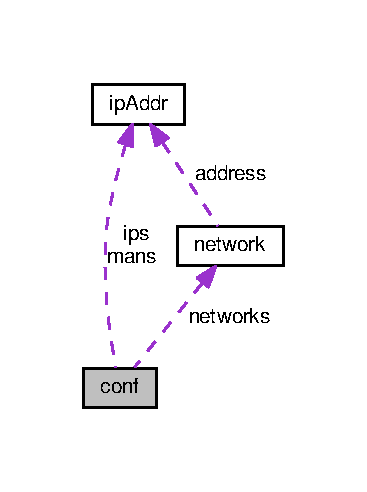
\includegraphics[width=176pt]{structconf__coll__graph}
\end{center}
\end{figure}
\subsection*{Campi}
\begin{DoxyCompactItemize}
\item 
int \hyperlink{structconf_aed28b971a9300be1236bcb25339ac4d0}{server\+\_\+port}\hypertarget{structconf_aed28b971a9300be1236bcb25339ac4d0}{}\label{structconf_aed28b971a9300be1236bcb25339ac4d0}

\begin{DoxyCompactList}\small\item\em Porta. \end{DoxyCompactList}\item 
int \hyperlink{structconf_ae224d1fc60f5ebff720813b981605090}{starting\+\_\+port}\hypertarget{structconf_ae224d1fc60f5ebff720813b981605090}{}\label{structconf_ae224d1fc60f5ebff720813b981605090}

\begin{DoxyCompactList}\small\item\em prima porta per i backup \end{DoxyCompactList}\item 
int \hyperlink{structconf_a0d988cd9a9e701b9f9c495f4ad7efabc}{port\+\_\+interval}\hypertarget{structconf_a0d988cd9a9e701b9f9c495f4ad7efabc}{}\label{structconf_a0d988cd9a9e701b9f9c495f4ad7efabc}

\begin{DoxyCompactList}\small\item\em intervallo di porte \end{DoxyCompactList}\item 
int \hyperlink{structconf_ac9533944c1cffeede9fa067bd962cde0}{To\+Zip}\hypertarget{structconf_ac9533944c1cffeede9fa067bd962cde0}{}\label{structconf_ac9533944c1cffeede9fa067bd962cde0}

\begin{DoxyCompactList}\small\item\em Se 0 non comprimerà i files, altrimenti sì \end{DoxyCompactList}\item 
uint64\+\_\+t \hyperlink{structconf_a66f027d14ec97608e7d4f902c0e1a2ef}{max\+Ram\+Amount}\hypertarget{structconf_a66f027d14ec97608e7d4f902c0e1a2ef}{}\label{structconf_a66f027d14ec97608e7d4f902c0e1a2ef}

\begin{DoxyCompactList}\small\item\em se un file sarà più piccolo della dimensione specificata verrà compresso \end{DoxyCompactList}\item 
int \hyperlink{structconf_af8e49667319b5c643337dfd47794245f}{allow\+Equals\+Deny\+\_\+nets}\hypertarget{structconf_af8e49667319b5c643337dfd47794245f}{}\label{structconf_af8e49667319b5c643337dfd47794245f}

\begin{DoxyCompactList}\small\item\em la lista di reti sarà blacklistata \end{DoxyCompactList}\item 
int \hyperlink{structconf_a29ff09d6dc81bcc5a4429b9729b88c05}{allow\+Equals\+Deny\+\_\+ips}\hypertarget{structconf_a29ff09d6dc81bcc5a4429b9729b88c05}{}\label{structconf_a29ff09d6dc81bcc5a4429b9729b88c05}

\begin{DoxyCompactList}\small\item\em la lista di host sarà blacklistata \end{DoxyCompactList}\item 
int \hyperlink{structconf_a4142b842e095d315af138c6aed12e76f}{nets\+No}\hypertarget{structconf_a4142b842e095d315af138c6aed12e76f}{}\label{structconf_a4142b842e095d315af138c6aed12e76f}

\begin{DoxyCompactList}\small\item\em Numero di reti in lista. \end{DoxyCompactList}\item 
\hyperlink{structnetwork}{network} $\ast$ \hyperlink{structconf_a6272ea163f134ef85d02fb0bf61b5a1e}{networks}\hypertarget{structconf_a6272ea163f134ef85d02fb0bf61b5a1e}{}\label{structconf_a6272ea163f134ef85d02fb0bf61b5a1e}

\begin{DoxyCompactList}\small\item\em referenza alla lista di reti \end{DoxyCompactList}\item 
int \hyperlink{structconf_adb85368e13aa7e3effcabb0949b9aa6e}{ips\+No}\hypertarget{structconf_adb85368e13aa7e3effcabb0949b9aa6e}{}\label{structconf_adb85368e13aa7e3effcabb0949b9aa6e}

\begin{DoxyCompactList}\small\item\em $<$ Numero di host in lista \end{DoxyCompactList}\item 
\hyperlink{unionipAddr}{ip\+Addr} $\ast$ \hyperlink{structconf_a9d55477addc26bcac7f17785c0b479b5}{ips}\hypertarget{structconf_a9d55477addc26bcac7f17785c0b479b5}{}\label{structconf_a9d55477addc26bcac7f17785c0b479b5}

\begin{DoxyCompactList}\small\item\em $<$ referenza alla lista di host \end{DoxyCompactList}\item 
int \hyperlink{structconf_aae47204ce4fb76b07907c991fd422666}{man\+No}\hypertarget{structconf_aae47204ce4fb76b07907c991fd422666}{}\label{structconf_aae47204ce4fb76b07907c991fd422666}

\begin{DoxyCompactList}\small\item\em Numero di host amministrativi in lista. \end{DoxyCompactList}\item 
\hyperlink{unionipAddr}{ip\+Addr} $\ast$ \hyperlink{structconf_a4e1650a523f01ccb65fda55aa2f2646d}{mans}\hypertarget{structconf_a4e1650a523f01ccb65fda55aa2f2646d}{}\label{structconf_a4e1650a523f01ccb65fda55aa2f2646d}

\begin{DoxyCompactList}\small\item\em referenza alla lista di amministratori \end{DoxyCompactList}\end{DoxyCompactItemize}


\subsection{Descrizione dettagliata}
Struttura contenete le configurazioni del server 

La documentazione per questa struct è stata generata a partire dal seguente file\+:\begin{DoxyCompactItemize}
\item 
Headers.\+h\end{DoxyCompactItemize}

\hypertarget{structconnection__t}{}\section{Riferimenti per la struct connection\+\_\+t}
\label{structconnection__t}\index{connection\+\_\+t@{connection\+\_\+t}}
\subsection*{Campi}
\begin{DoxyCompactItemize}
\item 
int {\bfseries socket}\hypertarget{structconnection__t_a8739936cfe1c4e9f23368e375c976c92}{}\label{structconnection__t_a8739936cfe1c4e9f23368e375c976c92}

\item 
struct sockaddr\+\_\+in {\bfseries client\+Data}\hypertarget{structconnection__t_a2b4d38d53b1ca15e78ff677f8e6fc761}{}\label{structconnection__t_a2b4d38d53b1ca15e78ff677f8e6fc761}

\item 
socklen\+\_\+t {\bfseries client\+Data\+Lenght}\hypertarget{structconnection__t_ada2a0ae1a1bcf2709cfda2d95e9ac1a1}{}\label{structconnection__t_ada2a0ae1a1bcf2709cfda2d95e9ac1a1}

\end{DoxyCompactItemize}


La documentazione per questa struct è stata generata a partire dal seguente file\+:\begin{DoxyCompactItemize}
\item 
Networking/Networking.\+h\end{DoxyCompactItemize}

\hypertarget{structfile__h}{}\section{Riferimenti per la struct file\+\_\+h}
\label{structfile__h}\index{file\+\_\+h@{file\+\_\+h}}


{\ttfamily \#include $<$Headers.\+h$>$}

\subsection*{Campi}
\begin{DoxyCompactItemize}
\item 
uint64\+\_\+t \hyperlink{structfile__h_aa060043d353f2e6ad89056b41d447db1}{dimension}\hypertarget{structfile__h_aa060043d353f2e6ad89056b41d447db1}{}\label{structfile__h_aa060043d353f2e6ad89056b41d447db1}

\begin{DoxyCompactList}\small\item\em dimensione del file non cifrato \end{DoxyCompactList}\item 
uint64\+\_\+t \hyperlink{structfile__h_ab38d74a27790a6f78dbdafa8abb22b53}{transfer\+\_\+dimension}\hypertarget{structfile__h_ab38d74a27790a6f78dbdafa8abb22b53}{}\label{structfile__h_ab38d74a27790a6f78dbdafa8abb22b53}

\begin{DoxyCompactList}\small\item\em dimensione trasmessa \end{DoxyCompactList}\item 
int \hyperlink{structfile__h_aa1bed54bf0f50c6cedab5592b87fe23c}{is\+Encoded}\hypertarget{structfile__h_aa1bed54bf0f50c6cedab5592b87fe23c}{}\label{structfile__h_aa1bed54bf0f50c6cedab5592b87fe23c}

\begin{DoxyCompactList}\small\item\em se 0 non codificato, altrimenti codificato \end{DoxyCompactList}\item 
time\+\_\+t \hyperlink{structfile__h_a2597abbe20de9abafd0b19f894bc4995}{time}\hypertarget{structfile__h_a2597abbe20de9abafd0b19f894bc4995}{}\label{structfile__h_a2597abbe20de9abafd0b19f894bc4995}

\begin{DoxyCompactList}\small\item\em data di trasmissione \end{DoxyCompactList}\item 
char \hyperlink{structfile__h_adb638eabdc439fe6ad101f8a482de3bd}{name} \mbox{[}55\mbox{]}\hypertarget{structfile__h_adb638eabdc439fe6ad101f8a482de3bd}{}\label{structfile__h_adb638eabdc439fe6ad101f8a482de3bd}

\begin{DoxyCompactList}\small\item\em nome originale del file \end{DoxyCompactList}\item 
char \hyperlink{structfile__h_aee04c560748989339f3a6fb430169428}{foo} \mbox{[}32\mbox{]}\hypertarget{structfile__h_aee04c560748989339f3a6fb430169428}{}\label{structfile__h_aee04c560748989339f3a6fb430169428}

\begin{DoxyCompactList}\small\item\em dati aggiuntivi \end{DoxyCompactList}\end{DoxyCompactItemize}


\subsection{Descrizione dettagliata}
Header del file di backup 

La documentazione per questa struct è stata generata a partire dal seguente file\+:\begin{DoxyCompactItemize}
\item 
Headers.\+h\end{DoxyCompactItemize}

\hypertarget{structidentify__answ__h}{}\section{Riferimenti per la struct identify\+\_\+answ\+\_\+h}
\label{structidentify__answ__h}\index{identify\+\_\+answ\+\_\+h@{identify\+\_\+answ\+\_\+h}}


{\ttfamily \#include $<$Headers.\+h$>$}

\subsection*{Campi}
\begin{DoxyCompactItemize}
\item 
char {\bfseries mw} \mbox{[}2\mbox{]}\hypertarget{structidentify__answ__h_afae2b93794a47b9581d77cc98e919314}{}\label{structidentify__answ__h_afae2b93794a47b9581d77cc98e919314}

\item 
int {\bfseries next\+Lenght}\hypertarget{structidentify__answ__h_ae7b384fb55a83e8013985d97c3d44a9a}{}\label{structidentify__answ__h_ae7b384fb55a83e8013985d97c3d44a9a}

\end{DoxyCompactItemize}


\subsection{Descrizione dettagliata}
Pacchetto di richiesta identificazione 

La documentazione per questa struct è stata generata a partire dal seguente file\+:\begin{DoxyCompactItemize}
\item 
Headers.\+h\end{DoxyCompactItemize}

\hypertarget{unionipAddr}{}\section{Riferimenti per la union ip\+Addr}
\label{unionipAddr}\index{ip\+Addr@{ip\+Addr}}
\subsection*{Campi}
\begin{DoxyCompactItemize}
\item 
uint8\+\_\+t {\bfseries parts} \mbox{[}4\mbox{]}\hypertarget{unionipAddr_a556df322f89f52547482d24855a13049}{}\label{unionipAddr_a556df322f89f52547482d24855a13049}

\item 
uint32\+\_\+t {\bfseries ip}\hypertarget{unionipAddr_a55faff16e5463af66104860af56d915e}{}\label{unionipAddr_a55faff16e5463af66104860af56d915e}

\end{DoxyCompactItemize}


La documentazione per questa union è stata generata a partire dal seguente file\+:\begin{DoxyCompactItemize}
\item 
comandi/Headers.\+h\end{DoxyCompactItemize}

\hypertarget{structmainpacket}{}\section{Riferimenti per la struct mainpacket}
\label{structmainpacket}\index{mainpacket@{mainpacket}}


{\ttfamily \#include $<$Headers.\+h$>$}

\subsection*{Campi}
\begin{DoxyCompactItemize}
\item 
char \hyperlink{structmainpacket_a9dffe3f8188b4a0b869d849c5d17f900}{mw} \mbox{[}2\mbox{]}\hypertarget{structmainpacket_a9dffe3f8188b4a0b869d849c5d17f900}{}\label{structmainpacket_a9dffe3f8188b4a0b869d849c5d17f900}

\begin{DoxyCompactList}\small\item\em Identificxatore del pacchetto. \end{DoxyCompactList}\item 
char \hyperlink{structmainpacket_addd5b2d5320ad3b172835f2cb1988eae}{data} \mbox{[}17\mbox{]}\hypertarget{structmainpacket_addd5b2d5320ad3b172835f2cb1988eae}{}\label{structmainpacket_addd5b2d5320ad3b172835f2cb1988eae}

\begin{DoxyCompactList}\small\item\em Dati presenti. \end{DoxyCompactList}\end{DoxyCompactItemize}


\subsection{Descrizione dettagliata}
La struttura Rappresenta un pacchetto generico ricevuto dal server U\+DP 

La documentazione per questa struct è stata generata a partire dal seguente file\+:\begin{DoxyCompactItemize}
\item 
Headers.\+h\end{DoxyCompactItemize}

\hypertarget{structnetwork}{}\section{Riferimenti per la struct network}
\label{structnetwork}\index{network@{network}}


{\ttfamily \#include $<$Headers.\+h$>$}



Diagramma di collaborazione per network\+:
% FIG 0
\subsection*{Campi}
\begin{DoxyCompactItemize}
\item 
\hyperlink{unionipAddr}{ip\+Addr} \hyperlink{structnetwork_aadfdf4cd8bd0c69641dbbdcc6376bb10}{address}\hypertarget{structnetwork_aadfdf4cd8bd0c69641dbbdcc6376bb10}{}\label{structnetwork_aadfdf4cd8bd0c69641dbbdcc6376bb10}

\begin{DoxyCompactList}\small\item\em ip \end{DoxyCompactList}\item 
unsigned int \hyperlink{structnetwork_a4b43d7f804814ac38a81108cfc538969}{net\+Mask}\hypertarget{structnetwork_a4b43d7f804814ac38a81108cfc538969}{}\label{structnetwork_a4b43d7f804814ac38a81108cfc538969}

\begin{DoxyCompactList}\small\item\em netmask \end{DoxyCompactList}\end{DoxyCompactItemize}


\subsection{Descrizione dettagliata}
Definizione di rete 

La documentazione per questa struct è stata generata a partire dal seguente file\+:\begin{DoxyCompactItemize}
\item 
comandi/Headers.\+h\end{DoxyCompactItemize}

\hypertarget{structpkey__identifier__t}{}\section{Riferimenti per la struct pkey\+\_\+identifier\+\_\+t}
\label{structpkey__identifier__t}\index{pkey\+\_\+identifier\+\_\+t@{pkey\+\_\+identifier\+\_\+t}}


{\ttfamily \#include $<$Headers.\+h$>$}

\subsection*{Campi}
\begin{DoxyCompactItemize}
\item 
int {\bfseries explen}\hypertarget{structpkey__identifier__t_a7729b33138069bdc3beb5dd03bea2613}{}\label{structpkey__identifier__t_a7729b33138069bdc3beb5dd03bea2613}

\item 
int {\bfseries nlen}\hypertarget{structpkey__identifier__t_a61cdeeb9e3bebcdcdaf1a8cbb8eaf186}{}\label{structpkey__identifier__t_a61cdeeb9e3bebcdcdaf1a8cbb8eaf186}

\end{DoxyCompactItemize}


\subsection{Descrizione dettagliata}
Pacchetto di richiesta chiave pubblica 

La documentazione per questa struct è stata generata a partire dal seguente file\+:\begin{DoxyCompactItemize}
\item 
Headers.\+h\end{DoxyCompactItemize}

\hypertarget{structsshconf}{}\section{Riferimenti per la struct sshconf}
\label{structsshconf}\index{sshconf@{sshconf}}


{\ttfamily \#include $<$Headers.\+h$>$}

\subsection*{Campi}
\begin{DoxyCompactItemize}
\item 
int \hyperlink{structsshconf_ac7a42459cfc0b74b311112a8213aea2f}{port}\hypertarget{structsshconf_ac7a42459cfc0b74b311112a8213aea2f}{}\label{structsshconf_ac7a42459cfc0b74b311112a8213aea2f}

\begin{DoxyCompactList}\small\item\em porta del terminale ssh \end{DoxyCompactList}\item 
char $\ast$ \hyperlink{structsshconf_a0f7971696b5f2cc4a30c31cfb2324083}{user}\hypertarget{structsshconf_a0f7971696b5f2cc4a30c31cfb2324083}{}\label{structsshconf_a0f7971696b5f2cc4a30c31cfb2324083}

\begin{DoxyCompactList}\small\item\em username \end{DoxyCompactList}\item 
char $\ast$ \hyperlink{structsshconf_a72e52ee8742a96bb28def3acb0996eef}{password}\hypertarget{structsshconf_a72e52ee8742a96bb28def3acb0996eef}{}\label{structsshconf_a72e52ee8742a96bb28def3acb0996eef}

\begin{DoxyCompactList}\small\item\em hash della password \end{DoxyCompactList}\item 
char $\ast$ \hyperlink{structsshconf_a4a8815987288dd2e91d0b52423bf4c08}{rsa}\hypertarget{structsshconf_a4a8815987288dd2e91d0b52423bf4c08}{}\label{structsshconf_a4a8815987288dd2e91d0b52423bf4c08}

\begin{DoxyCompactList}\small\item\em referenza al file con le chiavi rsa \end{DoxyCompactList}\item 
char $\ast$ \hyperlink{structsshconf_aaee9b07232c521cf70c3f4469b4180eb}{dsa}\hypertarget{structsshconf_aaee9b07232c521cf70c3f4469b4180eb}{}\label{structsshconf_aaee9b07232c521cf70c3f4469b4180eb}

\begin{DoxyCompactList}\small\item\em referenza al file con le chiavi dsa \end{DoxyCompactList}\item 
int \hyperlink{structsshconf_a63492312140e0a594d556bd187a601e0}{usepcap}\hypertarget{structsshconf_a63492312140e0a594d556bd187a601e0}{}\label{structsshconf_a63492312140e0a594d556bd187a601e0}

\begin{DoxyCompactList}\small\item\em se 0 non usare file pcap, altrimenti sì \end{DoxyCompactList}\item 
char $\ast$ \hyperlink{structsshconf_a43a1f28da9bffb5a86ccf7fad4e4d11d}{pcap}\hypertarget{structsshconf_a43a1f28da9bffb5a86ccf7fad4e4d11d}{}\label{structsshconf_a43a1f28da9bffb5a86ccf7fad4e4d11d}

\begin{DoxyCompactList}\small\item\em referenza al file pcap \end{DoxyCompactList}\end{DoxyCompactItemize}


\subsection{Descrizione dettagliata}
Configurazione S\+SH 

La documentazione per questa struct è stata generata a partire dal seguente file\+:\begin{DoxyCompactItemize}
\item 
Headers.\+h\end{DoxyCompactItemize}

\chapter{Documentazione dei file}
\hypertarget{aes_8c}{}\section{Riferimenti per il file A\+E\+S/aes.c}
\label{aes_8c}\index{A\+E\+S/aes.\+c@{A\+E\+S/aes.\+c}}


Cifratura A\+ES.  


{\ttfamily \#include $<$stdint.\+h$>$}\\*
{\ttfamily \#include $<$string.\+h$>$}\\*
{\ttfamily \#include \char`\"{}aes.\+h\char`\"{}}\\*
Grafo delle dipendenze di inclusione per aes.\+c\+:\nopagebreak
\begin{figure}[H]
\begin{center}
\leavevmode
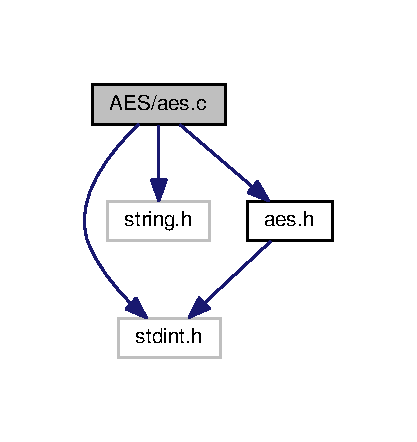
\includegraphics[width=200pt]{aes_8c__incl}
\end{center}
\end{figure}
\subsection*{Definizioni}
\begin{DoxyCompactItemize}
\item 
\#define {\bfseries Nb}~4\hypertarget{aes_8c_a1ae104196f1fc7af4751c5b9e07b1610}{}\label{aes_8c_a1ae104196f1fc7af4751c5b9e07b1610}

\item 
\#define {\bfseries B\+L\+O\+C\+K\+L\+EN}~16\hypertarget{aes_8c_ae1f92a72abcfa2a64173895807f3fa14}{}\label{aes_8c_ae1f92a72abcfa2a64173895807f3fa14}

\item 
\#define {\bfseries Nk}~8\hypertarget{aes_8c_a7b1938df390b1afe917e8baa663c22af}{}\label{aes_8c_a7b1938df390b1afe917e8baa663c22af}

\item 
\#define {\bfseries K\+E\+Y\+L\+EN}~32\hypertarget{aes_8c_ae6ae55940dfdf1155736df656d83a7cd}{}\label{aes_8c_ae6ae55940dfdf1155736df656d83a7cd}

\item 
\#define {\bfseries Nr}~14\hypertarget{aes_8c_a9d210afc812225ee0a0bcd51bb984246}{}\label{aes_8c_a9d210afc812225ee0a0bcd51bb984246}

\item 
\#define {\bfseries key\+Exp\+Size}~240\hypertarget{aes_8c_ac9922b8299100b46a11ece563fd23264}{}\label{aes_8c_ac9922b8299100b46a11ece563fd23264}

\item 
\#define {\bfseries M\+U\+L\+T\+I\+P\+L\+Y\+\_\+\+A\+S\+\_\+\+A\+\_\+\+F\+U\+N\+C\+T\+I\+ON}~0 /$\ast$$<$In alcuni casi utilizzare una chiamata a funzione invece di una definizione rende il codice più compatto ma lento. $\ast$/\hypertarget{aes_8c_a1dd86ce8e7ff32d6456f34c281c7e2a9}{}\label{aes_8c_a1dd86ce8e7ff32d6456f34c281c7e2a9}

\item 
\#define {\bfseries get\+S\+Box\+Value}(num)~sbox\mbox{[}num\mbox{]}\hypertarget{aes_8c_a5e1678341a98f95d48365ed9ccaa3586}{}\label{aes_8c_a5e1678341a98f95d48365ed9ccaa3586}

\item 
\#define {\bfseries get\+S\+Box\+Invert}(num)~rsbox\mbox{[}num\mbox{]}\hypertarget{aes_8c_a4223d41bc5587f9c0b6e499004403967}{}\label{aes_8c_a4223d41bc5587f9c0b6e499004403967}

\item 
\#define {\bfseries xtime}(x)~((x $<$$<$ 1) $^\wedge$ (((x $>$$>$ 7) \& 1) $\ast$ 0x1b))\hypertarget{aes_8c_ab6b4f6e4156553342ec4009bad2cc50e}{}\label{aes_8c_ab6b4f6e4156553342ec4009bad2cc50e}

\item 
\#define {\bfseries Multiply}(x,  y)
\end{DoxyCompactItemize}
\subsection*{Ridefinizioni di tipo (typedef)}
\begin{DoxyCompactItemize}
\item 
typedef uint8\+\_\+t {\bfseries state\+\_\+t}\mbox{[}4\mbox{]}\mbox{[}4\mbox{]}\hypertarget{aes_8c_a35dbb26673d196810a7f6eac0ac632ec}{}\label{aes_8c_a35dbb26673d196810a7f6eac0ac632ec}

\end{DoxyCompactItemize}
\subsection*{Funzioni}
\begin{DoxyCompactItemize}
\item 
void \hyperlink{aes_8c_a983d3da5e4e6f3d9ac0143787650ccb5}{Key\+Expansion} (void)\hypertarget{aes_8c_a983d3da5e4e6f3d9ac0143787650ccb5}{}\label{aes_8c_a983d3da5e4e6f3d9ac0143787650ccb5}

\begin{DoxyCompactList}\small\item\em Generazione delle chiavi intermedie. \end{DoxyCompactList}\item 
void \hyperlink{aes_8c_a153a141c4ff06edbb758b62c906bccb4}{Add\+Round\+Key} (uint8\+\_\+t round)
\begin{DoxyCompactList}\small\item\em Computazione della round\+Key nella matrice di stato. La chiave viene \char`\"{}\+Aggiunta\char`\"{} mediante X\+OR. \end{DoxyCompactList}\item 
void \hyperlink{aes_8c_a11159f2defb4de381f19ec1345995961}{Sub\+Bytes} (void)\hypertarget{aes_8c_a11159f2defb4de381f19ec1345995961}{}\label{aes_8c_a11159f2defb4de381f19ec1345995961}

\begin{DoxyCompactList}\small\item\em Compilazione dello stato mediante sbox. Viene sostituito il valore nella matrice di stato con il valore all\textquotesingle{}indice puntato dal valore contenuto in essa relativo al vettore S\+B\+OX. \end{DoxyCompactList}\item 
void \hyperlink{aes_8c_a45c39dd32ab250f98e34fcfdaae97af9}{Shift\+Rows} (void)\hypertarget{aes_8c_a45c39dd32ab250f98e34fcfdaae97af9}{}\label{aes_8c_a45c39dd32ab250f98e34fcfdaae97af9}

\begin{DoxyCompactList}\small\item\em Rotazione delle colonne della matrice. \end{DoxyCompactList}\item 
void \hyperlink{aes_8c_ad14c28ca3c74910fe263c68ba4cd49df}{Mix\+Columns} (void)\hypertarget{aes_8c_ad14c28ca3c74910fe263c68ba4cd49df}{}\label{aes_8c_ad14c28ca3c74910fe263c68ba4cd49df}

\begin{DoxyCompactList}\small\item\em Rotazione delle colonne. \end{DoxyCompactList}\item 
void \hyperlink{aes_8c_a448eb070583186878fb2d3ae5e68e081}{Inv\+Mix\+Columns} (void)\hypertarget{aes_8c_a448eb070583186878fb2d3ae5e68e081}{}\label{aes_8c_a448eb070583186878fb2d3ae5e68e081}

\begin{DoxyCompactList}\small\item\em Rotazione delle colonne inversa. \end{DoxyCompactList}\item 
void {\bfseries Inv\+Sub\+Bytes} (void)\hypertarget{aes_8c_a77cb391437e6b2484ae1713c38393033}{}\label{aes_8c_a77cb391437e6b2484ae1713c38393033}

\item 
void {\bfseries Inv\+Shift\+Rows} (void)\hypertarget{aes_8c_a0dbb125ca6b4eb68b3f0e0b19960a384}{}\label{aes_8c_a0dbb125ca6b4eb68b3f0e0b19960a384}

\item 
void \hyperlink{aes_8c_a068fd9934f544b4ce3b989b44434253d}{Cipher} (void)\hypertarget{aes_8c_a068fd9934f544b4ce3b989b44434253d}{}\label{aes_8c_a068fd9934f544b4ce3b989b44434253d}

\begin{DoxyCompactList}\small\item\em computazione del cifrario. \end{DoxyCompactList}\item 
void {\bfseries Inv\+Cipher} (void)\hypertarget{aes_8c_a45adbb908f044e7c6c0381d65ba1b6db}{}\label{aes_8c_a45adbb908f044e7c6c0381d65ba1b6db}

\item 
void \hyperlink{aes_8c_a5a93d43aab4c9f397697396ecd47f14c}{A\+E\+S\+\_\+\+E\+C\+B\+\_\+encrypt} (const uint8\+\_\+t $\ast$input, const uint8\+\_\+t $\ast$key, uint8\+\_\+t $\ast$output, const uint32\+\_\+t length)
\begin{DoxyCompactList}\small\item\em Cifratura La funcione cifrerà il testo in input con la chiave fornita. \end{DoxyCompactList}\item 
void \hyperlink{aes_8c_ae3175d2f455bd50271c88f1458bf7df9}{A\+E\+S\+\_\+\+E\+C\+B\+\_\+decrypt} (const uint8\+\_\+t $\ast$input, const uint8\+\_\+t $\ast$key, uint8\+\_\+t $\ast$output, const uint32\+\_\+t length)
\begin{DoxyCompactList}\small\item\em Decifratura La funcione decifrerà il testo in input con la chiave fornita. \end{DoxyCompactList}\end{DoxyCompactItemize}
\subsection*{Variabili}
\begin{DoxyCompactItemize}
\item 
state\+\_\+t $\ast$ {\bfseries state}\hypertarget{aes_8c_ad180be797ec209ed2712c000b4fd536f}{}\label{aes_8c_ad180be797ec209ed2712c000b4fd536f}

\item 
uint8\+\_\+t {\bfseries Round\+Key} \mbox{[}key\+Exp\+Size\mbox{]}\hypertarget{aes_8c_ad550b81bd148e6cfa25f5b185089beec}{}\label{aes_8c_ad550b81bd148e6cfa25f5b185089beec}

\item 
const uint8\+\_\+t $\ast$ {\bfseries Key}\hypertarget{aes_8c_a0a8f142857a68487ebfeb023024d4e85}{}\label{aes_8c_a0a8f142857a68487ebfeb023024d4e85}

\item 
const uint8\+\_\+t {\bfseries sbox} \mbox{[}256\mbox{]}
\item 
const uint8\+\_\+t {\bfseries rsbox} \mbox{[}256\mbox{]}
\item 
const uint8\+\_\+t {\bfseries Rcon} \mbox{[}$\,$\mbox{]}
\end{DoxyCompactItemize}


\subsection{Descrizione dettagliata}
Cifratura A\+ES. 

\begin{DoxyVersion}{Versione}
1.\+0 
\end{DoxyVersion}
\begin{DoxyAuthor}{Autore}
Stefano 
\end{DoxyAuthor}
\begin{DoxyDate}{Data}
06-\/11-\/2017 
\end{DoxyDate}


\subsection{Documentazione delle definizioni}
\index{aes.\+c@{aes.\+c}!Multiply@{Multiply}}
\index{Multiply@{Multiply}!aes.\+c@{aes.\+c}}
\subsubsection[{\texorpdfstring{Multiply}{Multiply}}]{\setlength{\rightskip}{0pt plus 5cm}\#define Multiply(
\begin{DoxyParamCaption}
\item[{}]{x, }
\item[{}]{y}
\end{DoxyParamCaption}
)}\hypertarget{aes_8c_aca7cce176b8cdd27f61d3dcf5910b6bd}{}\label{aes_8c_aca7cce176b8cdd27f61d3dcf5910b6bd}
{\bfseries Valore\+:}
\begin{DoxyCode}
(  ((y & 1) * x) ^                              \(\backslash\)
      ((y>>1 & 1) * xtime(x)) ^                       \(\backslash\)
      ((y>>2 & 1) * xtime(xtime(x))) ^                \(\backslash\)
      ((y>>3 & 1) * xtime(xtime(xtime(x)))) ^         \(\backslash\)
        ((y>>4 & 1) * xtime(xtime(xtime(xtime(x)))))) \(\backslash\)
\end{DoxyCode}


\subsection{Documentazione delle funzioni}
\index{aes.\+c@{aes.\+c}!Add\+Round\+Key@{Add\+Round\+Key}}
\index{Add\+Round\+Key@{Add\+Round\+Key}!aes.\+c@{aes.\+c}}
\subsubsection[{\texorpdfstring{Add\+Round\+Key(uint8\+\_\+t round)}{AddRoundKey(uint8_t round)}}]{\setlength{\rightskip}{0pt plus 5cm}void Add\+Round\+Key (
\begin{DoxyParamCaption}
\item[{uint8\+\_\+t}]{round}
\end{DoxyParamCaption}
)}\hypertarget{aes_8c_a153a141c4ff06edbb758b62c906bccb4}{}\label{aes_8c_a153a141c4ff06edbb758b62c906bccb4}


Computazione della round\+Key nella matrice di stato. La chiave viene \char`\"{}\+Aggiunta\char`\"{} mediante X\+OR. 


\begin{DoxyParams}[1]{Parametri}
\mbox{\tt in}  & {\em round} & Round\+Key in input \\
\hline
\end{DoxyParams}
\index{aes.\+c@{aes.\+c}!A\+E\+S\+\_\+\+E\+C\+B\+\_\+decrypt@{A\+E\+S\+\_\+\+E\+C\+B\+\_\+decrypt}}
\index{A\+E\+S\+\_\+\+E\+C\+B\+\_\+decrypt@{A\+E\+S\+\_\+\+E\+C\+B\+\_\+decrypt}!aes.\+c@{aes.\+c}}
\subsubsection[{\texorpdfstring{A\+E\+S\+\_\+\+E\+C\+B\+\_\+decrypt(const uint8\+\_\+t $\ast$input, const uint8\+\_\+t $\ast$key, uint8\+\_\+t $\ast$output, const uint32\+\_\+t length)}{AES_ECB_decrypt(const uint8_t *input, const uint8_t *key, uint8_t *output, const uint32_t length)}}]{\setlength{\rightskip}{0pt plus 5cm}void A\+E\+S\+\_\+\+E\+C\+B\+\_\+decrypt (
\begin{DoxyParamCaption}
\item[{const uint8\+\_\+t $\ast$}]{input, }
\item[{const uint8\+\_\+t $\ast$}]{key, }
\item[{uint8\+\_\+t $\ast$}]{output, }
\item[{const uint32\+\_\+t}]{length}
\end{DoxyParamCaption}
)}\hypertarget{aes_8c_ae3175d2f455bd50271c88f1458bf7df9}{}\label{aes_8c_ae3175d2f455bd50271c88f1458bf7df9}


Decifratura La funcione decifrerà il testo in input con la chiave fornita. 


\begin{DoxyParams}{Parametri}
{\em input\mbox{[}in\mbox{]}} & Testo cifrato in input \\
\hline
{\em key\mbox{[}in\mbox{]}} & Chiave di cifratura a 256 bit \\
\hline
{\em output\mbox{[}out\mbox{]}} & Testo decifrato in output \\
\hline
{\em length\mbox{[}in\mbox{]}} & Lunghezza del testo in input \\
\hline
\end{DoxyParams}
\index{aes.\+c@{aes.\+c}!A\+E\+S\+\_\+\+E\+C\+B\+\_\+encrypt@{A\+E\+S\+\_\+\+E\+C\+B\+\_\+encrypt}}
\index{A\+E\+S\+\_\+\+E\+C\+B\+\_\+encrypt@{A\+E\+S\+\_\+\+E\+C\+B\+\_\+encrypt}!aes.\+c@{aes.\+c}}
\subsubsection[{\texorpdfstring{A\+E\+S\+\_\+\+E\+C\+B\+\_\+encrypt(const uint8\+\_\+t $\ast$input, const uint8\+\_\+t $\ast$key, uint8\+\_\+t $\ast$output, const uint32\+\_\+t length)}{AES_ECB_encrypt(const uint8_t *input, const uint8_t *key, uint8_t *output, const uint32_t length)}}]{\setlength{\rightskip}{0pt plus 5cm}void A\+E\+S\+\_\+\+E\+C\+B\+\_\+encrypt (
\begin{DoxyParamCaption}
\item[{const uint8\+\_\+t $\ast$}]{input, }
\item[{const uint8\+\_\+t $\ast$}]{key, }
\item[{uint8\+\_\+t $\ast$}]{output, }
\item[{const uint32\+\_\+t}]{length}
\end{DoxyParamCaption}
)}\hypertarget{aes_8c_a5a93d43aab4c9f397697396ecd47f14c}{}\label{aes_8c_a5a93d43aab4c9f397697396ecd47f14c}


Cifratura La funcione cifrerà il testo in input con la chiave fornita. 


\begin{DoxyParams}{Parametri}
{\em input\mbox{[}in\mbox{]}} & Testo in chiaro in input \\
\hline
{\em key\mbox{[}in\mbox{]}} & Chiave di cifratura a 256 bit \\
\hline
{\em output\mbox{[}out\mbox{]}} & Testo cifrato in output \\
\hline
{\em length\mbox{[}in\mbox{]}} & Lunghezza del testo in chiaro \\
\hline
\end{DoxyParams}


\subsection{Documentazione delle variabili}
\index{aes.\+c@{aes.\+c}!Rcon@{Rcon}}
\index{Rcon@{Rcon}!aes.\+c@{aes.\+c}}
\subsubsection[{\texorpdfstring{Rcon}{Rcon}}]{\setlength{\rightskip}{0pt plus 5cm}const uint8\+\_\+t Rcon\mbox{[}$\,$\mbox{]}}\hypertarget{aes_8c_a25c64607a5017b10739ee8c6547f6996}{}\label{aes_8c_a25c64607a5017b10739ee8c6547f6996}
{\bfseries Valore iniziale\+:}
\begin{DoxyCode}
= \{
        0x8d, 0x01, 0x02, 0x04, 0x08,
        0x10, 0x20, 0x40, 0x80, 0x1b,
        0x36, 0x6c, 0xd8, 0xab, 0x4d\}
\end{DoxyCode}
\index{aes.\+c@{aes.\+c}!rsbox@{rsbox}}
\index{rsbox@{rsbox}!aes.\+c@{aes.\+c}}
\subsubsection[{\texorpdfstring{rsbox}{rsbox}}]{\setlength{\rightskip}{0pt plus 5cm}const uint8\+\_\+t rsbox\mbox{[}256\mbox{]}}\hypertarget{aes_8c_a5fb4523234538d83676ef33a45b18fd1}{}\label{aes_8c_a5fb4523234538d83676ef33a45b18fd1}
{\bfseries Valore iniziale\+:}
\begin{DoxyCode}
= \{
        0x52, 0x09, 0x6a, 0xd5, 0x30, 0x36, 0xa5, 0x38, 0xbf, 0x40, 0xa3, 0x9e, 0x81, 0xf3, 0xd7, 0xfb,
        0x7c, 0xe3, 0x39, 0x82, 0x9b, 0x2f, 0xff, 0x87, 0x34, 0x8e, 0x43, 0x44, 0xc4, 0xde, 0xe9, 0xcb,
        0x54, 0x7b, 0x94, 0x32, 0xa6, 0xc2, 0x23, 0x3d, 0xee, 0x4c, 0x95, 0x0b, 0x42, 0xfa, 0xc3, 0x4e,
        0x08, 0x2e, 0xa1, 0x66, 0x28, 0xd9, 0x24, 0xb2, 0x76, 0x5b, 0xa2, 0x49, 0x6d, 0x8b, 0xd1, 0x25,
        0x72, 0xf8, 0xf6, 0x64, 0x86, 0x68, 0x98, 0x16, 0xd4, 0xa4, 0x5c, 0xcc, 0x5d, 0x65, 0xb6, 0x92,
        0x6c, 0x70, 0x48, 0x50, 0xfd, 0xed, 0xb9, 0xda, 0x5e, 0x15, 0x46, 0x57, 0xa7, 0x8d, 0x9d, 0x84,
        0x90, 0xd8, 0xab, 0x00, 0x8c, 0xbc, 0xd3, 0x0a, 0xf7, 0xe4, 0x58, 0x05, 0xb8, 0xb3, 0x45, 0x06,
        0xd0, 0x2c, 0x1e, 0x8f, 0xca, 0x3f, 0x0f, 0x02, 0xc1, 0xaf, 0xbd, 0x03, 0x01, 0x13, 0x8a, 0x6b,
        0x3a, 0x91, 0x11, 0x41, 0x4f, 0x67, 0xdc, 0xea, 0x97, 0xf2, 0xcf, 0xce, 0xf0, 0xb4, 0xe6, 0x73,
        0x96, 0xac, 0x74, 0x22, 0xe7, 0xad, 0x35, 0x85, 0xe2, 0xf9, 0x37, 0xe8, 0x1c, 0x75, 0xdf, 0x6e,
        0x47, 0xf1, 0x1a, 0x71, 0x1d, 0x29, 0xc5, 0x89, 0x6f, 0xb7, 0x62, 0x0e, 0xaa, 0x18, 0xbe, 0x1b,
        0xfc, 0x56, 0x3e, 0x4b, 0xc6, 0xd2, 0x79, 0x20, 0x9a, 0xdb, 0xc0, 0xfe, 0x78, 0xcd, 0x5a, 0xf4,
        0x1f, 0xdd, 0xa8, 0x33, 0x88, 0x07, 0xc7, 0x31, 0xb1, 0x12, 0x10, 0x59, 0x27, 0x80, 0xec, 0x5f,
        0x60, 0x51, 0x7f, 0xa9, 0x19, 0xb5, 0x4a, 0x0d, 0x2d, 0xe5, 0x7a, 0x9f, 0x93, 0xc9, 0x9c, 0xef,
        0xa0, 0xe0, 0x3b, 0x4d, 0xae, 0x2a, 0xf5, 0xb0, 0xc8, 0xeb, 0xbb, 0x3c, 0x83, 0x53, 0x99, 0x61,
        0x17, 0x2b, 0x04, 0x7e, 0xba, 0x77, 0xd6, 0x26, 0xe1, 0x69, 0x14, 0x63, 0x55, 0x21, 0x0c, 0x7d\}
\end{DoxyCode}
\index{aes.\+c@{aes.\+c}!sbox@{sbox}}
\index{sbox@{sbox}!aes.\+c@{aes.\+c}}
\subsubsection[{\texorpdfstring{sbox}{sbox}}]{\setlength{\rightskip}{0pt plus 5cm}const uint8\+\_\+t sbox\mbox{[}256\mbox{]}}\hypertarget{aes_8c_adc15aeb43c81de1162045eedf437f407}{}\label{aes_8c_adc15aeb43c81de1162045eedf437f407}
{\bfseries Valore iniziale\+:}
\begin{DoxyCode}
= \{
        
        0x63, 0x7c, 0x77, 0x7b, 0xf2, 0x6b, 0x6f, 0xc5, 0x30, 0x01, 0x67, 0x2b, 0xfe, 0xd7, 0xab, 0x76,
        0xca, 0x82, 0xc9, 0x7d, 0xfa, 0x59, 0x47, 0xf0, 0xad, 0xd4, 0xa2, 0xaf, 0x9c, 0xa4, 0x72, 0xc0,
        0xb7, 0xfd, 0x93, 0x26, 0x36, 0x3f, 0xf7, 0xcc, 0x34, 0xa5, 0xe5, 0xf1, 0x71, 0xd8, 0x31, 0x15,
        0x04, 0xc7, 0x23, 0xc3, 0x18, 0x96, 0x05, 0x9a, 0x07, 0x12, 0x80, 0xe2, 0xeb, 0x27, 0xb2, 0x75,
        0x09, 0x83, 0x2c, 0x1a, 0x1b, 0x6e, 0x5a, 0xa0, 0x52, 0x3b, 0xd6, 0xb3, 0x29, 0xe3, 0x2f, 0x84,
        0x53, 0xd1, 0x00, 0xed, 0x20, 0xfc, 0xb1, 0x5b, 0x6a, 0xcb, 0xbe, 0x39, 0x4a, 0x4c, 0x58, 0xcf,
        0xd0, 0xef, 0xaa, 0xfb, 0x43, 0x4d, 0x33, 0x85, 0x45, 0xf9, 0x02, 0x7f, 0x50, 0x3c, 0x9f, 0xa8,
        0x51, 0xa3, 0x40, 0x8f, 0x92, 0x9d, 0x38, 0xf5, 0xbc, 0xb6, 0xda, 0x21, 0x10, 0xff, 0xf3, 0xd2,
        0xcd, 0x0c, 0x13, 0xec, 0x5f, 0x97, 0x44, 0x17, 0xc4, 0xa7, 0x7e, 0x3d, 0x64, 0x5d, 0x19, 0x73,
        0x60, 0x81, 0x4f, 0xdc, 0x22, 0x2a, 0x90, 0x88, 0x46, 0xee, 0xb8, 0x14, 0xde, 0x5e, 0x0b, 0xdb,
        0xe0, 0x32, 0x3a, 0x0a, 0x49, 0x06, 0x24, 0x5c, 0xc2, 0xd3, 0xac, 0x62, 0x91, 0x95, 0xe4, 0x79,
        0xe7, 0xc8, 0x37, 0x6d, 0x8d, 0xd5, 0x4e, 0xa9, 0x6c, 0x56, 0xf4, 0xea, 0x65, 0x7a, 0xae, 0x08,
        0xba, 0x78, 0x25, 0x2e, 0x1c, 0xa6, 0xb4, 0xc6, 0xe8, 0xdd, 0x74, 0x1f, 0x4b, 0xbd, 0x8b, 0x8a,
        0x70, 0x3e, 0xb5, 0x66, 0x48, 0x03, 0xf6, 0x0e, 0x61, 0x35, 0x57, 0xb9, 0x86, 0xc1, 0x1d, 0x9e,
        0xe1, 0xf8, 0x98, 0x11, 0x69, 0xd9, 0x8e, 0x94, 0x9b, 0x1e, 0x87, 0xe9, 0xce, 0x55, 0x28, 0xdf,
        0x8c, 0xa1, 0x89, 0x0d, 0xbf, 0xe6, 0x42, 0x68, 0x41, 0x99, 0x2d, 0x0f, 0xb0, 0x54, 0xbb, 0x16\}
\end{DoxyCode}

\hypertarget{base32_8c}{}\section{Riferimenti per il file B\+A\+S\+E\+\_\+encoding/base32.c}
\label{base32_8c}\index{B\+A\+S\+E\+\_\+encoding/base32.\+c@{B\+A\+S\+E\+\_\+encoding/base32.\+c}}


Codifica base32.  


{\ttfamily \#include $<$assert.\+h$>$}\\*
{\ttfamily \#include $<$limits.\+h$>$}\\*
{\ttfamily \#include \char`\"{}base32.\+h\char`\"{}}\\*
Grafo delle dipendenze di inclusione per base32.\+c\+:
% FIG 0
\subsection*{Definizioni}
\begin{DoxyCompactItemize}
\item 
\#define {\bfseries min}(x,  y)~(x $<$ y ? x \+: y)\hypertarget{base32_8c_abb702d8b501669a23aa0ab3b281b9384}{}\label{base32_8c_abb702d8b501669a23aa0ab3b281b9384}

\end{DoxyCompactItemize}
\subsection*{Funzioni}
\begin{DoxyCompactItemize}
\item 
size\+\_\+t \hyperlink{base32_8c_ae5a4361671bd789618699659b98aefcb_ae5a4361671bd789618699659b98aefcb}{base32\+\_\+decode} (const unsigned char $\ast$coded, unsigned char $\ast$plain)
\begin{DoxyCompactList}\small\item\em Decodifica in base32 La funzione decodifica la stringa in input in base32. \end{DoxyCompactList}\item 
void \hyperlink{base32_8c_a17ec37ce739803d9b75109d5e00a3d40_a17ec37ce739803d9b75109d5e00a3d40}{base32\+\_\+encode} (const unsigned char $\ast$plain, size\+\_\+t len, unsigned char $\ast$coded)
\begin{DoxyCompactList}\small\item\em Codifica in base32 La funzione codifica la stringa in input in base32. \end{DoxyCompactList}\end{DoxyCompactItemize}


\subsection{Descrizione dettagliata}
Codifica base32. 

\begin{DoxyVersion}{Versione}
1.\+0 
\end{DoxyVersion}
\begin{DoxyAuthor}{Autore}
Stefano 
\end{DoxyAuthor}
\begin{DoxyDate}{Data}
10-\/11-\/2017 
\end{DoxyDate}


\subsection{Documentazione delle funzioni}
\index{base32.\+c@{base32.\+c}!base32\+\_\+decode@{base32\+\_\+decode}}
\index{base32\+\_\+decode@{base32\+\_\+decode}!base32.\+c@{base32.\+c}}
\subsubsection[{\texorpdfstring{base32\+\_\+decode(const unsigned char $\ast$coded, unsigned char $\ast$plain)}{base32_decode(const unsigned char *coded, unsigned char *plain)}}]{\setlength{\rightskip}{0pt plus 5cm}size\+\_\+t base32\+\_\+decode (
\begin{DoxyParamCaption}
\item[{const unsigned char $\ast$}]{coded, }
\item[{unsigned char $\ast$}]{plain}
\end{DoxyParamCaption}
)}\hypertarget{base32_8c_ae5a4361671bd789618699659b98aefcb_ae5a4361671bd789618699659b98aefcb}{}\label{base32_8c_ae5a4361671bd789618699659b98aefcb_ae5a4361671bd789618699659b98aefcb}


Decodifica in base32 La funzione decodifica la stringa in input in base32. 


\begin{DoxyParams}{Parametri}
{\em coded\mbox{[}in\mbox{]}} & La sequenza codificata \\
\hline
{\em plain\mbox{[}out\mbox{]}} & La sequaneza decodificata \\
\hline
\end{DoxyParams}
\begin{DoxyReturn}{Restituisce}
Numero dei caratteri scritti 
\end{DoxyReturn}
\index{base32.\+c@{base32.\+c}!base32\+\_\+encode@{base32\+\_\+encode}}
\index{base32\+\_\+encode@{base32\+\_\+encode}!base32.\+c@{base32.\+c}}
\subsubsection[{\texorpdfstring{base32\+\_\+encode(const unsigned char $\ast$plain, size\+\_\+t len, unsigned char $\ast$coded)}{base32_encode(const unsigned char *plain, size_t len, unsigned char *coded)}}]{\setlength{\rightskip}{0pt plus 5cm}void base32\+\_\+encode (
\begin{DoxyParamCaption}
\item[{const unsigned char $\ast$}]{plain, }
\item[{size\+\_\+t}]{len, }
\item[{unsigned char $\ast$}]{coded}
\end{DoxyParamCaption}
)}\hypertarget{base32_8c_a17ec37ce739803d9b75109d5e00a3d40_a17ec37ce739803d9b75109d5e00a3d40}{}\label{base32_8c_a17ec37ce739803d9b75109d5e00a3d40_a17ec37ce739803d9b75109d5e00a3d40}


Codifica in base32 La funzione codifica la stringa in input in base32. 


\begin{DoxyParams}{Parametri}
{\em coded\mbox{[}in\mbox{]}} & La sequenza da codificare \\
\hline
{\em plain\mbox{[}out\mbox{]}} & La sequaneza codificata \\
\hline
\end{DoxyParams}

\hypertarget{client_8cpp}{}\section{Riferimenti per il file client.\+cpp}
\label{client_8cpp}\index{client.\+cpp@{client.\+cpp}}


Client.  


{\ttfamily \#include $<$cstdio$>$}\\*
{\ttfamily \#include $<$cstdlib$>$}\\*
{\ttfamily \#include $<$ctime$>$}\\*
{\ttfamily \#include $<$cinttypes$>$}\\*
{\ttfamily \#include $<$csignal$>$}\\*
{\ttfamily \#include \char`\"{}Networking/\+Networking.\+h\char`\"{}}\\*
{\ttfamily \#include \char`\"{}B\+A\+S\+E\+\_\+encoding/base32.\+h\char`\"{}}\\*
{\ttfamily \#include \char`\"{}File\+System/\+F\+S.\+h\char`\"{}}\\*
{\ttfamily \#include \char`\"{}Headers.\+h\char`\"{}}\\*
{\ttfamily \#include \char`\"{}A\+E\+S/aes.\+h\char`\"{}}\\*
{\ttfamily \#include \char`\"{}config/config.\+h\char`\"{}}\\*
Grafo delle dipendenze di inclusione per client.\+cpp\+:\nopagebreak
\begin{figure}[H]
\begin{center}
\leavevmode
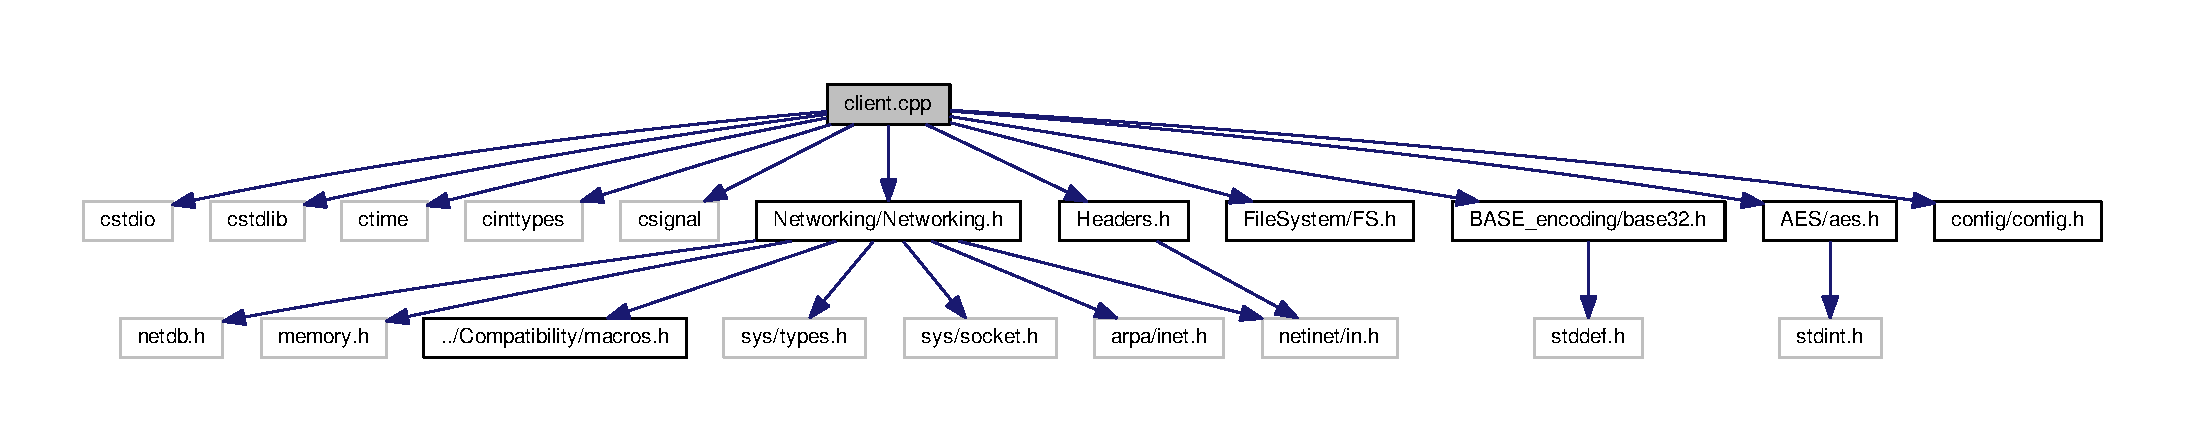
\includegraphics[width=350pt]{client_8cpp__incl}
\end{center}
\end{figure}
\subsection*{Definizioni}
\begin{DoxyCompactItemize}
\item 
\#define {\bfseries \+\_\+\+F\+I\+L\+E\+\_\+\+O\+F\+F\+S\+E\+T\+\_\+\+B\+I\+TS}~64\hypertarget{client_8cpp_a44d01ba0a136b8e27ad362f5a823d14e}{}\label{client_8cpp_a44d01ba0a136b8e27ad362f5a823d14e}

\end{DoxyCompactItemize}
\subsection*{Funzioni}
\begin{DoxyCompactItemize}
\item 
int \hyperlink{client_8cpp_a56e13ca67f5209b06bb1f1776550519e}{load\+Cfg} (char $\ast$config\+File)
\begin{DoxyCompactList}\small\item\em Caricamento della configurazione da file. \end{DoxyCompactList}\item 
int \hyperlink{client_8cpp_abd98a7bbb79f610827af69e06b435bbd}{ask\+Identity} (\hyperlink{structconnection__t}{connection\+\_\+t} socket)
\begin{DoxyCompactList}\small\item\em Richiesta di identità del server Viene richiesta al server la firma digitale di una stringa casuale generata dal client, quindi viene verificata mediante la chiave memorizzata in memoria. \end{DoxyCompactList}\item 
void \hyperlink{client_8cpp_a720f3388952905f8678f7311e921d1e7}{save\+Pkey} (\hyperlink{structconnection__t}{connection\+\_\+t} server)
\begin{DoxyCompactList}\small\item\em Salva una chiave pubblica in memoria La funzione richiederà al server la sua chiave pubblica e la memorizzerà in un file .public in memoria. \end{DoxyCompactList}\item 
int \hyperlink{client_8cpp_a4b5c13bd3f6431ce2b14d8bd5137a78a}{new\+Bak} (int port)
\begin{DoxyCompactList}\small\item\em La funzione inizia la trasmissione di un nuovo backup. \end{DoxyCompactList}\item 
int {\bfseries main} (int argc, char $\ast$$\ast$argv)\hypertarget{client_8cpp_a3c04138a5bfe5d72780bb7e82a18e627}{}\label{client_8cpp_a3c04138a5bfe5d72780bb7e82a18e627}

\end{DoxyCompactItemize}
\subsection*{Variabili}
\begin{DoxyCompactItemize}
\item 
int {\bfseries server\+\_\+port}\hypertarget{client_8cpp_af204d2d7af5cc273a2b38359c4c09c99}{}\label{client_8cpp_af204d2d7af5cc273a2b38359c4c09c99}

\item 
char $\ast$ {\bfseries server\+\_\+ip}\hypertarget{client_8cpp_a182d69acd4e02e6c0a027622a4556e53}{}\label{client_8cpp_a182d69acd4e02e6c0a027622a4556e53}

\item 
int {\bfseries is\+Encrypted}\hypertarget{client_8cpp_a1f2adafcac1b6ab58e9d3e9a9d219032}{}\label{client_8cpp_a1f2adafcac1b6ab58e9d3e9a9d219032}

\item 
int {\bfseries timeout}\hypertarget{client_8cpp_a493b57f443cc38b3d3df9c1e584d9d82}{}\label{client_8cpp_a493b57f443cc38b3d3df9c1e584d9d82}

\item 
char $\ast$$\ast$ {\bfseries files}\hypertarget{client_8cpp_a047d85a0e14d2ae13523bab2ed49f70b}{}\label{client_8cpp_a047d85a0e14d2ae13523bab2ed49f70b}

\item 
int {\bfseries file\+Numbers} = 0\hypertarget{client_8cpp_abdb4ba2d19a986e198505a1f263a1acd}{}\label{client_8cpp_abdb4ba2d19a986e198505a1f263a1acd}

\item 
int {\bfseries transfer\+\_\+block\+\_\+size}\hypertarget{client_8cpp_ad7e838552138781c9e6bc1606c2b1660}{}\label{client_8cpp_ad7e838552138781c9e6bc1606c2b1660}

\item 
char {\bfseries key} \mbox{[}32\mbox{]}\hypertarget{client_8cpp_aba8ec8b73c06b7c981b67e88184a1d08}{}\label{client_8cpp_aba8ec8b73c06b7c981b67e88184a1d08}

\item 
int {\bfseries interval}\hypertarget{client_8cpp_ae0c690118932b32ef40a74bb6a259acd}{}\label{client_8cpp_ae0c690118932b32ef40a74bb6a259acd}

\item 
uint8\+\_\+t $\ast$ {\bfseries data}\hypertarget{client_8cpp_abe222f6d3581e7920dcad5306cc906a8}{}\label{client_8cpp_abe222f6d3581e7920dcad5306cc906a8}

\item 
char $\ast$$\ast$ {\bfseries file}\hypertarget{client_8cpp_ab8055e05865bc04373bc4e75fedf2d19}{}\label{client_8cpp_ab8055e05865bc04373bc4e75fedf2d19}

\item 
char {\bfseries configF} \mbox{[}512\mbox{]}\hypertarget{client_8cpp_a24ef95dbb465c74790c9a6e9de1e17c0}{}\label{client_8cpp_a24ef95dbb465c74790c9a6e9de1e17c0}

\end{DoxyCompactItemize}


\subsection{Descrizione dettagliata}
Client. 

\begin{DoxyVersion}{Versione}
1.\+0 
\end{DoxyVersion}
\begin{DoxyAuthor}{Autore}
Stefano 
\end{DoxyAuthor}
\begin{DoxyDate}{Data}
28-\/10-\/2017 
\end{DoxyDate}


\subsection{Documentazione delle funzioni}
\index{client.\+cpp@{client.\+cpp}!ask\+Identity@{ask\+Identity}}
\index{ask\+Identity@{ask\+Identity}!client.\+cpp@{client.\+cpp}}
\subsubsection[{\texorpdfstring{ask\+Identity(connection\+\_\+t socket)}{askIdentity(connection_t socket)}}]{\setlength{\rightskip}{0pt plus 5cm}int ask\+Identity (
\begin{DoxyParamCaption}
\item[{{\bf connection\+\_\+t}}]{socket}
\end{DoxyParamCaption}
)}\hypertarget{client_8cpp_abd98a7bbb79f610827af69e06b435bbd}{}\label{client_8cpp_abd98a7bbb79f610827af69e06b435bbd}


Richiesta di identità del server Viene richiesta al server la firma digitale di una stringa casuale generata dal client, quindi viene verificata mediante la chiave memorizzata in memoria. 


\begin{DoxyParams}{Parametri}
{\em socket\mbox{[}in\mbox{]}} & struttura parametri di connessione \\
\hline
\end{DoxyParams}
\begin{DoxyReturn}{Restituisce}
-\/10 in caso il file relativo al server non esista o non sia accessibile, 1 in caso di verifica esatta, 0 altriemeti 
\end{DoxyReturn}
\index{client.\+cpp@{client.\+cpp}!load\+Cfg@{load\+Cfg}}
\index{load\+Cfg@{load\+Cfg}!client.\+cpp@{client.\+cpp}}
\subsubsection[{\texorpdfstring{load\+Cfg(char $\ast$config\+File)}{loadCfg(char *configFile)}}]{\setlength{\rightskip}{0pt plus 5cm}int load\+Cfg (
\begin{DoxyParamCaption}
\item[{char $\ast$}]{config\+File}
\end{DoxyParamCaption}
)}\hypertarget{client_8cpp_a56e13ca67f5209b06bb1f1776550519e}{}\label{client_8cpp_a56e13ca67f5209b06bb1f1776550519e}


Caricamento della configurazione da file. 


\begin{DoxyParams}{Parametri}
{\em config\+File\mbox{[}in\mbox{]}} & Nome del file di configurazione \\
\hline
\end{DoxyParams}
\begin{DoxyReturn}{Restituisce}
0 in caso di riuscita, -\/1 altrimenti 
\end{DoxyReturn}
\begin{DoxyRefDesc}{Bug}
\item[\hyperlink{bug__bug000001}{Bug}]In caso una proprietà non sia presente segfault \end{DoxyRefDesc}
\index{client.\+cpp@{client.\+cpp}!new\+Bak@{new\+Bak}}
\index{new\+Bak@{new\+Bak}!client.\+cpp@{client.\+cpp}}
\subsubsection[{\texorpdfstring{new\+Bak(int port)}{newBak(int port)}}]{\setlength{\rightskip}{0pt plus 5cm}int new\+Bak (
\begin{DoxyParamCaption}
\item[{int}]{port}
\end{DoxyParamCaption}
)}\hypertarget{client_8cpp_a4b5c13bd3f6431ce2b14d8bd5137a78a}{}\label{client_8cpp_a4b5c13bd3f6431ce2b14d8bd5137a78a}


La funzione inizia la trasmissione di un nuovo backup. 


\begin{DoxyParams}{Parametri}
{\em port\mbox{[}in\mbox{]}} & Porta di comunicazione con il server tramite protocollo T\+CP \\
\hline
\end{DoxyParams}
\index{client.\+cpp@{client.\+cpp}!save\+Pkey@{save\+Pkey}}
\index{save\+Pkey@{save\+Pkey}!client.\+cpp@{client.\+cpp}}
\subsubsection[{\texorpdfstring{save\+Pkey(connection\+\_\+t server)}{savePkey(connection_t server)}}]{\setlength{\rightskip}{0pt plus 5cm}void save\+Pkey (
\begin{DoxyParamCaption}
\item[{{\bf connection\+\_\+t}}]{server}
\end{DoxyParamCaption}
)}\hypertarget{client_8cpp_a720f3388952905f8678f7311e921d1e7}{}\label{client_8cpp_a720f3388952905f8678f7311e921d1e7}


Salva una chiave pubblica in memoria La funzione richiederà al server la sua chiave pubblica e la memorizzerà in un file .public in memoria. 


\begin{DoxyParams}{Parametri}
{\em server\mbox{[}in\mbox{]}} & struttura parametri di connessione. \\
\hline
\end{DoxyParams}

\hypertarget{commands_8cpp}{}\section{Riferimenti per il file commands.\+cpp}
\label{commands_8cpp}\index{commands.\+cpp@{commands.\+cpp}}


handler dei comandi  


{\ttfamily \#include $<$stdio.\+h$>$}\\*
{\ttfamily \#include $<$cstring$>$}\\*
{\ttfamily \#include \char`\"{}Headers.\+h\char`\"{}}\\*
{\ttfamily \#include \char`\"{}commands.\+h\char`\"{}}\\*
Grafo delle dipendenze di inclusione per commands.\+cpp\+:\nopagebreak
\begin{figure}[H]
\begin{center}
\leavevmode
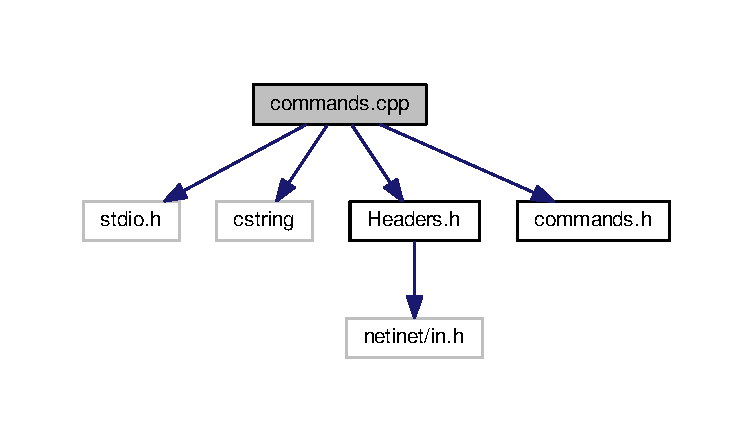
\includegraphics[width=350pt]{commands_8cpp__incl}
\end{center}
\end{figure}
\subsection*{Funzioni}
\begin{DoxyCompactItemize}
\item 
void \hyperlink{commands_8cpp_a666e101942c0878426bef303dd617c17}{parse\+Cmd} (char $\ast$cmd, char $\ast$buffer, int socket, sockaddr $\ast$client, socklen\+\_\+t len, \hyperlink{structconf}{conf} $\ast$cfgs, \hyperlink{structbackupThread}{backup\+Thread} $\ast$processi)\hypertarget{commands_8cpp_a666e101942c0878426bef303dd617c17}{}\label{commands_8cpp_a666e101942c0878426bef303dd617c17}

\begin{DoxyCompactList}\small\item\em Wrapper per i comandi, cmd\+\_\+parser. \end{DoxyCompactList}\end{DoxyCompactItemize}


\subsection{Descrizione dettagliata}
handler dei comandi 

\begin{DoxyVersion}{Versione}
1.\+0 
\end{DoxyVersion}
\begin{DoxyAuthor}{Autore}
Stefano 
\end{DoxyAuthor}
\begin{DoxyDate}{Data}
11-\/11-\/2017 
\end{DoxyDate}

\hypertarget{macros_8h}{}\section{Riferimenti per il file Compatibility/macros.h}
\label{macros_8h}\index{Compatibility/macros.\+h@{Compatibility/macros.\+h}}


Macro di compatibilità P\+O\+S\+IX linux-\/windows.  


Questo grafo mostra quali altri file includono direttamente o indirettamente questo file\+:\nopagebreak
\begin{figure}[H]
\begin{center}
\leavevmode
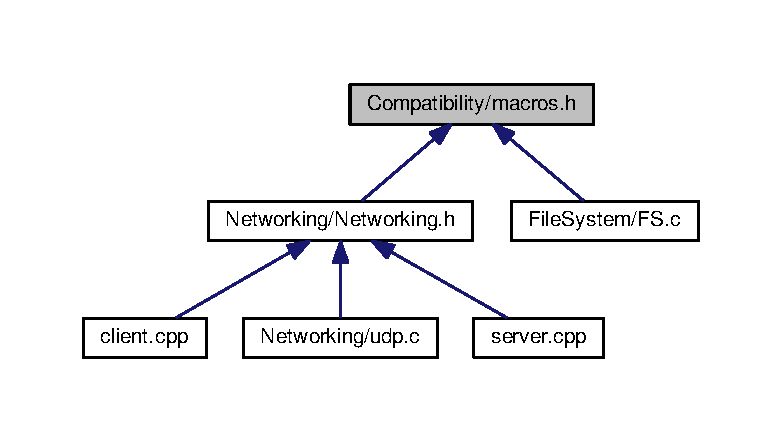
\includegraphics[width=350pt]{macros_8h__dep__incl}
\end{center}
\end{figure}


\subsection{Descrizione dettagliata}
Macro di compatibilità P\+O\+S\+IX linux-\/windows. 

\begin{DoxyVersion}{Versione}
1.\+0 
\end{DoxyVersion}
\begin{DoxyAuthor}{Autore}
Stefano 
\end{DoxyAuthor}
\begin{DoxyDate}{Data}
04-\/11-\/2017 
\end{DoxyDate}

\hypertarget{config_8c}{}\section{Riferimenti per il file config/config.c}
\label{config_8c}\index{config/config.\+c@{config/config.\+c}}


Operazioni sui file di configurazione.  


{\ttfamily \#include $<$stdio.\+h$>$}\\*
{\ttfamily \#include $<$malloc.\+h$>$}\\*
{\ttfamily \#include $<$memory.\+h$>$}\\*
{\ttfamily \#include \char`\"{}config.\+h\char`\"{}}\\*
Grafo delle dipendenze di inclusione per config.\+c\+:\nopagebreak
\begin{figure}[H]
\begin{center}
\leavevmode
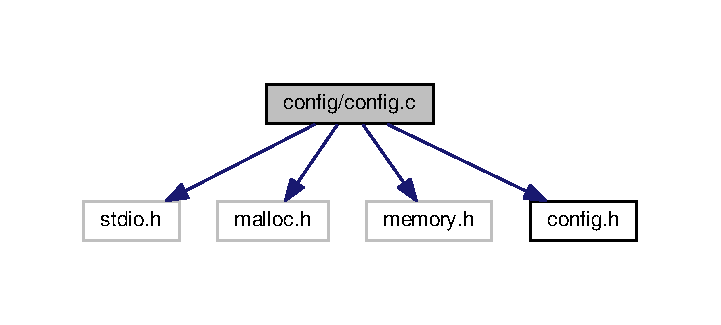
\includegraphics[width=346pt]{config_8c__incl}
\end{center}
\end{figure}
\subsection*{Funzioni}
\begin{DoxyCompactItemize}
\item 
char $\ast$$\ast$ \hyperlink{config_8c_a91b6fb28d1ce5cd7d4b72e112510b30c}{open\+Config\+File} (int $\ast$outlines, const char $\ast$filename, const char comment)
\begin{DoxyCompactList}\small\item\em Apre un file di configurazione per la lettura. Viene aperto e letto un file e salvato in memoria in un char $\ast$$\ast$, ignorando le linee di commento (carattere iniziale \textquotesingle{}\#\textquotesingle{}) e le linee vuote. \end{DoxyCompactList}\item 
char $\ast$ \hyperlink{config_8c_a8def4ff7352ba938cc05ae4b83550145}{get\+Property} (char $\ast$$\ast$file, int lines, const char $\ast$property, int lenght, int $\ast$is\+A\+List, int $\ast$list\+Len)
\begin{DoxyCompactList}\small\item\em Ottenimento di una proprietà dal file di configurazione. La funzione cerca linearmente la proprietà richiesta all\textquotesingle{}interno del file letto, e, nel caso la proprietà venga trovata, restituisce un puntatore alla stringa definita dalla proprietà nel file. Nel caso la proprietà richiesta sia una lista, viene restituito un puntatore a char con valore uguale alla lunghezza della lista, e l\textquotesingle{}intero is\+A\+List verrà settato a 1. \end{DoxyCompactList}\item 
void \hyperlink{config_8c_ab15e2eb276eee7f19da0fe8c84d50660}{close\+Config\+File} ()\hypertarget{config_8c_ab15e2eb276eee7f19da0fe8c84d50660}{}\label{config_8c_ab15e2eb276eee7f19da0fe8c84d50660}

\begin{DoxyCompactList}\small\item\em Chiusura del file di configurazione. \end{DoxyCompactList}\end{DoxyCompactItemize}
\subsection*{Variabili}
\begin{DoxyCompactItemize}
\item 
char $\ast$$\ast$ {\bfseries destination}\hypertarget{config_8c_a204855c67903c6d8340b9fa397588b0d}{}\label{config_8c_a204855c67903c6d8340b9fa397588b0d}

\end{DoxyCompactItemize}


\subsection{Descrizione dettagliata}
Operazioni sui file di configurazione. 

\begin{DoxyVersion}{Versione}
1.\+0 
\end{DoxyVersion}
\begin{DoxyAuthor}{Autore}
Stefano 
\end{DoxyAuthor}
\begin{DoxyDate}{Data}
07-\/11-\/2017 
\end{DoxyDate}


\subsection{Documentazione delle funzioni}
\index{config.\+c@{config.\+c}!get\+Property@{get\+Property}}
\index{get\+Property@{get\+Property}!config.\+c@{config.\+c}}
\subsubsection[{\texorpdfstring{get\+Property(char $\ast$$\ast$file, int lines, const char $\ast$property, int lenght, int $\ast$is\+A\+List, int $\ast$list\+Len)}{getProperty(char **file, int lines, const char *property, int lenght, int *isAList, int *listLen)}}]{\setlength{\rightskip}{0pt plus 5cm}char$\ast$ get\+Property (
\begin{DoxyParamCaption}
\item[{char $\ast$$\ast$}]{file, }
\item[{int}]{lines, }
\item[{const char $\ast$}]{property, }
\item[{int}]{lenght, }
\item[{int $\ast$}]{is\+A\+List, }
\item[{int $\ast$}]{list\+Len}
\end{DoxyParamCaption}
)}\hypertarget{config_8c_a8def4ff7352ba938cc05ae4b83550145}{}\label{config_8c_a8def4ff7352ba938cc05ae4b83550145}


Ottenimento di una proprietà dal file di configurazione. La funzione cerca linearmente la proprietà richiesta all\textquotesingle{}interno del file letto, e, nel caso la proprietà venga trovata, restituisce un puntatore alla stringa definita dalla proprietà nel file. Nel caso la proprietà richiesta sia una lista, viene restituito un puntatore a char con valore uguale alla lunghezza della lista, e l\textquotesingle{}intero is\+A\+List verrà settato a 1. 


\begin{DoxyParams}{Parametri}
{\em file\mbox{[}in\mbox{]}} & lista delle righe ritornata da open\+Config\+File \\
\hline
\end{DoxyParams}
\begin{DoxySeeAlso}{Si veda anche}
\hyperlink{config_8c_a91b6fb28d1ce5cd7d4b72e112510b30c}{open\+Config\+File} 
\end{DoxySeeAlso}

\begin{DoxyParams}{Parametri}
{\em lines\mbox{[}in\mbox{]}} & Lunghezza della lista \\
\hline
{\em property\mbox{[}in\mbox{]}} & Nome della proprietà da ricercare \\
\hline
{\em lenght\mbox{[}in\mbox{]}} & Lunghezza massima della lista di ritorno \\
\hline
{\em is\+A\+List\mbox{[}out\mbox{]}} & Se 1 il valore ritornato riguarda una lista, altrimenti 0 \\
\hline
{\em list\+Len\mbox{[}out\mbox{]}} & Se is\+A\+List == 1, indica la lunghezza della lista \\
\hline
\end{DoxyParams}
\begin{DoxyReturn}{Restituisce}
Un puntatore al valore della lista in caso la proprietà venga trovata, N\+U\+LL altrimenti. 
\end{DoxyReturn}
\index{config.\+c@{config.\+c}!open\+Config\+File@{open\+Config\+File}}
\index{open\+Config\+File@{open\+Config\+File}!config.\+c@{config.\+c}}
\subsubsection[{\texorpdfstring{open\+Config\+File(int $\ast$outlines, const char $\ast$filename, const char comment)}{openConfigFile(int *outlines, const char *filename, const char comment)}}]{\setlength{\rightskip}{0pt plus 5cm}char$\ast$$\ast$ open\+Config\+File (
\begin{DoxyParamCaption}
\item[{int $\ast$}]{outlines, }
\item[{const char $\ast$}]{filename, }
\item[{const char}]{comment}
\end{DoxyParamCaption}
)}\hypertarget{config_8c_a91b6fb28d1ce5cd7d4b72e112510b30c}{}\label{config_8c_a91b6fb28d1ce5cd7d4b72e112510b30c}


Apre un file di configurazione per la lettura. Viene aperto e letto un file e salvato in memoria in un char $\ast$$\ast$, ignorando le linee di commento (carattere iniziale \textquotesingle{}\#\textquotesingle{}) e le linee vuote. 


\begin{DoxyParams}{Parametri}
{\em outlines\mbox{[}out\mbox{]}} & Numero di linee lette \\
\hline
{\em filename\mbox{[}in\mbox{]}} & file di configurazione \\
\hline
{\em comment\mbox{[}in\mbox{]}} & Carattere di commento \\
\hline
\end{DoxyParams}
\begin{DoxyReturn}{Restituisce}
puntatore all\textquotesingle{}array di linee letto 
\end{DoxyReturn}

\hypertarget{extract_8cpp}{}\section{Riferimenti per il file extract.\+cpp}
\label{extract_8cpp}\index{extract.\+cpp@{extract.\+cpp}}


Utilità di estrazione di un file.  


{\ttfamily \#include \char`\"{}A\+E\+S/aes.\+h\char`\"{}}\\*
{\ttfamily \#include $<$stdio.\+h$>$}\\*
{\ttfamily \#include $<$inttypes.\+h$>$}\\*
{\ttfamily \#include $<$memory.\+h$>$}\\*
{\ttfamily \#include $<$cstdlib$>$}\\*
{\ttfamily \#include \char`\"{}Headers.\+h\char`\"{}}\\*
Grafo delle dipendenze di inclusione per extract.\+cpp\+:\nopagebreak
\begin{figure}[H]
\begin{center}
\leavevmode
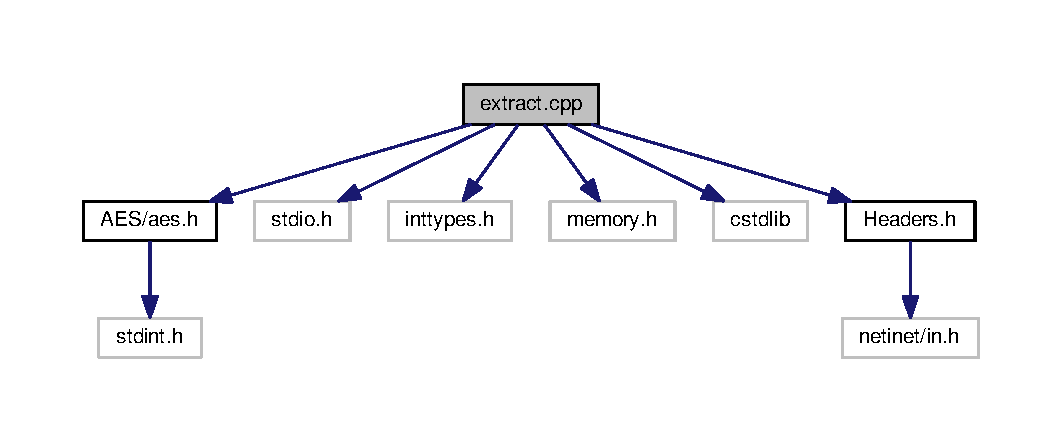
\includegraphics[width=350pt]{extract_8cpp__incl}
\end{center}
\end{figure}
\subsection*{Funzioni}
\begin{DoxyCompactItemize}
\item 
int {\bfseries main} (int argc, char $\ast$$\ast$argv)\hypertarget{extract_8cpp_a3c04138a5bfe5d72780bb7e82a18e627}{}\label{extract_8cpp_a3c04138a5bfe5d72780bb7e82a18e627}

\end{DoxyCompactItemize}
\subsection*{Variabili}
\begin{DoxyCompactItemize}
\item 
char {\bfseries key} \mbox{[}32\mbox{]}\hypertarget{extract_8cpp_aba8ec8b73c06b7c981b67e88184a1d08}{}\label{extract_8cpp_aba8ec8b73c06b7c981b67e88184a1d08}

\item 
char {\bfseries nome} \mbox{[}500\mbox{]}\hypertarget{extract_8cpp_a038a12ef5a4888ee35af7e15984d5983}{}\label{extract_8cpp_a038a12ef5a4888ee35af7e15984d5983}

\item 
uint8\+\_\+t $\ast$ {\bfseries data}\hypertarget{extract_8cpp_abe222f6d3581e7920dcad5306cc906a8}{}\label{extract_8cpp_abe222f6d3581e7920dcad5306cc906a8}

\end{DoxyCompactItemize}


\subsection{Descrizione dettagliata}
Utilità di estrazione di un file. 

\begin{DoxyVersion}{Versione}
1.\+0 
\end{DoxyVersion}
\begin{DoxyAuthor}{Autore}
Stefano 
\end{DoxyAuthor}
\begin{DoxyDate}{Data}
04-\/11-\/2017 
\end{DoxyDate}

\hypertarget{extract__all_8cpp}{}\section{Riferimenti per il file extract\+\_\+all.\+cpp}
\label{extract__all_8cpp}\index{extract\+\_\+all.\+cpp@{extract\+\_\+all.\+cpp}}


Utilità di estrazione dei file in una directory.  


{\ttfamily \#include \char`\"{}A\+E\+S/aes.\+h\char`\"{}}\\*
{\ttfamily \#include $<$stdio.\+h$>$}\\*
{\ttfamily \#include $<$inttypes.\+h$>$}\\*
{\ttfamily \#include $<$memory.\+h$>$}\\*
{\ttfamily \#include $<$cstdlib$>$}\\*
{\ttfamily \#include \char`\"{}File\+System/\+F\+S.\+h\char`\"{}}\\*
{\ttfamily \#include \char`\"{}Headers.\+h\char`\"{}}\\*
Grafo delle dipendenze di inclusione per extract\+\_\+all.\+cpp\+:\nopagebreak
\begin{figure}[H]
\begin{center}
\leavevmode
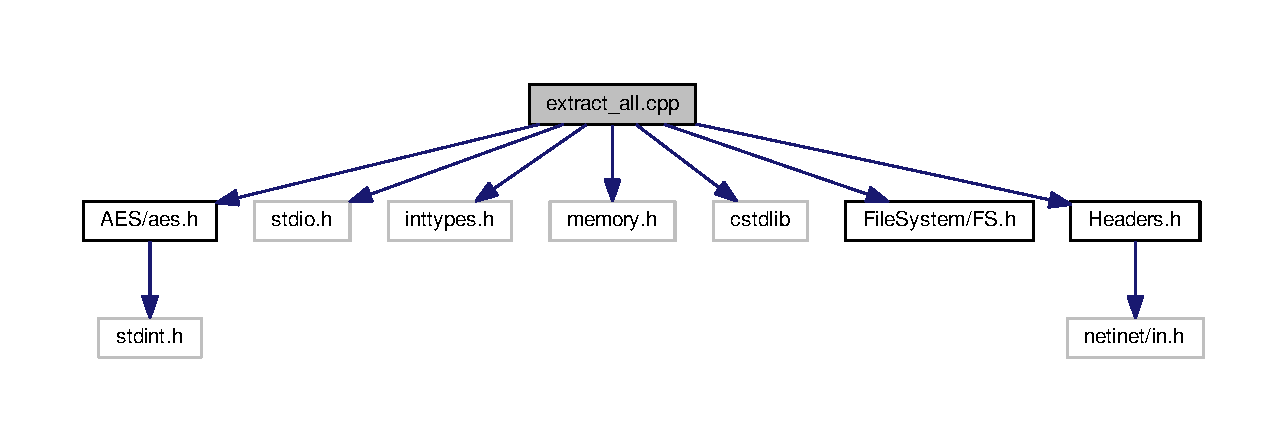
\includegraphics[width=350pt]{extract__all_8cpp__incl}
\end{center}
\end{figure}
\subsection*{Funzioni}
\begin{DoxyCompactItemize}
\item 
int {\bfseries extract} (int packet\+Size, char $\ast$key\+\_\+aes, char $\ast$file)\hypertarget{extract__all_8cpp_a7d4650f87c772c427c6bbca9e81005fd}{}\label{extract__all_8cpp_a7d4650f87c772c427c6bbca9e81005fd}

\item 
int {\bfseries main} (int argc, char $\ast$$\ast$argv)\hypertarget{extract__all_8cpp_a3c04138a5bfe5d72780bb7e82a18e627}{}\label{extract__all_8cpp_a3c04138a5bfe5d72780bb7e82a18e627}

\end{DoxyCompactItemize}
\subsection*{Variabili}
\begin{DoxyCompactItemize}
\item 
char {\bfseries key} \mbox{[}32\mbox{]}\hypertarget{extract__all_8cpp_aba8ec8b73c06b7c981b67e88184a1d08}{}\label{extract__all_8cpp_aba8ec8b73c06b7c981b67e88184a1d08}

\item 
char {\bfseries nome} \mbox{[}500\mbox{]}\hypertarget{extract__all_8cpp_a038a12ef5a4888ee35af7e15984d5983}{}\label{extract__all_8cpp_a038a12ef5a4888ee35af7e15984d5983}

\item 
uint8\+\_\+t $\ast$ {\bfseries data}\hypertarget{extract__all_8cpp_abe222f6d3581e7920dcad5306cc906a8}{}\label{extract__all_8cpp_abe222f6d3581e7920dcad5306cc906a8}

\end{DoxyCompactItemize}


\subsection{Descrizione dettagliata}
Utilità di estrazione dei file in una directory. 

\begin{DoxyVersion}{Versione}
1.\+0 
\end{DoxyVersion}
\begin{DoxyAuthor}{Autore}
Stefano 
\end{DoxyAuthor}
\begin{DoxyDate}{Data}
04-\/11-\/2017 
\end{DoxyDate}

\hypertarget{FS_8c}{}\section{Riferimenti per il file File\+System/\+FS.c}
\label{FS_8c}\index{File\+System/\+F\+S.\+c@{File\+System/\+F\+S.\+c}}


Operazioni sul File\+System.  


{\ttfamily \#include $<$malloc.\+h$>$}\\*
{\ttfamily \#include $<$string.\+h$>$}\\*
{\ttfamily \#include $<$dirent.\+h$>$}\\*
{\ttfamily \#include $<$stdio.\+h$>$}\\*
{\ttfamily \#include \char`\"{}../\+Compatibility/macros.\+h\char`\"{}}\\*
{\ttfamily \#include \char`\"{}F\+S.\+h\char`\"{}}\\*
Grafo delle dipendenze di inclusione per F\+S.\+c\+:\nopagebreak
\begin{figure}[H]
\begin{center}
\leavevmode
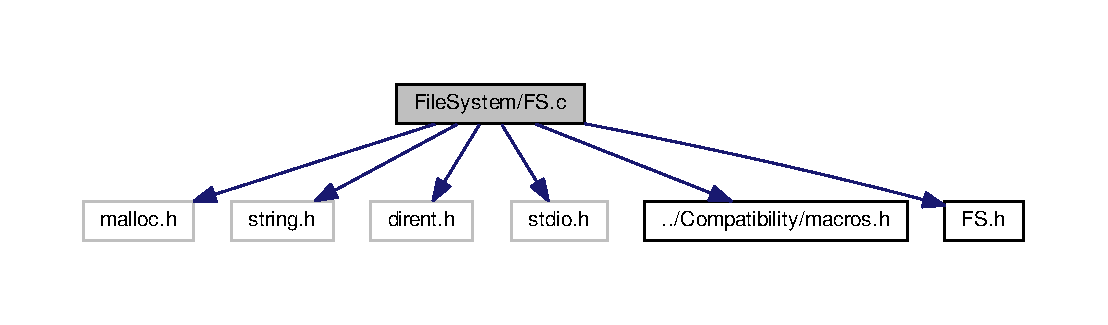
\includegraphics[width=350pt]{FS_8c__incl}
\end{center}
\end{figure}
\subsection*{Funzioni}
\begin{DoxyCompactItemize}
\item 
int \hyperlink{FS_8c_addcd589c251230573223a3a90130ce94}{is\+\_\+regular\+\_\+file} (const char $\ast$path)
\begin{DoxyCompactList}\small\item\em Determina se un file esiste o è una cartella. \end{DoxyCompactList}\item 
char $\ast$$\ast$ \hyperlink{FS_8c_a1b4278016bf88947be8f51137abeb270}{get\+Files} (char $\ast$mdir, int $\ast$len, int depth)
\begin{DoxyCompactList}\small\item\em Ottiene i file presenti in una cartella. \end{DoxyCompactList}\end{DoxyCompactItemize}


\subsection{Descrizione dettagliata}
Operazioni sul File\+System. 

\begin{DoxyVersion}{Versione}
1.\+0 
\end{DoxyVersion}
\begin{DoxyAuthor}{Autore}
Stefano 
\end{DoxyAuthor}
\begin{DoxyDate}{Data}
25-\/11-\/2017 
\end{DoxyDate}


\subsection{Documentazione delle funzioni}
\index{F\+S.\+c@{F\+S.\+c}!get\+Files@{get\+Files}}
\index{get\+Files@{get\+Files}!F\+S.\+c@{F\+S.\+c}}
\subsubsection[{\texorpdfstring{get\+Files(char $\ast$mdir, int $\ast$len, int depth)}{getFiles(char *mdir, int *len, int depth)}}]{\setlength{\rightskip}{0pt plus 5cm}char$\ast$$\ast$ get\+Files (
\begin{DoxyParamCaption}
\item[{char $\ast$}]{mdir, }
\item[{int $\ast$}]{len, }
\item[{int}]{depth}
\end{DoxyParamCaption}
)}\hypertarget{FS_8c_a1b4278016bf88947be8f51137abeb270}{}\label{FS_8c_a1b4278016bf88947be8f51137abeb270}


Ottiene i file presenti in una cartella. 

\begin{DoxyRefDesc}{Bug}
\item[\hyperlink{bug__bug000003}{Bug}]Ricorsione causa segfault per input errati \end{DoxyRefDesc}

\begin{DoxyParams}{Parametri}
{\em mdir\mbox{[}in\mbox{]}} & Directory \\
\hline
{\em len\mbox{[}out\mbox{]}} & Numero dei file trovati \\
\hline
{\em depth\mbox{[}in\mbox{]}} & Profondità di ricerca \\
\hline
\end{DoxyParams}
\begin{DoxyReturn}{Restituisce}
Puntatore alla lista dei file 
\end{DoxyReturn}
\index{F\+S.\+c@{F\+S.\+c}!is\+\_\+regular\+\_\+file@{is\+\_\+regular\+\_\+file}}
\index{is\+\_\+regular\+\_\+file@{is\+\_\+regular\+\_\+file}!F\+S.\+c@{F\+S.\+c}}
\subsubsection[{\texorpdfstring{is\+\_\+regular\+\_\+file(const char $\ast$path)}{is_regular_file(const char *path)}}]{\setlength{\rightskip}{0pt plus 5cm}int is\+\_\+regular\+\_\+file (
\begin{DoxyParamCaption}
\item[{const char $\ast$}]{path}
\end{DoxyParamCaption}
)}\hypertarget{FS_8c_addcd589c251230573223a3a90130ce94}{}\label{FS_8c_addcd589c251230573223a3a90130ce94}


Determina se un file esiste o è una cartella. 

\begin{DoxyRefDesc}{Bug}
\item[\hyperlink{bug__bug000002}{Bug}]File Inesistente o cartella inesistente causa segfault \end{DoxyRefDesc}

\begin{DoxyParams}{Parametri}
{\em path\mbox{[}in\mbox{]}} & File da verificare \\
\hline
\end{DoxyParams}
\begin{DoxyReturn}{Restituisce}

\end{DoxyReturn}

\hypertarget{md5_8c}{}\section{Riferimenti per il file M\+D5/md5.c}
\label{md5_8c}\index{M\+D5/md5.\+c@{M\+D5/md5.\+c}}


Hashing M\+D5.  


{\ttfamily \#include $<$stdio.\+h$>$}\\*
{\ttfamily \#include $<$stdlib.\+h$>$}\\*
{\ttfamily \#include $<$string.\+h$>$}\\*
{\ttfamily \#include $<$stdint.\+h$>$}\\*
{\ttfamily \#include \char`\"{}md5.\+h\char`\"{}}\\*
Grafo delle dipendenze di inclusione per md5.\+c\+:
% FIG 0
\subsection*{Definizioni}
\begin{DoxyCompactItemize}
\item 
\#define {\bfseries L\+E\+F\+T\+R\+O\+T\+A\+TE}(x,  c)~(((x) $<$$<$ (c)) $\vert$ ((x) $>$$>$ (32 -\/ (c))))\hypertarget{md5_8c_abceca7779c418db12903dbe2fa56bc21}{}\label{md5_8c_abceca7779c418db12903dbe2fa56bc21}

\end{DoxyCompactItemize}
\subsection*{Funzioni}
\begin{DoxyCompactItemize}
\item 
void \hyperlink{md5_8c_aa330d6bc857be530f7739e58af5cf0a8_aa330d6bc857be530f7739e58af5cf0a8}{md5} (uint8\+\_\+t $\ast$initial\+\_\+msg, size\+\_\+t initial\+\_\+len, char $\ast$ret)
\begin{DoxyCompactList}\small\item\em Computa l\textquotesingle{}M\+D5 di una stringa. \end{DoxyCompactList}\end{DoxyCompactItemize}
\subsection*{Variabili}
\begin{DoxyCompactItemize}
\item 
uint32\+\_\+t {\bfseries h0}\hypertarget{md5_8c_a3470604b2c9366033d0dc5855e9bd312}{}\label{md5_8c_a3470604b2c9366033d0dc5855e9bd312}

\item 
uint32\+\_\+t {\bfseries h1}\hypertarget{md5_8c_a1dabfc5f40ac6b7b9519070ac8b46d90}{}\label{md5_8c_a1dabfc5f40ac6b7b9519070ac8b46d90}

\item 
uint32\+\_\+t {\bfseries h2}\hypertarget{md5_8c_a24349a4077af3c0b286a2811032b7673}{}\label{md5_8c_a24349a4077af3c0b286a2811032b7673}

\item 
uint32\+\_\+t {\bfseries h3}\hypertarget{md5_8c_ad3b6541d7f6d4357ab1feebef30d4d62}{}\label{md5_8c_ad3b6541d7f6d4357ab1feebef30d4d62}

\end{DoxyCompactItemize}


\subsection{Descrizione dettagliata}
Hashing M\+D5. 

\begin{DoxyVersion}{Versione}
1.\+0 
\end{DoxyVersion}
\begin{DoxyAuthor}{Autore}
Stefano 
\end{DoxyAuthor}
\begin{DoxyDate}{Data}
23-\/11-\/2017 
\end{DoxyDate}


\subsection{Documentazione delle funzioni}
\index{md5.\+c@{md5.\+c}!md5@{md5}}
\index{md5@{md5}!md5.\+c@{md5.\+c}}
\subsubsection[{\texorpdfstring{md5(uint8\+\_\+t $\ast$initial\+\_\+msg, size\+\_\+t initial\+\_\+len, char $\ast$ret)}{md5(uint8_t *initial_msg, size_t initial_len, char *ret)}}]{\setlength{\rightskip}{0pt plus 5cm}void md5 (
\begin{DoxyParamCaption}
\item[{uint8\+\_\+t $\ast$}]{initial\+\_\+msg, }
\item[{size\+\_\+t}]{initial\+\_\+len, }
\item[{char $\ast$}]{ret}
\end{DoxyParamCaption}
)}\hypertarget{md5_8c_aa330d6bc857be530f7739e58af5cf0a8_aa330d6bc857be530f7739e58af5cf0a8}{}\label{md5_8c_aa330d6bc857be530f7739e58af5cf0a8_aa330d6bc857be530f7739e58af5cf0a8}


Computa l\textquotesingle{}M\+D5 di una stringa. 


\begin{DoxyParams}{Parametri}
{\em initial\+\_\+msg\mbox{[}in\mbox{]}} & Messaggio iniziale \\
\hline
{\em initial\+\_\+len\mbox{[}in\mbox{]}} & Lunghezza del messaggio \\
\hline
{\em ret\mbox{[}out\mbox{]}} & Hash (da preallocare) \\
\hline
\end{DoxyParams}

\hypertarget{udp_8c}{}\section{Riferimenti per il file Networking/udp.c}
\label{udp_8c}\index{Networking/udp.\+c@{Networking/udp.\+c}}


Funzioni di rete U\+DP.  


{\ttfamily \#include $<$stdio.\+h$>$}\\*
{\ttfamily \#include $<$sys/time.\+h$>$}\\*
{\ttfamily \#include \char`\"{}Networking.\+h\char`\"{}}\\*
Grafo delle dipendenze di inclusione per udp.\+c\+:
% FIG 0
\subsection*{Funzioni}
\begin{DoxyCompactItemize}
\item 
\hyperlink{structconnection__t}{connection\+\_\+t} \hyperlink{udp_8c_adbe079c402747c64e8a7ccdce80a9397_adbe079c402747c64e8a7ccdce80a9397}{new\+U\+D\+P\+Socket\+\_\+client} (const int portno, const char $\ast$host\+Name, const int timeout)
\begin{DoxyCompactList}\small\item\em Connette la macchina ad un server U\+DP. \end{DoxyCompactList}\item 
int \hyperlink{udp_8c_a1ed10c1ef4a1d2eb3b282332e028c51f_a1ed10c1ef4a1d2eb3b282332e028c51f}{new\+U\+D\+P\+Socket\+\_\+server} (const int portno)
\begin{DoxyCompactList}\small\item\em Crea un server U\+DP. \end{DoxyCompactList}\end{DoxyCompactItemize}


\subsection{Descrizione dettagliata}
Funzioni di rete U\+DP. 

\begin{DoxyVersion}{Versione}
1.\+0 
\end{DoxyVersion}
\begin{DoxyAuthor}{Autore}
Stefano 
\end{DoxyAuthor}
\begin{DoxyDate}{Data}
28-\/11-\/2017 
\end{DoxyDate}


\subsection{Documentazione delle funzioni}
\index{udp.\+c@{udp.\+c}!new\+U\+D\+P\+Socket\+\_\+client@{new\+U\+D\+P\+Socket\+\_\+client}}
\index{new\+U\+D\+P\+Socket\+\_\+client@{new\+U\+D\+P\+Socket\+\_\+client}!udp.\+c@{udp.\+c}}
\subsubsection[{\texorpdfstring{new\+U\+D\+P\+Socket\+\_\+client(const int portno, const char $\ast$host\+Name, const int timeout)}{newUDPSocket_client(const int portno, const char *hostName, const int timeout)}}]{\setlength{\rightskip}{0pt plus 5cm}{\bf connection\+\_\+t} new\+U\+D\+P\+Socket\+\_\+client (
\begin{DoxyParamCaption}
\item[{const int}]{portno, }
\item[{const char $\ast$}]{host\+Name, }
\item[{const int}]{timeout}
\end{DoxyParamCaption}
)}\hypertarget{udp_8c_adbe079c402747c64e8a7ccdce80a9397_adbe079c402747c64e8a7ccdce80a9397}{}\label{udp_8c_adbe079c402747c64e8a7ccdce80a9397_adbe079c402747c64e8a7ccdce80a9397}


Connette la macchina ad un server U\+DP. 


\begin{DoxyParams}{Parametri}
{\em portno\mbox{[}in\mbox{]}} & numero della porta di connessione \\
\hline
{\em host\+Name\mbox{[}in\mbox{]}} & Nome dell\textquotesingle{}host o I\+Pv4 \\
\hline
{\em timeout\mbox{[}in\mbox{]}} & Secondi di timeout prima dell\textquotesingle{}aborto della connessione \\
\hline
\end{DoxyParams}
\begin{DoxyReturn}{Restituisce}
parametri di connessione 
\end{DoxyReturn}
\index{udp.\+c@{udp.\+c}!new\+U\+D\+P\+Socket\+\_\+server@{new\+U\+D\+P\+Socket\+\_\+server}}
\index{new\+U\+D\+P\+Socket\+\_\+server@{new\+U\+D\+P\+Socket\+\_\+server}!udp.\+c@{udp.\+c}}
\subsubsection[{\texorpdfstring{new\+U\+D\+P\+Socket\+\_\+server(const int portno)}{newUDPSocket_server(const int portno)}}]{\setlength{\rightskip}{0pt plus 5cm}int new\+U\+D\+P\+Socket\+\_\+server (
\begin{DoxyParamCaption}
\item[{const int}]{portno}
\end{DoxyParamCaption}
)}\hypertarget{udp_8c_a1ed10c1ef4a1d2eb3b282332e028c51f_a1ed10c1ef4a1d2eb3b282332e028c51f}{}\label{udp_8c_a1ed10c1ef4a1d2eb3b282332e028c51f_a1ed10c1ef4a1d2eb3b282332e028c51f}


Crea un server U\+DP. 


\begin{DoxyParams}{Parametri}
{\em portno\mbox{[}in\mbox{]}} & Porta dove stanziare il server \\
\hline
\end{DoxyParams}
\begin{DoxyReturn}{Restituisce}
Intero descrittore del socket 
\end{DoxyReturn}

\hypertarget{packets_8c}{}\section{Riferimenti per il file packets.\+c}
\label{packets_8c}\index{packets.\+c@{packets.\+c}}


Metodi di compilazione strutture.  


{\ttfamily \#include \char`\"{}Headers.\+h\char`\"{}}\\*
Grafo delle dipendenze di inclusione per packets.\+c\+:\nopagebreak
\begin{figure}[H]
\begin{center}
\leavevmode
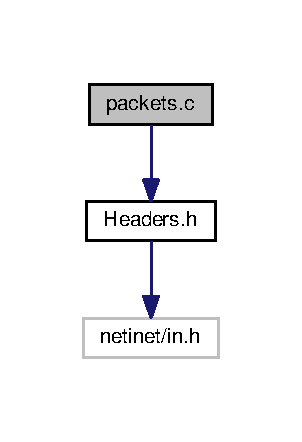
\includegraphics[width=145pt]{packets_8c__incl}
\end{center}
\end{figure}
\subsection*{Funzioni}
\begin{DoxyCompactItemize}
\item 
void {\bfseries make} (char $\ast$dest, const char $\ast$in)\hypertarget{packets_8c_a498a9049c2d27fa1395b0ec07073ede9}{}\label{packets_8c_a498a9049c2d27fa1395b0ec07073ede9}

\item 
\hyperlink{structmainpacket}{identify\+\_\+h} {\bfseries build\+Identify} ()\hypertarget{packets_8c_a22e8e02cb46d1196dab62a8feffefefa}{}\label{packets_8c_a22e8e02cb46d1196dab62a8feffefefa}

\item 
\hyperlink{structidentify__answ__h}{identify\+\_\+answ\+\_\+h} {\bfseries build\+Identify\+Answ} ()\hypertarget{packets_8c_aba0d9d89fecaefca156f72dcb90fb03b}{}\label{packets_8c_aba0d9d89fecaefca156f72dcb90fb03b}

\item 
\hyperlink{structmainpacket}{ask\+Pkey\+\_\+h} {\bfseries build\+Pkey\+Packet} ()\hypertarget{packets_8c_a6e3db20cdb55eaf675f2486d6256dffc}{}\label{packets_8c_a6e3db20cdb55eaf675f2486d6256dffc}

\item 
\hyperlink{structmainpacket}{new\+Bak\+\_\+h} {\bfseries build\+Bak\+Packet} ()\hypertarget{packets_8c_a41230729dfee19bf9c640df7c6cb288e}{}\label{packets_8c_a41230729dfee19bf9c640df7c6cb288e}

\end{DoxyCompactItemize}
\subsection*{Variabili}
\begin{DoxyCompactItemize}
\item 
const char {\bfseries id\+\_\+h} \mbox{[}$\,$\mbox{]} = \char`\"{}id\char`\"{}\hypertarget{packets_8c_a865e430fe73497618b4734c4ed2e334d}{}\label{packets_8c_a865e430fe73497618b4734c4ed2e334d}

\item 
const char {\bfseries pk\+\_\+h} \mbox{[}$\,$\mbox{]} = \char`\"{}pk\char`\"{}\hypertarget{packets_8c_a2d29498679b2b41bd06b803b41c2a94f}{}\label{packets_8c_a2d29498679b2b41bd06b803b41c2a94f}

\item 
const char {\bfseries answ\+\_\+h} \mbox{[}$\,$\mbox{]} = \char`\"{}as\char`\"{}\hypertarget{packets_8c_a5a31a944a12501ce2756c1afa124d800}{}\label{packets_8c_a5a31a944a12501ce2756c1afa124d800}

\item 
const char {\bfseries new\+\_\+h} \mbox{[}$\,$\mbox{]} = \char`\"{}ba\char`\"{}\hypertarget{packets_8c_a3d8067693ccb6446fd3125a70b5ec75d}{}\label{packets_8c_a3d8067693ccb6446fd3125a70b5ec75d}

\end{DoxyCompactItemize}


\subsection{Descrizione dettagliata}
Metodi di compilazione strutture. 

\begin{DoxyVersion}{Versione}
1.\+0 
\end{DoxyVersion}
\begin{DoxyAuthor}{Autore}
Stefano 
\end{DoxyAuthor}
\begin{DoxyDate}{Data}
31-\/10-\/2017 
\end{DoxyDate}

\hypertarget{server_8cpp}{}\section{Riferimenti per il file server.\+cpp}
\label{server_8cpp}\index{server.\+cpp@{server.\+cpp}}


Server.  


{\ttfamily \#include $<$cstdlib$>$}\\*
{\ttfamily \#include $<$signal.\+h$>$}\\*
{\ttfamily \#include $<$inttypes.\+h$>$}\\*
{\ttfamily \#include $<$sys/mman.\+h$>$}\\*
{\ttfamily \#include $<$stdio.\+h$>$}\\*
{\ttfamily \#include $<$time.\+h$>$}\\*
{\ttfamily \#include $<$fcntl.\+h$>$}\\*
{\ttfamily \#include \char`\"{}Networking/\+Networking.\+h\char`\"{}}\\*
{\ttfamily \#include \char`\"{}Headers.\+h\char`\"{}}\\*
{\ttfamily \#include \char`\"{}config/config.\+h\char`\"{}}\\*
{\ttfamily \#include \char`\"{}commands.\+h\char`\"{}}\\*
{\ttfamily \#include \char`\"{}Terminal/terminal.\+h\char`\"{}}\\*
Grafo delle dipendenze di inclusione per server.\+cpp\+:\nopagebreak
\begin{figure}[H]
\begin{center}
\leavevmode
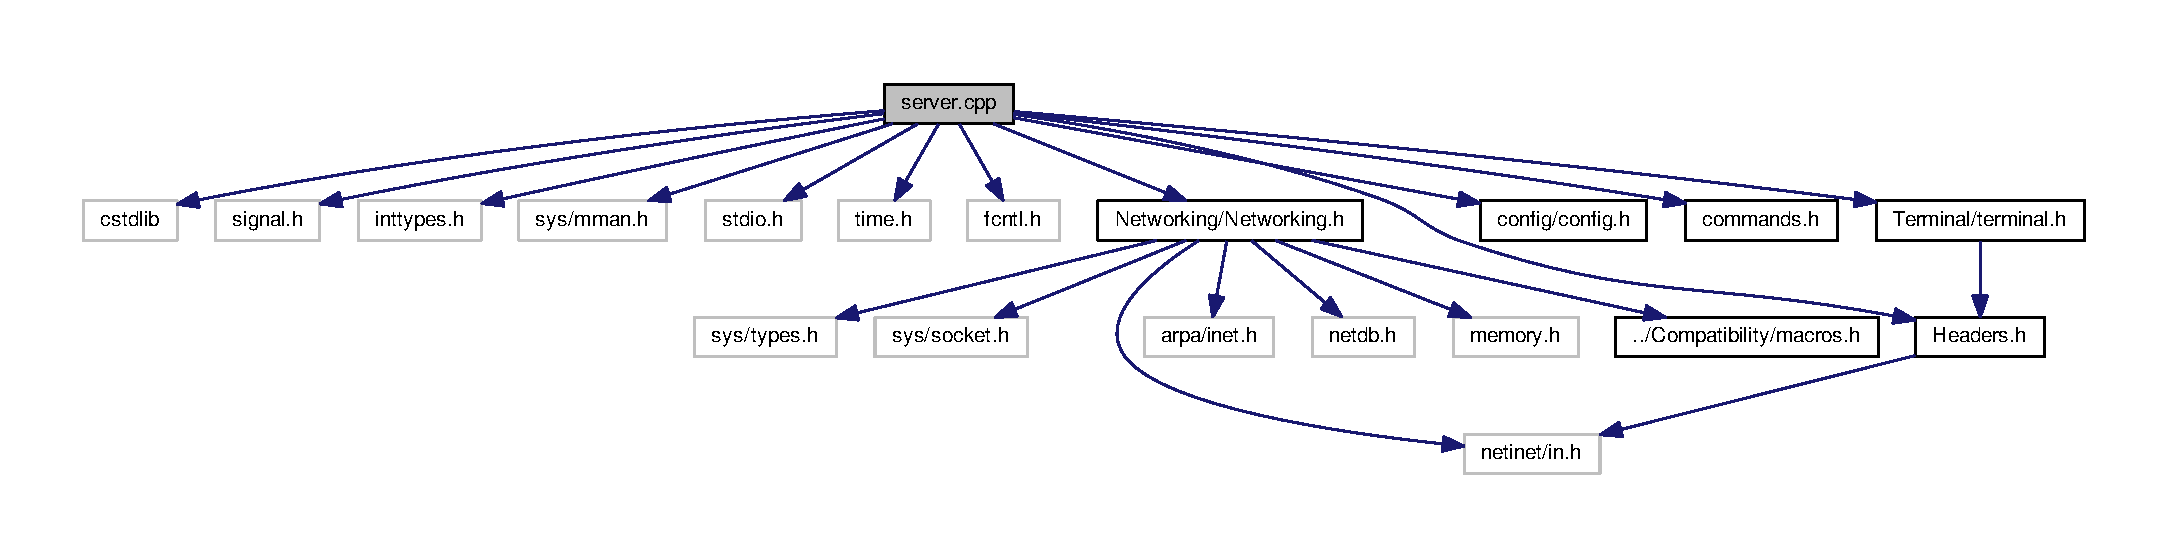
\includegraphics[width=350pt]{server_8cpp__incl}
\end{center}
\end{figure}
\subsection*{Definizioni}
\begin{DoxyCompactItemize}
\item 
\#define {\bfseries B\+Z\+F\+I\+LE}~F\+I\+LE\hypertarget{server_8cpp_a285a10d6860f8c385c5d7ea07e24a35d}{}\label{server_8cpp_a285a10d6860f8c385c5d7ea07e24a35d}

\end{DoxyCompactItemize}
\subsection*{Funzioni}
\begin{DoxyCompactItemize}
\item 
void \hyperlink{server_8cpp_a3b33e6f48f5d988f336e915c5346eb95}{int\+Handler} (int dummy)
\begin{DoxyCompactList}\small\item\em Handler per S\+I\+G\+H\+UP e S\+I\+G\+I\+NT Chiude le connessioni aperte e esce dal programma. \end{DoxyCompactList}\item 
int \hyperlink{server_8cpp_aed66b47e9b9d15f8c82424c1e3ab73cb}{load\+Cfg} ()
\begin{DoxyCompactList}\small\item\em Caricamento della configurazione da file. \end{DoxyCompactList}\item 
void \hyperlink{server_8cpp_a960a002a3603a6ca57072fa35ca14895}{send\+Pkey} (int socket, sockaddr to, socklen\+\_\+t len)
\begin{DoxyCompactList}\small\item\em Invia la chiave pubblica ad un client richiedente Invia due interi conteneti le lunghezze dei parametri spediti conseguentemente. \end{DoxyCompactList}\item 
void \hyperlink{server_8cpp_a5eabf61df48c377358c330d24affd4e8}{send\+Identification} (int socket, sockaddr to, socklen\+\_\+t len, \hyperlink{structmainpacket}{identify\+\_\+h} data)
\begin{DoxyCompactList}\small\item\em Risposta alla richiesta di identità \end{DoxyCompactList}\item 
int {\bfseries get\+Slot} (\hyperlink{structbackupThread}{backup\+Thread} $\ast$threads, int port\+\_\+ext)\hypertarget{server_8cpp_ab6accd513572d70f9f654567e16b0572}{}\label{server_8cpp_ab6accd513572d70f9f654567e16b0572}

\item 
void \hyperlink{server_8cpp_a0cd98657d687771b6bd634f8a65c14a2}{new\+Backup} (int socket, sockaddr to, socklen\+\_\+t len, \hyperlink{structmainpacket}{new\+Bak\+\_\+h} data)
\begin{DoxyCompactList}\small\item\em Avvia un processo di backup In caso di presenza della libreria B\+Z2 i file ricevuti verranno compressi se di dimensione inferiore a quella prestabilita. \end{DoxyCompactList}\item 
int \hyperlink{server_8cpp_a49bba8146fb528ffd39048b13361d3c3}{check\+\_\+host\+\_\+validity} (sockaddr\+\_\+in $\ast$client)
\begin{DoxyCompactList}\small\item\em Controlla che un host sia abilitato al dialogo con il server. La lista di host viene inserita nel file di configurazione. \end{DoxyCompactList}\item 
int {\bfseries main} (void)\hypertarget{server_8cpp_a840291bc02cba5474a4cb46a9b9566fe}{}\label{server_8cpp_a840291bc02cba5474a4cb46a9b9566fe}

\end{DoxyCompactItemize}
\subsection*{Variabili}
\begin{DoxyCompactItemize}
\item 
int {\bfseries server}\hypertarget{server_8cpp_ad41e465b11575618bf82f1d45efced5a}{}\label{server_8cpp_ad41e465b11575618bf82f1d45efced5a}

\item 
\hyperlink{structnetwork}{network} $\ast$ {\bfseries allowed\+Networks}\hypertarget{server_8cpp_a699884cb2dcd746c95a20b9fe066c4fd}{}\label{server_8cpp_a699884cb2dcd746c95a20b9fe066c4fd}

\item 
\hyperlink{unionipAddr}{ip\+Addr} $\ast$ {\bfseries allowed\+Hosts}\hypertarget{server_8cpp_ab8e6e12d81fbec012e792ca9a48ae3c2}{}\label{server_8cpp_ab8e6e12d81fbec012e792ca9a48ae3c2}

\item 
\hyperlink{unionipAddr}{ip\+Addr} $\ast$ {\bfseries managers}\hypertarget{server_8cpp_aecf5a55bcbbde8282ad30274d19024d1}{}\label{server_8cpp_aecf5a55bcbbde8282ad30274d19024d1}

\item 
\hyperlink{structconf}{conf} {\bfseries configs}\hypertarget{server_8cpp_ad6a1160de63172ff2b4a019048631a95}{}\label{server_8cpp_ad6a1160de63172ff2b4a019048631a95}

\item 
\hyperlink{structsshconf}{sshconf} {\bfseries sshconfigs}\hypertarget{server_8cpp_acf06d876d0472d02099cd61c7406a15d}{}\label{server_8cpp_acf06d876d0472d02099cd61c7406a15d}

\item 
int {\bfseries usessh} = 0\hypertarget{server_8cpp_a1cd99b9016dd1013134ce98853496447}{}\label{server_8cpp_a1cd99b9016dd1013134ce98853496447}

\item 
char $\ast$ {\bfseries rsacfg}\hypertarget{server_8cpp_a6dd5ce1d6191fd796288b6679e051b1c}{}\label{server_8cpp_a6dd5ce1d6191fd796288b6679e051b1c}

\item 
\hyperlink{structbackupThread}{backup\+Thread} $\ast$ {\bfseries processi}\hypertarget{server_8cpp_aefec74c965ba143be9258e692d8a287d}{}\label{server_8cpp_aefec74c965ba143be9258e692d8a287d}

\item 
char $\ast$$\ast$ {\bfseries file}\hypertarget{server_8cpp_ab8055e05865bc04373bc4e75fedf2d19}{}\label{server_8cpp_ab8055e05865bc04373bc4e75fedf2d19}

\end{DoxyCompactItemize}


\subsection{Descrizione dettagliata}
Server. 

\begin{DoxyVersion}{Versione}
1.\+0 
\end{DoxyVersion}
\begin{DoxyAuthor}{Autore}
Stefano 
\end{DoxyAuthor}
\begin{DoxyDate}{Data}
28-\/10-\/2017 
\end{DoxyDate}


\subsection{Documentazione delle funzioni}
\index{server.\+cpp@{server.\+cpp}!check\+\_\+host\+\_\+validity@{check\+\_\+host\+\_\+validity}}
\index{check\+\_\+host\+\_\+validity@{check\+\_\+host\+\_\+validity}!server.\+cpp@{server.\+cpp}}
\subsubsection[{\texorpdfstring{check\+\_\+host\+\_\+validity(sockaddr\+\_\+in $\ast$client)}{check_host_validity(sockaddr_in *client)}}]{\setlength{\rightskip}{0pt plus 5cm}int check\+\_\+host\+\_\+validity (
\begin{DoxyParamCaption}
\item[{sockaddr\+\_\+in $\ast$}]{client}
\end{DoxyParamCaption}
)}\hypertarget{server_8cpp_a49bba8146fb528ffd39048b13361d3c3}{}\label{server_8cpp_a49bba8146fb528ffd39048b13361d3c3}


Controlla che un host sia abilitato al dialogo con il server. La lista di host viene inserita nel file di configurazione. 


\begin{DoxyParams}{Parametri}
{\em client\mbox{[}in\mbox{]}} & descrittore del client connesso \\
\hline
\end{DoxyParams}
\index{server.\+cpp@{server.\+cpp}!int\+Handler@{int\+Handler}}
\index{int\+Handler@{int\+Handler}!server.\+cpp@{server.\+cpp}}
\subsubsection[{\texorpdfstring{int\+Handler(int dummy)}{intHandler(int dummy)}}]{\setlength{\rightskip}{0pt plus 5cm}void int\+Handler (
\begin{DoxyParamCaption}
\item[{int}]{dummy}
\end{DoxyParamCaption}
)}\hypertarget{server_8cpp_a3b33e6f48f5d988f336e915c5346eb95}{}\label{server_8cpp_a3b33e6f48f5d988f336e915c5346eb95}


Handler per S\+I\+G\+H\+UP e S\+I\+G\+I\+NT Chiude le connessioni aperte e esce dal programma. 


\begin{DoxyParams}{Parametri}
{\em dummy} & \\
\hline
\end{DoxyParams}
\index{server.\+cpp@{server.\+cpp}!load\+Cfg@{load\+Cfg}}
\index{load\+Cfg@{load\+Cfg}!server.\+cpp@{server.\+cpp}}
\subsubsection[{\texorpdfstring{load\+Cfg()}{loadCfg()}}]{\setlength{\rightskip}{0pt plus 5cm}int load\+Cfg (
\begin{DoxyParamCaption}
{}
\end{DoxyParamCaption}
)}\hypertarget{server_8cpp_aed66b47e9b9d15f8c82424c1e3ab73cb}{}\label{server_8cpp_aed66b47e9b9d15f8c82424c1e3ab73cb}


Caricamento della configurazione da file. 

\begin{DoxyReturn}{Restituisce}
0 in caso di riuscita, -\/1 altrimenti 
\end{DoxyReturn}
\begin{DoxyRefDesc}{Bug}
\item[\hyperlink{bug__bug000004}{Bug}]In caso una proprietà non sia presente segfault \end{DoxyRefDesc}
\index{server.\+cpp@{server.\+cpp}!new\+Backup@{new\+Backup}}
\index{new\+Backup@{new\+Backup}!server.\+cpp@{server.\+cpp}}
\subsubsection[{\texorpdfstring{new\+Backup(int socket, sockaddr to, socklen\+\_\+t len, new\+Bak\+\_\+h data)}{newBackup(int socket, sockaddr to, socklen_t len, newBak_h data)}}]{\setlength{\rightskip}{0pt plus 5cm}void new\+Backup (
\begin{DoxyParamCaption}
\item[{int}]{socket, }
\item[{sockaddr}]{to, }
\item[{socklen\+\_\+t}]{len, }
\item[{{\bf new\+Bak\+\_\+h}}]{data}
\end{DoxyParamCaption}
)}\hypertarget{server_8cpp_a0cd98657d687771b6bd634f8a65c14a2}{}\label{server_8cpp_a0cd98657d687771b6bd634f8a65c14a2}


Avvia un processo di backup In caso di presenza della libreria B\+Z2 i file ricevuti verranno compressi se di dimensione inferiore a quella prestabilita. 


\begin{DoxyParams}{Parametri}
{\em socket\mbox{[}in\mbox{]}} & descrittore del socket del server \\
\hline
{\em to\mbox{[}in\mbox{]}} & Descrittore dell\textquotesingle{}host cliente \\
\hline
{\em len\mbox{[}in\mbox{]}} & lunghezza di to \\
\hline
{\em data\mbox{[}in\mbox{]}} & Informazioni relative al backup da effettuare \\
\hline
\end{DoxyParams}
\index{server.\+cpp@{server.\+cpp}!send\+Identification@{send\+Identification}}
\index{send\+Identification@{send\+Identification}!server.\+cpp@{server.\+cpp}}
\subsubsection[{\texorpdfstring{send\+Identification(int socket, sockaddr to, socklen\+\_\+t len, identify\+\_\+h data)}{sendIdentification(int socket, sockaddr to, socklen_t len, identify_h data)}}]{\setlength{\rightskip}{0pt plus 5cm}void send\+Identification (
\begin{DoxyParamCaption}
\item[{int}]{socket, }
\item[{sockaddr}]{to, }
\item[{socklen\+\_\+t}]{len, }
\item[{{\bf identify\+\_\+h}}]{data}
\end{DoxyParamCaption}
)}\hypertarget{server_8cpp_a5eabf61df48c377358c330d24affd4e8}{}\label{server_8cpp_a5eabf61df48c377358c330d24affd4e8}


Risposta alla richiesta di identità 


\begin{DoxyParams}{Parametri}
{\em socket\mbox{[}in\mbox{]}} & descrittore del socket del server \\
\hline
{\em to\mbox{[}in\mbox{]}} & Descrittore dell\textquotesingle{}host cliente \\
\hline
{\em len\mbox{[}in\mbox{]}} & lunghezza di to \\
\hline
{\em data\mbox{[}in\mbox{]}} & Stringa da firmare \\
\hline
\end{DoxyParams}
\index{server.\+cpp@{server.\+cpp}!send\+Pkey@{send\+Pkey}}
\index{send\+Pkey@{send\+Pkey}!server.\+cpp@{server.\+cpp}}
\subsubsection[{\texorpdfstring{send\+Pkey(int socket, sockaddr to, socklen\+\_\+t len)}{sendPkey(int socket, sockaddr to, socklen_t len)}}]{\setlength{\rightskip}{0pt plus 5cm}void send\+Pkey (
\begin{DoxyParamCaption}
\item[{int}]{socket, }
\item[{sockaddr}]{to, }
\item[{socklen\+\_\+t}]{len}
\end{DoxyParamCaption}
)}\hypertarget{server_8cpp_a960a002a3603a6ca57072fa35ca14895}{}\label{server_8cpp_a960a002a3603a6ca57072fa35ca14895}


Invia la chiave pubblica ad un client richiedente Invia due interi conteneti le lunghezze dei parametri spediti conseguentemente. 


\begin{DoxyParams}{Parametri}
{\em socket\mbox{[}in\mbox{]}} & descrittore del socket del server \\
\hline
{\em to\mbox{[}in\mbox{]}} & Descrittore dell\textquotesingle{}host cliente \\
\hline
{\em len\mbox{[}in\mbox{]}} & lunghezza di to \\
\hline
\end{DoxyParams}

\hypertarget{terminal_8c}{}\section{Riferimenti per il file Terminal/terminal.c}
\label{terminal_8c}\index{Terminal/terminal.\+c@{Terminal/terminal.\+c}}


Utilità di firma di un eseguibile.  


{\ttfamily \#include $<$stdlib.\+h$>$}\\*
{\ttfamily \#include $<$stdio.\+h$>$}\\*
{\ttfamily \#include $<$string.\+h$>$}\\*
{\ttfamily \#include $<$signal.\+h$>$}\\*
{\ttfamily \#include $<$dlfcn.\+h$>$}\\*
{\ttfamily \#include \char`\"{}terminal.\+h\char`\"{}}\\*
{\ttfamily \#include \char`\"{}../\+M\+D5/md5.\+h\char`\"{}}\\*
Grafo delle dipendenze di inclusione per terminal.\+c\+:\nopagebreak
\begin{figure}[H]
\begin{center}
\leavevmode
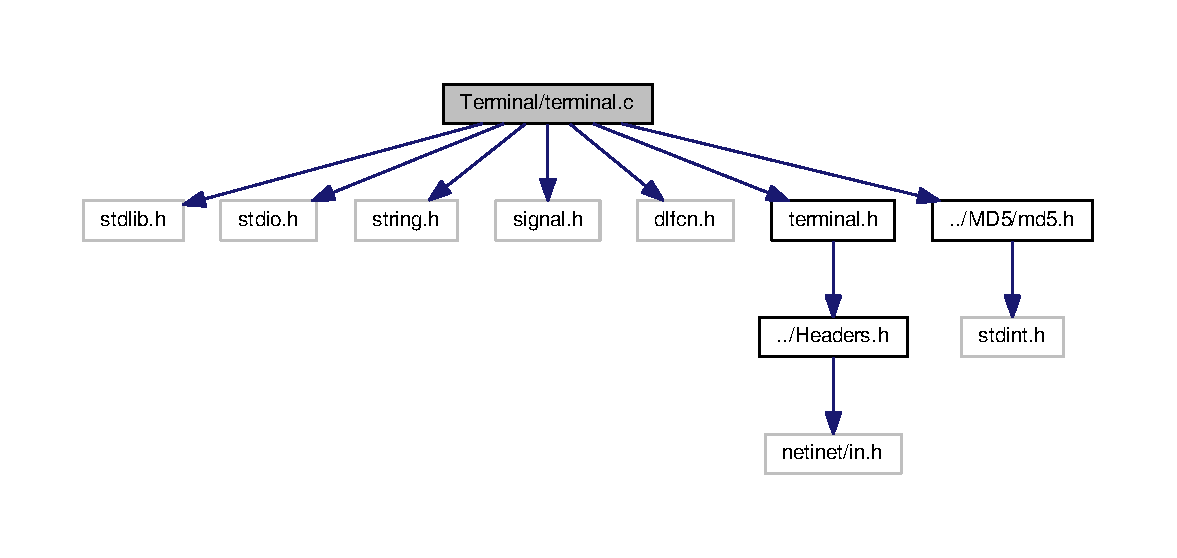
\includegraphics[width=350pt]{terminal_8c__incl}
\end{center}
\end{figure}
\subsection*{Funzioni}
\begin{DoxyCompactItemize}
\item 
void \hyperlink{terminal_8c_a2cce86fa8d3ac0c27fea942a6bf8a3c7}{parse\+Command} (char $\ast$command, size\+\_\+t len, \hyperlink{structbackupThread}{backup\+Thread} $\ast$baks, \hyperlink{structconf}{conf} $\ast$cfgs, int($\ast$print\+To\+Stream)(const char $\ast$format,...))
\begin{DoxyCompactList}\small\item\em Identifica il comando Viene trovato il comando, se esiste viene controllata la firma digitale con i parametri pubblici in memoria e viene quindi eseguito il codice. \end{DoxyCompactList}\item 
void \hyperlink{terminal_8c_acd70420842ce412f1204b9e2761958ee}{init\+\_\+terminal} (pid\+\_\+t serverpid, \hyperlink{structbackupThread}{backup\+Thread} $\ast$baks, \hyperlink{structconf}{conf} $\ast$cfgs)
\begin{DoxyCompactList}\small\item\em Inizializzazione del termiale. \end{DoxyCompactList}\end{DoxyCompactItemize}
\subsection*{Variabili}
\begin{DoxyCompactItemize}
\item 
char {\bfseries bf} \mbox{[}2048\mbox{]}\hypertarget{terminal_8c_a0f68fa947f6a42edf7d2b75660fa8e12}{}\label{terminal_8c_a0f68fa947f6a42edf7d2b75660fa8e12}

\item 
char $\ast$ {\bfseries bufffer}\hypertarget{terminal_8c_abe9213b9472e131a492125901e6d9c96}{}\label{terminal_8c_abe9213b9472e131a492125901e6d9c96}

\item 
char $\ast$ {\bfseries elf}\hypertarget{terminal_8c_aa356e0c7cced7496fa77653f2176a98d}{}\label{terminal_8c_aa356e0c7cced7496fa77653f2176a98d}

\item 
char {\bfseries md} \mbox{[}16\mbox{]}\hypertarget{terminal_8c_a61bafde6f010fb965e7089aef189e7b9}{}\label{terminal_8c_a61bafde6f010fb965e7089aef189e7b9}

\item 
char {\bfseries fooo} \mbox{[}33\mbox{]}\hypertarget{terminal_8c_a9f6c41c2b3ee7c6d5a8850189f99b748}{}\label{terminal_8c_a9f6c41c2b3ee7c6d5a8850189f99b748}

\end{DoxyCompactItemize}


\subsection{Descrizione dettagliata}
Utilità di firma di un eseguibile. 

Gestione terminale.

\begin{DoxyVersion}{Versione}
1.\+0 
\end{DoxyVersion}
\begin{DoxyAuthor}{Autore}
Stefano 
\end{DoxyAuthor}
\begin{DoxyDate}{Data}
23-\/11-\/2017
\end{DoxyDate}
\begin{DoxyVersion}{Versione}
1.\+0 
\end{DoxyVersion}
\begin{DoxyAuthor}{Autore}
Stefano 
\end{DoxyAuthor}
\begin{DoxyDate}{Data}
18-\/11-\/2017 
\end{DoxyDate}


\subsection{Documentazione delle funzioni}
\index{terminal.\+c@{terminal.\+c}!init\+\_\+terminal@{init\+\_\+terminal}}
\index{init\+\_\+terminal@{init\+\_\+terminal}!terminal.\+c@{terminal.\+c}}
\subsubsection[{\texorpdfstring{init\+\_\+terminal(pid\+\_\+t serverpid, backup\+Thread $\ast$baks, conf $\ast$cfgs)}{init_terminal(pid_t serverpid, backupThread *baks, conf *cfgs)}}]{\setlength{\rightskip}{0pt plus 5cm}void init\+\_\+terminal (
\begin{DoxyParamCaption}
\item[{pid\+\_\+t}]{serverpid, }
\item[{{\bf backup\+Thread} $\ast$}]{baks, }
\item[{{\bf conf} $\ast$}]{cfgs}
\end{DoxyParamCaption}
)}\hypertarget{terminal_8c_acd70420842ce412f1204b9e2761958ee}{}\label{terminal_8c_acd70420842ce412f1204b9e2761958ee}


Inizializzazione del termiale. 


\begin{DoxyParams}{Parametri}
{\em serverpid\mbox{[}in\mbox{]}} & P\+ID del server \\
\hline
{\em baks\mbox{[}in\mbox{]}} & Referenza al vettore di processi di backup \\
\hline
\end{DoxyParams}
\begin{DoxySeeAlso}{Si veda anche}
\hyperlink{server_8cpp}{server.\+cpp} 
\end{DoxySeeAlso}

\begin{DoxyParams}{Parametri}
{\em cfgs\mbox{[}in\mbox{]}} & Referenza alla cconfigurazione del server \\
\hline
\end{DoxyParams}
\index{terminal.\+c@{terminal.\+c}!parse\+Command@{parse\+Command}}
\index{parse\+Command@{parse\+Command}!terminal.\+c@{terminal.\+c}}
\subsubsection[{\texorpdfstring{parse\+Command(char $\ast$command, size\+\_\+t len, backup\+Thread $\ast$baks, conf $\ast$cfgs, int($\ast$print\+To\+Stream)(const char $\ast$format,...))}{parseCommand(char *command, size_t len, backupThread *baks, conf *cfgs, int(*printToStream)(const char *format,...))}}]{\setlength{\rightskip}{0pt plus 5cm}void parse\+Command (
\begin{DoxyParamCaption}
\item[{char $\ast$}]{command, }
\item[{size\+\_\+t}]{len, }
\item[{{\bf backup\+Thread} $\ast$}]{baks, }
\item[{{\bf conf} $\ast$}]{cfgs, }
\item[{int($\ast$)(const char $\ast$format,...)}]{print\+To\+Stream}
\end{DoxyParamCaption}
)}\hypertarget{terminal_8c_a2cce86fa8d3ac0c27fea942a6bf8a3c7}{}\label{terminal_8c_a2cce86fa8d3ac0c27fea942a6bf8a3c7}


Identifica il comando Viene trovato il comando, se esiste viene controllata la firma digitale con i parametri pubblici in memoria e viene quindi eseguito il codice. 


\begin{DoxyParams}{Parametri}
{\em command\mbox{[}in\mbox{]}} & Stringa del comando con gli argomenti \\
\hline
{\em len\mbox{[}in\mbox{]}} & Lunghezza della stringa del comando \\
\hline
{\em baks\mbox{[}in\mbox{]}} & Referenza al vettore di processi di backup \\
\hline
\end{DoxyParams}
\begin{DoxySeeAlso}{Si veda anche}
\hyperlink{server_8cpp}{server.\+cpp} 
\end{DoxySeeAlso}

\begin{DoxyParams}{Parametri}
{\em cfgs\mbox{[}in\mbox{]}} & Referenza alla cconfigurazione del server \\
\hline
{\em print\+To\+Stream\mbox{[}in\mbox{]}} & Funzione di stampa \\
\hline
\end{DoxyParams}

%--- End generated contents ---

% Index
\backmatter
\newpage
\phantomsection
\clearemptydoublepage
\addcontentsline{toc}{chapter}{Indice}
\printindex

\end{document}
